\documentclass[10pt,twoside,a4paper]{memoir}
\usepackage[ascii]{}
\usepackage[T1]{fontenc}
\usepackage{longtable}
\usepackage[utf8]{inputenc}
\usepackage{lmodern}
\usepackage{lettrine}
\usepackage{geometry}
\usepackage{amsmath,amssymb,amsfonts,textcomp}
\usepackage{color}
\usepackage[dvipsnames]{xcolor}
\usepackage{colortbl}
\usepackage{graphicx}
\usepackage{fancyhdr}
\usepackage{fancybox}
\usepackage{fancyvrb}
\usepackage[open=true]{bookmark}
\usepackage{caption}
\usepackage{listings}
\usepackage{array,multirow,multicol}
\usepackage{lastpage}
\usepackage{cellspace}
\usepackage{enumitem}
\usepackage{babel}
\usepackage{float}
\usepackage{chngcntr}
\usepackage{wrapfig}
\usepackage{tcolorbox}
\usepackage{tikz}
\usetikzlibrary{arrows}
\usetikzlibrary{decorations.pathreplacing}
\usepackage{tikzpagenodes}
\usepackage{pdflscape}
% espacement table des matieres et des figures entre numero et titre
\usepackage{tocloft}
\renewcommand{\cftpartnumwidth}{3em}
\cftsetindents{figure}{0em}{4em}
\cftsetindents{table}{0em}{4em}
%
% Pour supprimer les encadres rouges des liens et definir leur fonte en bleu
\usepackage{makeidx}
\usepackage{hyperref}
\hypersetup{linkcolor=blue,colorlinks=true,bookmarks=true,bookmarksopen=true,bookmarksnumbered=true}

\setlength{\arrayrulewidth}{1.5pt}%
\setlength\hoffset{0cm}
\setlength\voffset{0cm}
\setlength\oddsidemargin{0cm}
\setlength\evensidemargin{0cm}
\setlength\topmargin{0cm}
\setlength\headheight{0.45cm}
\setlength\headsep{0.8cm} %0.6
\setlength\marginparsep{0cm}
\setlength\marginparwidth{0cm}
\setlength\footskip{0.6cm} %1.4
\setlength{\textheight}{670pt} 
\setlength\textwidth{16.4cm}
\setlength{\cellspacebottomlimit}{5pt}
\setlength{\cellspacetoplimit}{5pt}
\setlength{\parindent}{0pt}
\setcounter{tocdepth}{2}
\setsecnumdepth{section}
% espacement corps de texte
\baselineskip=14pt
%
% redefinition de la numerotation des figures et des tableaux
\renewcommand{\thefigure}{\Roman{part}.\arabic{chapter}.\arabic{figure}}
\renewcommand{\thetable}{\Roman{part}.\arabic{chapter}.\arabic{table}}
%
\makeatletter
%% Because html converters don't know tabularnewline
\floatstyle{ruled}\providecommand{\tabularnewline}{\\}
%% nouvelle commande algorithm pour des zones de code
\floatstyle{ruled}
\newfloat{algorithm}{tbp}{loa}[chapter]
\providecommand{\algorithmname}{Algorithm}
\floatname{algorithm}{\protect\algorithmname}
%
\makeatother
%
\fancypagestyle{part}{%
\fancyhead[L]{}
\fancyhead[R]{\textit{\rightmark}}
\lfoot{\textit{TrioCFD Validation, v\codeVersion}}
\cfoot{}
\rfoot{\thepage}
\renewcommand{\headrulewidth}{0.5pt}
\renewcommand{\footrulewidth}{0.3pt}}
%
\fancypagestyle{chapter}{%
\fancyhead[L]{\textit{\rightmark}}
\fancyhead[R]{}
\lfoot{\textit{TrioCFD Validation, v\codeVersion}}
\cfoot{}
\rfoot{\thepage}
\renewcommand{\headrulewidth}{0.5pt}
\renewcommand{\footrulewidth}{0.3pt}}
%
\pagestyle{fancy}
\renewcommand{\chaptermark}[1]{\markboth{#1}{#1}}
\renewcommand{\sectionmark}[1]{\markright{#1}}
\renewcommand{\headrulewidth}{0.5pt}
\renewcommand{\footrulewidth}{0.3pt}
\lhead{\leftmark}
\chead{}
\rhead{\rightmark}
\lfoot{\textit{TrioCFD Validation, v\codeVersion}}
\cfoot{}
\rfoot{\thepage}
%
% definition du style des parties
\usepackage{indentfirst}
\renewcommand{\beforepartskip}{\null\vskip 5pt plus 1.8fil \newpage}
\renewcommand{\afterpartskip}{\vskip 0pt plus 0.7fil }
\renewcommand*{\partnumfont}{\normalfont\HUGE\sffamily}
\renewcommand*{\parttitlefont}{\normalfont\Huge\sffamily}
\renewcommand{\part}[1]{%
  \phantomsection
  \refstepcounter{part}%
  \addcontentsline{toc}{part}%
    {\protect\partnumberline{\thepart}#1}
  \pagestyle{part}
  \beforepartskip
  \printpartnum. \space \printparttitle{#1}
  \afterpartskip
  }
% definition du style des chapitres
%
\renewcommand{\clearforchapter}{\null\vskip 1pt}

\makechapterstyle{customchapstyle}{%
  \pagestyle{chapter}
  \clearforchapter
  \renewcommand*{\chapnumfont}{\normalfont\HUGE\sffamily}
  \renewcommand*{\chaptitlefont}{\normalfont\huge\sffamily}
  \settowidth{\chapindent}{\chapnumfont 111}
  \renewcommand*{\chapterheadstart}{\begingroup
    \vspace*{\beforechapskip}%
    \begin{adjustwidth}{}{}%
    \hrulefill
    \smash{\rule{0.4pt}{15mm}}
    \end{adjustwidth}\endgroup}
  \renewcommand*{\printchaptername}{}
  \renewcommand*{\chapternamenum}{}
  \renewcommand*{\printchapternum}{%
    \begin{adjustwidth}{}{}
    \hfill
    \raisebox{10mm}[0pt][0pt]{\chapnumfont \Roman{part}.\thechapter}%
                              \hspace*{1em}
    \end{adjustwidth}\vspace*{-3.0\onelineskip}}
  \renewcommand*{\printchaptertitle}[1]{%
    \vskip\onelineskip
    \raggedleft {\chaptitlefont ##1}\par\nobreak}}
%
\counterwithin*{chapter}{part}
%

% Variables definition
% - TrioCFD version
\newcommand\codeVersion{1.9.3}
% - Number of validation report
\newcommand\nbValidationReports{198}

\makeindex
%%%%%%%%%%%%%%%%%%%%%%%%%%%%%%%%%%%%%%%%%%%%%%%%%%%%%%%%%%%%%%%%%%%%%%%%%%%%%%%%%%%%%%
% debut du document
%%%%%%%%%%%%%%%%%%%%%%%%%%%%%%%%%%%%%%%%%%%%%%%%%%%%%%%%%%%%%%%%%%%%%%%%%%%%%%%%%%%%%%
\begin{document}
%
% 1ere page
\thispagestyle{empty}
%\cfoot{}
%\renewcommand{\headrulewidth}{0pt}
%\renewcommand{\footrulewidth}{0pt}
\begin{multicols}{2}

\includegraphics[scale=0.75]{tools/cea-logo.png}
\begin{flushright}\Ovalbox{\begin{minipage}{8cm} \begin{center} \vspace{0.4cm}\Large{DES/ISAS/DM2S/STMF/LMSF}\vspace{0.4cm}\end{center}\end{minipage}}\end{flushright}
\begin{flushright}\Ovalbox{\begin{minipage}{4cm} \begin{center} \vspace{0.4cm}\Large{\thepage/\pageref{LastPage}}\vspace{0.4cm}\end{center}\end{minipage}}\end{flushright}
\end{multicols}
\cornersize{.2}
\Ovalbox{\begin{minipage}{16.2cm}
\begin{center}
\vspace{1.5cm}
\parbox[t]{12cm}{\hspace{1.3cm}\huge{\textbf{USER DOCUMENTATION :}}
\vspace{0.4cm}\newline 
\hspace{5cm}\LARGE{\textbf{Validation Report for TrioCFD v\codeVersion}}}
\end{center}
\vspace{0.3cm}
\begin{center}
\includegraphics[scale=0.65]{tools/Trio-CFD.png} \end{center}
\vspace{0.3cm}
\begin{center}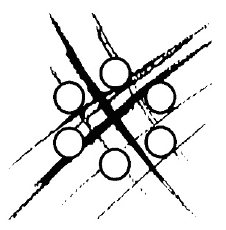
\includegraphics[scale=0.65]{tools/DM2S.png} \end{center}
\vspace{0.4cm}
\setlength{\tabcolsep}{0.5cm}

\begin{tabular}{ Sc|Sc|Sc|Sc }
\hline
Code Version & Date & Code manager & Authors \\
\hline
v\codeVersion  & \today &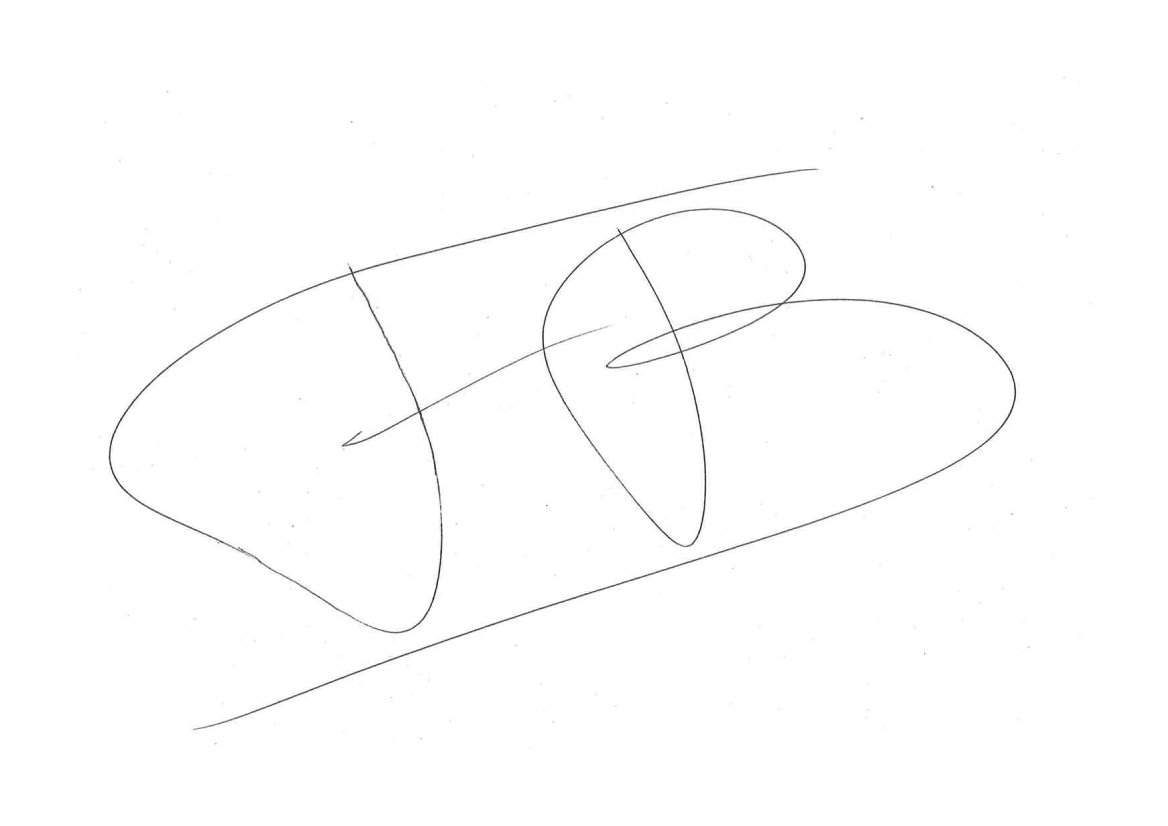
\includegraphics[scale=0.05]{../pictures/signTrioCFDManager.png} & TrioCFD Team \\
               &        & F. BUFFA                                      & \\
\hline
\multicolumn{2}{Sc|}{ } & \multicolumn{2}{Sl}{\textit{Input file : } validation\_report\_TrioCFD.tex } \\
\multicolumn{2}{c|}{\textbf{DES/ISAS/DM2S} } & \multicolumn{2}{l}{\textit{Software : } TrioCFD } \\
\multicolumn{2}{c|}{\textbf{CEA SACLAY} } & \multicolumn{2}{c}{ } \\
\cline{3-4}
\multicolumn{2}{c|}{\textbf{91191 GIF-SUR-YVETTE CEDEX} } & \multicolumn{2}{c}{ } \\
\multicolumn{2}{Sc|}{ } & \multicolumn{2}{Sc}{\large{\textbf{DES/ISAS/DM2S/STMF/LMSF/UD}} } \\
\multicolumn{2}{c|}{ } & \multicolumn{2}{c}{ } \\
\end{tabular}
\end{minipage}}
\newpage
%
%
% Style chapitres
\chapterstyle{customchapstyle}
%
\tableofcontents
\clearpage
%
\listoffigures
%
\vspace{6cm}
\listoftables
%
%%%%%%%%%%%%%%%%%%%%%%%%%%%%%%%%%%%%%%%%%%%%%%%%%%%%%%%%%%%%%%%%%%%%%%%%%%%%%%%%%%%%%%
\part{Introduction}
\markright{INTRODUCTION}
\normalsize \normalfont
\vspace{4.5cm}
\rhead{INTRODUCTION}
\lhead{}

\lettrine[lines=2,slope=0pt,nindent=4pt]{\textbf{L}}{a} Gestion de Configuration Logicielle (GCL) est une discipline de management de projet qui permet de d\'efinir,
d'identifier, de g\'erer et de contr\^oler les outils de configuration tout au long du cycle de d\'eveloppement d'un
logiciel. Cette gestion de configuration logicielle est r\'egie par la norme internationale ISO 10007:2017 \cite{normISO}. Le respect des normes internationales en terme de gestion de configuration est indispensable pour tout code, d'autant plus lorsque celui-ci est utilisé dans le cadre de la sûreté nucléaire comme l'est TrioCFD. Elle a pour objectif de r\'epondre \`a la question : " Quelqu'un a obtenu un r\'esultat. Comment le reproduire ? " Le plus souvent, il ne s'agit pas de reproduire \`a l'identique, mais de reproduire avec des modifications incr\'ementales. La question est donc de comparer des r\'esultats et d'analyser leurs diff\'erences.\smallskip\newline
La gestion de configuration du logiciel se concentre sur les aspects informatiques du logiciel et du syst\`eme qui le concerne. Ainsi, la GCL s'appuie sur la gestion de version pour pouvoir identifier avec fiabilité la version du logiciel utilis\'e, mais prend \'egalement en compte l'environnement mat\'eriel (machines h\^otes, \'equipements en interface) et syst\`eme (syst\`eme d'exploitation, type de r\'eseau,...) dans lequel celui-ci fonctionne.\newline
Elle s'attache \'egalement \`a tracer le suivi des \'evolutions (correctifs, \'evolutions) en regard des adaptations du produit. A ce titre, un outil de type \textit{syst\`eme de suivi de probl\`emes (issue tracking system)} est fortement recommand\'e dans le processus de gestion. Les adaptations qui en d\'ecoulent se font en veillant en maintenir \`a jour la matrice de conformit\'e qui garantit l'assurance fonctionnelle du produit.\smallskip\newline
En r\'esum\'e, g\'erer la configuration d'un logiciel consiste \`a g\'erer :
\begin{itemize}
	\item les diff\'erentes versions de ses composants (code, outils, donn\'ees de v\'erification/validation,...)
	\item sa documentation
	\item les anomalies et les r\'eponses apport\'ees \`a leur r\'esolution
	\item les demandes de modification ou d'\'evolution
	\item les environnements : espaces de d\'eveloppement, de v\'erification, de validation, de production
\end{itemize}

Cela consiste \'egalement \`a d\'efinir les r\`egles de passage d'un environnement \`a l'autre. Cette m\'ethodologie apporte au g\'enie logiciel les moyens de r\'ealiser un produit logiciel avec une qualit\'e et une ma\^itrise du processus de d\'eveloppement \'elev\'ees.\smallskip\newline
La Gestion de Configuration Logicielle permet de nombreux b\'en\'efices :
\begin{itemize}
	\item fournit une approche disciplinée et documentée pour d\'efinir, organiser et maintenir les \'el\'ements applicatifs,
	\item garantit l'int\'egrit\'e des applications,
	\item assure que les versions pr\'ec\'edentes de tout livrable contr\^ol\'e par configuration peuvent \^etre restaur\'ees et recr\'e\'ees,
	\item assure que tous les changements ne sont r\'ealis\'es que lorsque cela est requis et seulement par les personnes autoris\'ees.
\end{itemize}

Le Plan de Gestion de Configuration (PGC) permet, quant \`a lui, de fournir \`a l'\'equipe de d\'eveloppement et de validation du logiciel une m\'ethodologie de travail et une description de l'utilisation des  outils afin de r\'epondre aux exigences de fiabilit\'e qui leur sont demand\'ees. LE PGC est utilis\'e comme base pour r\'ealiser l'ensemble des activit\'es sur le code (maintenance, d\'eveloppement, correction, gestion de version, livraison,...).\smallskip\newline

L'objectif de ce Plan de Gestion de Configuration (PGC) de TrioCFD est donc de d\'efinir, pour les diff\'erents acteurs intervenants sur TrioCFD, les m\'ethodologies pour r\'esoudre les diff\'erentes actions qu'ils ont en charge, les outils \`a leur disposition ainsi que la documentation n\'ecessaire \`a la bonne utilisation du code.\smallskip\newline
Pour ce faire, nous commencerons par nous int\'eresser aux diff\'erents termes et acteurs de TrioCFD, puis aux outils de gestion. Les outils techniques sp\'ecifiques seront ensuite d\'ecrits ainsi que la m\'ethodologie de v\'erification et de validation. Nous finirons par la description de la conduite \'a tenir pour chacune des actions possibles sur le produit et les outils de communication autour de TrioCFD. Mais d\'ebutons, tout d'abord, par un petit historique de TrioCFD et une pr\'esentation g\'en\'erale de la structure du code.

\chapter{Un peu d'histoire}
\rhead{INTRODUCTION}
\lhead{Un peu d'histoire}

\lettrine[lines=2,slope=0pt,nindent=4pt]{\textbf{L}}{e} d\'eveloppement de TRIO\_U a d\'ebut\'e en 1994 au CEA de Grenoble avec l'ambition d'unifier TRIO VF, d\'evelopp\'e \`a Grenoble, Trio EF, d\'evelopp\'e \`a Saclay, et Genepi.\smallskip\newline
L'id\'ee initiale \'etait de cr\'eer un seul code unifi\'e (d'o\`u le \_U de TRIO\_U) code dans un langage plus r\'ecent \`a savoir le C++ puisque TRIO VF et Genepi \'etaient en Esope, TRIO EF en FORTRAN. Une premi\`ere maquette avait \'et\'e réalisée en se basant
sur le principe de cr\'eer une classe C++ par maille. Or, cette m\'ethodologie nécessitait des ressources machine beaucoup trop cons\'equentes pour les calculs fins. Un nouveau maquettage a \'et\'e alors réalisé avec une classe C++ par probl\`eme (Conduction, Hydraulique,...), par \'equation (\textit{e.g.} EDP), par op\'erateur (gradient, divergence, laplacien,...), par variable physique ($rho$, $mu$,..),... C'est cette seconde structure qui a \'et\'e finalement retenue et qui est, aujourd'hui encore, appliqu\'ee dans TRUST et ses Baltiks.\smallskip\newline
En ce qui concerne l'unification des codes, celle-ci ne s'est finalement pas faite et TRIO\_U a donc d\'ebut\'e uniquement avec TRIO VF et été d\'evelopp\'e sur Grenoble jusqu'\`a la migration du service de Thermohydraulique de Grenoble vers Saclay dans les ann\'ees 2010. Genepi est rest\'e un code ind\'ependant. Quant \`a TRIO EF, son d\'eveloppement n'a pas \'et\'e poursuivi.\smallskip\newline
Au fil des ann\'ees, les mod\`eles, fonctionnalit\'es et outils du code ont \'et\'e enrichis progressivement. L'historique de ces principales am\'eliorations sont pr\'ecis\'ees dans la frise chronologique \ref{figure:Histo-triou}.\smallskip\newline
En 2015, TRIO\_U v1.7.1 a \'et\'e scind\'e en deux parties : TrioCFD et TRUST. 
Cette s\'eparation entre TRUST et TrioCFD a \'et\'e faite de mani\`ere à ce que le code TRUST contienne toute la partie \texttt{noyau logiciel (kernel)} \'a savoir les op\'erateurs, les solveurs, la discr\'etisation, les outils de maillage et de post-traitement, les sch\'emas en espace et en temps et le parall\'elisme. TRUST est ainsi capable de r\'esoudre de mani\`ere autonome des probl\`emes laminaires monophasiques incompressibles ou quasi-compressibles en 2D ou 3D. TrioCFD regroupe, quant \`a lui, la partie \texttt{mod\`eles physiques pouss\'es pour la CFD} comme la turbulence
(LES et RANS), le diphasique (Front-tracking et Interface diffuse), les interactions fluide-structure (m\'ethode ALE),... Ces mod\`eles physiques sont rang\'es dans des modules distincts appel\'es \texttt{Baltik} faisant de TrioCFD un code modulaire.\newpage
\footnotesize
%\scriptsize
\begin{tikzpicture}
	\draw (8,0) -- (8,18.52) ;
	\draw (0,0) -- (0,0.01) ;
	\draw (7.8,18.52) -- (8.2,18.52) ;
	\draw (7.8,18.52) node[left]{$1994$} ;
	\draw[blue,thick,dashed] (8.0,18.52) -- (8.7,18.52) ;
	\draw[red] (8.8,18.52) node[right]{D\'ebut du projet Trio\_U} ;
	\draw[magenta,thick,dashed] (6.3,18.52) -- (7.0,18.52) ;
	\draw (6.2,18.52) node[left]{\textcolor{magenta}{Version en Unix}} ;
	\draw[decorate ,decoration={brace,amplitude=10pt,raise=0.5cm}] (8.35,18.32) -- (8.35,16.2) node[midway,right=1cm]{Maquettage};
	\draw (7.8,18.10) -- (8.0,18.10) ;
	\draw (7.8,17.68) -- (8.2,17.68) ;
	\draw (7.8,17.68) node[left]{$1995$} ;
	\draw (7.8,17.26) -- (8.0,17.26) ;
	\draw (7.8,16.84) -- (8.2,16.84) ;
	\draw (7.8,16.84) node[left]{$1996$} ;
	\draw[magenta,thick,dashed] (6.3,16.84) -- (7.0,16.84) ;
	\draw (6.2,16.84) node[left]{\textcolor{magenta}{Passage en gestion de configuration sous SCCS}} ;
	\draw (7.8,16.42) -- (8.0,16.42) ;
	\draw (7.8,16.00) -- (8.2,16.00) ;
	\draw (7.8,16.00) node[left]{$1997$} ;
	\draw[blue,thick,dashed] (8.0,16.00) -- (8.7,16.00) ;
	\draw (8.8,16.00) node[right]{\textcolor{blue}{v1.0} Discr\'etisation VDF seulement} ;
	\draw[green,thick,dashed] (6.3,16.00) -- (7.0,16.00) ;
	\draw[green] (6.2,16.00) node[left]{Mise en place des TNR} ;
	\draw (7.8,15.58) -- (8.0,15.58) ;
	\draw (7.8,15.16) -- (8.2,15.16) ;
	\draw (7.8,15.16) node[left]{$1998$} ;
	\draw[magenta,thick,dashed] (8.0,15.16) -- (8.7,15.16) ;
	\draw[magenta] (8.8,15.16) node[right]{Changement de gestionnaire de configuration : ClearCase} ;
	\draw[magenta,thick,dashed] (6.4,15.16) -- (7.0,15.16) ;
	\draw[magenta,thick,dashed] (6.4,15.37) -- (6.4,14.85) ;
	\draw[magenta,thick,dashed] (6.4,15.37) -- (6.3,15.37) ;
	\draw[magenta,thick,dashed] (6.4,14.85) -- (6.3,14.85) ;
	\draw[magenta] (6.2,15.37) node[left]{$1^{\`ere}$ Version Linux} ;
	\draw[magenta] (6.2,14.95) node[left]{$1^{\`ere}$ Maquette de parall\'elisme pour les machines CRAY} ;
	\draw (7.8,14.74) -- (8.0,14.74) ;
	\draw[blue,thick,dashed] (8.0,14.74) -- (8.7,14.74) ;
	\draw (8.8,14.74) node[right]{\textcolor{blue}{v1.1} Ajout de la discr\'etisation VEF} ;
	\draw (7.8,14.32) -- (8.2,14.32) ;
	\draw (7.8,14.32) node[left]{$1999$} ;
	\draw[cyan,thick,dashed] (8.0,14.32) -- (8.7,14.32) ;
	\draw[cyan] (8.8,14.32) node[right]{Visualisation des r\'esultats avec meshDV} ;
	\draw[cyan,thick,dashed] (6.3,14.32) -- (7.0,14.32) ;
	\draw[cyan] (6.2,14.32) node[left]{Interface avec Ansys ICEM CFD} ;
	\draw[cyan] (6.2,14.01) node[left]{(g\'en\'eration automatique du maillage pour TrioCFD)} ;
	\draw (7.8,13.90) -- (8.0,13.90) ;
	\draw (7.8,13.48) -- (8.2,13.48) ;
	\draw (7.8,13.48) node[left]{$2000$} ;
	\draw (7.8,13.06) -- (8.0,13.06) ;
	\draw[blue,thick,dashed] (8.0,13.06) -- (8.7,13.06) ;
	\draw[magenta] (8.8,13.06) node[right]{\textcolor{blue}{v1.2} $1^{\`ere}$ Version parall\`ele officielle} ;
	\draw (7.8,12.64) -- (8.2,12.64) ;
	\draw (7.8,12.64) node[left]{$2001$} ;
	\draw (7.8,12.22) -- (8.0,12.22) ;
	\draw[blue,thick,dashed] (8.0,12.22) -- (8.7,12.22) ;
	\draw (8.8,12.22) node[right]{\textcolor{blue}{v1.3} \textbf{Module} Rayonnement : mod\`eles de radiation} ;
	\draw (7.8,11.80) -- (8.2,11.80) ;
	\draw (7.8,11.80) node[left]{$2002$} ;
	\draw (7.8,11.38) -- (8.0,11.38) ;
	\draw[blue,thick,dashed] (8.0,11.27) -- (8.7,11.27) ;
	\draw (8.8,11.27) node[right]{\textcolor{blue}{v1.4} \textbf{Module} Turbulence : Ajout de nouveaux } ;
	\draw (10.0,10.87) node[right]{mod\`eles de turbulence pour la LES} ;
	\draw (7.8,10.96) -- (8.2,10.96) ;
	\draw (7.8,10.96) node[left]{$2003$} ;
	\draw[black,thick,dashed] (6.3,10.96) -- (7.0,10.96) ;
	\draw (6.2,10.96) node[left]{$1^{\`ere}$ version utilisable du Quasi-Compressible} ;
	\draw (7.8,10.54) -- (8.0,10.54) ;
	\draw (7.8,10.12) -- (8.2,10.12) ;
	\draw (7.8,10.12) node[left]{$2004$} ;
	\draw[cyan,thick,dashed] (8.0,10.12) -- (8.7,10.12) ;
	\draw[cyan] (8.8,10.12) node[right]{Remplacement de meshDV par VisIT} ;
	\draw[cyan,thick,dashed] (6.4,10.12) -- (7.0,10.12) ;
	\draw[cyan,thick,dashed] (6.4,10.33) -- (6.4,09.91) ;
	\draw[cyan,thick,dashed] (6.4,10.33) -- (6.3,10.33) ;
	\draw[cyan,thick,dashed] (6.4,09.91) -- (6.3,09.91) ;
	\draw[cyan] (6.2,10.33) node[left]{Utilisation du format MED} ;
	\draw[cyan] (6.2,09.91) node[left]{Interfa\c cage avec SALOME pour le maillage} ;
	\draw (7.8,09.70) -- (8.0,09.70) ;
	\draw (7.8,09.28) -- (8.2,09.28) ;
	\draw (7.8,09.28) node[left]{$2005$} ;
	\draw (7.8,08.86) -- (8.0,08.86) ;
	\draw (7.8,08.44) -- (8.2,08.44) ;
	\draw (7.8,08.44) node[left]{$2006$} ;
	\draw[blue,thick,dashed] (8.0,08.30) -- (8.7,08.30) ;
	\draw (8.8,08.30) node[right]{\textcolor{blue}{v1.5} \textbf{Module} Front-Tracking discontinu en VDF et VEF} ;
	\draw (7.8,08.02) -- (8.0,08.02) ;
	\draw (7.8,07.60) -- (8.2,07.60) ;
	\draw (7.8,07.60) node[left]{$2007$} ;
	\draw[magenta,thick,dashed] (6.3,07.60) -- (7.0,07.60) ;
	\draw[magenta] (6.2,07.60) node[left]{Interface de couplage ICoCo} ;
	\draw (7.8,07.18) -- (8.0,07.18) ;
	\draw[magenta,thick,dashed] (8.0,07.18) -- (8.7,07.18) ;
	\draw[magenta] (8.8,07.18) node[right]{Introduction de la notion de \texttt{BALTIK}} ;
	\draw (7.8,06.76) -- (8.2,06.76) ;
	\draw (7.8,06.76) node[left]{$2008$} ;
	\draw[magenta,thick,dashed] (8.0,06.76) -- (8.7,06.76) ;
	\draw[magenta] (8.8,06.76) node[right]{Introduction du solveur de syst\`emes lin\'eaires : PetSC} ;
	\draw[green,thick,dashed] (6.3,06.76) -- (7.0,06.76) ;
	\draw[green] (6.2,06.76) node[left]{Mise en place des fiches de validation automatiques} ;
	\draw (7.8,06.34) -- (8.0,06.34) ;
	\draw[magenta,thick,dashed] (6.3,06.21) -- (8.0,06.21) ;
	\draw (6.2,06.21) node[left]{\textcolor{blue}{v1.6} \textcolor{magenta}{Refonte de la structure des donn\'ees}} ;
	\draw (7.8,05.92) -- (8.2,05.92) ;
	\draw (7.8,05.92) node[left]{$2009$} ;
	\draw (7.8,05.50) -- (8.0,05.50) ;
	\draw (7.8,05.08) -- (8.2,05.08) ;
	\draw (7.8,05.08) node[left]{$2010$} ;
	\draw[magenta,thick,dashed] (8.0,05.08) -- (8.7,05.08) ;
	\draw[magenta] (8.8,5.08) node[right]{Autre m\'ethode de couplage avec MEDcoupling} ;
	\draw (7.8,04.66) -- (8.0,04.66) ;
	\draw (7.8,04.24) -- (8.2,04.24) ;
	\draw (7.8,04.24) node[left]{$2011$} ;
	\draw (7.8,03.82) -- (8.0,03.82) ;
	\draw (7.8,03.40) -- (8.2,03.40) ;
	\draw (7.8,03.40) node[left]{$2012$} ;
	\draw (7.8,02.98) -- (8.0,02.98) ;
	\draw (7.8,02.56) -- (8.2,02.56) ;
	\draw (7.8,02.56) node[left]{$2013$} ;
	\draw (7.8,02.14) -- (8.0,02.14) ;
	\draw[magenta,thick,dashed] (8.0,02.14) -- (8.7,02.14) ;
	\draw[magenta] (8.8,2.14) node[right]{Changement de gestionnaire de configuration : GIT} ;
	\draw (7.8,01.72) -- (8.2,01.72) ;
	\draw (7.8,01.72) node[left]{$2014$} ;
	\draw (7.8,01.30) -- (8.0,01.30) ;
	\draw (7.8,00.88) -- (8.2,00.88) ;
	\draw (7.8,00.88) node[left]{$2015$} ;
	\draw (7.8,00.46) -- (8.0,00.46) ;
	\draw[blue,thick,dashed] (8.0,00.46) -- (8.7,00.46) ;
	\draw[red] (8.8,00.46) node[right]{\textcolor{blue}{v1.7.1} S\'eparation de Trio\_U en TRUST \& TrioCFD} ;
	\draw[magenta,thick,dashed] (6.3,00.46) -- (8.0,00.46) ;
	\draw[magenta] (6.2,00.46) node[left]{Passage en OpenSource} ;
	\draw (7.8,00.04) -- (8.2,00.04) ;
	\draw (7.8,00.04) node[left]{$2016$} ;
\end{tikzpicture}\smallskip
\normalsize
\begin{center}\captionof{figure}{\label{figure:Histo-triou}Historique de Trio\_U. \small code couleur : \textcolor{blue}{version livr\'ee} -
\textcolor{cyan}{outils de visualistion et mailage} - \textcolor{green}{outils de documentation et validation} -
\textcolor{magenta}{outils informatiques et de couplage} - physique et num\'erique}\end{center}\smallskip
\normalsize

Malgr\`e cette scission, TrioCFD reste tr\`es proche de TRUST autant au niveau
des outils que de la gestion quotidienne. Les deux équipes de développement s'attachent \`a sortir les versions en 
m\^eme temps pour faciliter le processus de livraison. Chaque projet est g\'er\'e par 
une forge TULEAP propre (TRUST \& TrioCFD), il existe une forge d\'edi\'ee \`a l'administration des deux projets (TRUST admin CEA). Une bonne partie des documents utiles tout comme les formations utilisateurs et d\'eveloppeurs sont communes pour TrioCFD \& TRUST.\smallskip\newline

Depuis 2015 et la scission de TRUST et TrioCFD, les 2 codes ont continu\'e \`a \'evoluer, pour TRUST, sur les aspects outils, performances et optimisations et pour TrioCFD, sur les mod\`eles physiques et la documentation. Les \'evolutions de TRUST depuis 2015 ne sont pas d\'etaill\'es dans ce pr\'esent document puisque ce Plan de Gestion Logiciel concerne TrioCFD. Il est toutefois \`a noter qu'en 2020, deux am\'eliorations majeures ont \'et\'e apportées à TRUST :
\begin{itemize}
	\item possibilit\'e de lancement de calculs sur la partie GPU des processeurs
	\item passage du code en 64 bits
\end{itemize}
\vspace{1cm}
Pour TrioCFD, les \'evolutions majeures sont explicit\'ees sur la frise chronologique
\ref{figure:Histo-triocfd}.\smallskip

\begin{tikzpicture}
	\draw[<-,>=stealth] (8,0) -- (8,14.12) ;
	\draw (0,0) -- (0,0.01) ; 
	\draw (7.8,14.12) -- (8.2,14.12) ;
	\draw (7.8,14.12) node[left]{$2015$} ;
	\draw (7.8,13.70) -- (8.0,13.70) ;
	\draw (7.8,13.28) -- (8.0,13.28) ;
	\draw[blue,thick,dashed] (8.0,13.28) -- (8.7,13.28) ;
	\draw (8.8,13.28) node[right]{\textcolor{blue}{v1.7.1} S\'eparation de Trio\_U en TRUST \& TrioCFD} ;
	\draw[green,thick,dashed] (6.3,13.28) -- (8.0,13.28) ;
	\draw (6.2,13.28) node[left]{Passage en OpenSource} ;
	\draw (7.8,12.86) -- (8.0,12.86) ;
	\draw (7.8,12.44) -- (8.2,12.44) ;
	\draw[blue,thick,dashed] (8.0,12.58) -- (8.7,12.58) ;
	\draw (8.8,12.58) node[right]{\textcolor{blue}{v1.7.2}};
	\draw (7.8,12.44) node[left]{$2016$} ;
	\draw (7.8,12.02) -- (8.0,12.02) ;
	\draw (7.8,11.60) -- (8.0,11.60) ;
	\draw[blue,thick,dashed] (8.0,11.60) -- (8.7,11.60) ;
	\draw (8.8,11.60) node[right]{\textcolor{blue}{v1.7.3} Ajout d'un mod\`ele non-lin\'eaire k-epsilon (turbulence)} ;
	\draw[blue,thick,dashed] (6.3,11.74) -- (8.0,11.74) ;
	\draw (6.2,11.94) node[left]{Ajout d'un nouveau mod\`ele } ;
	\draw (6.2,11.54) node[left]{de turbulence Bas-Reynolds} ;
	\draw (7.8,11.18) -- (8.0,11.18) ;
	\draw[blue,thick,dashed] (8.0,10.90) -- (8.7,10.90) ;
	\draw (8.8,10.90) node[right]{\textcolor{blue}{v1.7.4}};
	\draw[green,thick,dashed] (6.3,10.90) -- (8.0,10.90) ;
	\draw (6.2,10.90) node[left]{\textcolor{green}{Nouvelle doc} : Reference Guide} ;
	\draw (7.8,10.76) -- (8.2,10.76) ;
	\draw (7.8,10.76) node[left]{$2017$} ;
	\draw (7.8,10.34) -- (8.0,10.34) ;
	\draw[blue,thick,dashed] (8.0,10.34) -- (8.7,10.34) ;
	\draw (8.8,10.34) node[right]{Front-Tracking Discontinu : couplage avec la thermique} ;
	\draw (7.8,09.92) -- (8.0,09.92) ;
	\draw[blue,thick,dashed] (8.0,09.92) -- (8.7,09.92) ;
	\draw (8.8,09.92) node[right]{\textcolor{blue}{v1.7.5} \textbf{Baltik} Schema\_Euler\_Implicite\_Stationnaire} ;
	\draw (7.8,09.50) -- (8.0,09.50) ;
	\draw[blue,thick,dashed] (8.0,09.22) -- (8.7,09.22) ;
	\draw (8.8,09.22) node[right]{\textcolor{blue}{v1.7.6}};
	\draw (7.8,09.08) -- (8.2,09.08) ;
	\draw (7.8,09.08) node[left]{$2018$} ;
	\draw (7.8,08.66) -- (8.0,08.66) ;
	\draw (7.8,08.24) -- (8.0,08.24) ;
	\draw[blue,thick,dashed] (8.0,08.24) -- (8.7,08.24) ;
	\draw (8.8,08.24) node[right]{\textcolor{blue}{v1.7.7}} ;
	\draw (7.8,07.82) -- (8.0,07.82) ;
	\draw[blue,thick,dashed] (8.0,07.54) -- (8.7,07.54) ;
	\draw (8.8,07.74) node[right]{\textcolor{blue}{v1.7.8} \textbf{Baltik} P1NCP0RT : sch\'ema P1NC-P0 avec} ;
	\draw (8.8,07.34) node[right]{projection de Raviart-Thomas} ;
	\draw (7.8,07.40) -- (8.2,07.40) ;
	\draw (7.8,07.40) node[left]{$2019$} ;
	\draw (7.8,06.98) -- (8.0,06.98) ;
	\draw (7.8,06.56) -- (8.0,06.56) ;
	\draw[blue,thick,dashed] (8.0,06.56) -- (8.7,06.56) ;
	\draw (8.8,06.56) node[right]{\textcolor{blue}{v1.7.9} \textbf{Baltik} ALE pour interactions fluide/structure} ;
	\draw (7.8,06.14) -- (8.0,06.14) ;
	\draw[blue,thick,dashed] (8.0,05.86) -- (8.7,05.86) ;
	\draw (8.8,06.06) node[right]{\textcolor{blue}{v1.8.0} D\'eplacement des mod\`eles de Turbulence } ;
	\draw (8.8,05.66) node[right]{de TRUST vers TrioCFD} ;
	\draw (7.8,05.72) -- (8.2,05.72) ;
	\draw (7.8,05.72) node[left]{$2020$} ;
	\draw (7.8,05.30) -- (8.0,05.30) ;
	\draw (7.8,04.88) -- (8.0,04.88) ;
	\draw[blue,thick,dashed] (8.0,04.88) -- (8.7,04.88) ;
	\draw (8.8,04.88) node[right]{\textcolor{blue}{v1.8.1}} ;
	\draw (7.8,04.46) -- (8.0,04.46) ;
	\draw (7.8,04.04) -- (8.2,04.04) ;
	\draw[blue,thick,dashed] (8.0,04.18) -- (8.7,04.18) ;
	\draw (8.8,04.18) node[right]{\textcolor{blue}{v1.8.2} \textbf{Baltik} Sensitivity\_analysis} ;
	\draw[green,thick,dashed] (6.3,04.18) -- (8.0,04.18) ;
	\draw (6.2,04.18) node[left]{\textcolor{green}{Nouvelle doc} : Rapport de validation} ;
	\draw (7.8,04.04) node[left]{$2021$} ;
	\draw (7.8,03.62) -- (8.0,03.62) ;
	\draw (7.8,03.20) -- (8.0,03.20) ;
	\draw[green,thick,dashed] (8.0,03.20) -- (8.7,03.20) ;
	\draw (8.8,03.20) node[right]{\textcolor{blue}{v1.8.3} Restructuration des Baltiks} ;
	\draw[green,thick,dashed] (6.3,03.20) -- (7.98,03.20) ;
	\draw (6.2,03.20) node[left]{\textcolor{green}{Nouvelle doc} : Description des mod\`eles} ;
	\draw (7.8,02.78) -- (8.0,02.78) ;
	\draw[green,thick,dashed] (6.3,02.50) -- (8.0,02.50) ;
	\draw (6.2,02.70) node[left]{\textcolor{green}{Nouvelle doc} : Plan de Gestion } ;
	\draw (6.2,02.30) node[left]{ de Configuration} ;
	\draw[blue,thick,dashed] (8.0,02.50) -- (8.7,02.50) ;
	\draw (8.8,02.50) node[right]{\textcolor{blue}{v1.8.4}};
	\draw (7.8,02.36) -- (8.2,02.36) ;
	\draw (7.8,02.36) node[left]{$2022$} ;
	\draw (7.8,01.94) -- (8.0,01.94) ;
	\draw (9.8,01.86) node[right]{\textbf{Baltik} Optimisation/Aposteriori};
	\draw (7.8,01.52) -- (8.0,01.52) ;
	\draw[blue,thick,dashed] (8.0,01.52) -- (8.7,01.52) ;
	\draw[green,thick,dashed] (6.3,01.52) -- (8.0,01.52) ;	
	\draw (6.2,01.52) node[left]{R\'eorganisation des fiches de validation} ;	
	\draw (8.8,01.52) node[right]{\textcolor{blue}{v1.9.0} \textbf{Baltik} Multiphase/CMFD};
	\draw (7.8,01.10) -- (8.0,01.10) ;
	\draw (9.8,01.18) node[right]{\textbf{Baltik} Multiphase/Front\_tracking\_IJK};
	\draw (7.8,00.68) -- (8.2,00.68) ;
	\draw (7.8,00.42) node[left]{$2023$} ;
	\draw (7.8,00.42) -- (8.0,00.42) ;
%	\draw (7.8,01.84) -- (8.0,01.84) ;
%	\draw (7.8,01.42) -- (8.0,01.42) ;
%	\draw (7.8,01.00) -- (8.2,01.00) ;
%	\draw (7.8,01.00) node[left]{$2022$} ;
\end{tikzpicture}\smallskip
\begin{center}\captionof{figure}{\label{figure:Histo-triocfd}Historique de TrioCFD}\end{center}\smallskip
Il est \`a noter que m\^eme si TRUST supporte la partie "sch\'emas num\'eriques", lorsqu'un nouveau sch\'ema est amen\'e \`a \^etre d\'evelopp\'e pour des besoins TrioCFD, l'\'elaboration de ce nouveau sch\'ema est, dans un premier temps d\'evelopp\'e, v\'erif\'e et valid\'e dans TrioCFD avant d'\^etre revers\'e dans TRUST si d'autres Baltiks sous base TRUST (FLICA5, Genepi2,...) sont int\'eress\'es par ce sch\'ema.\newpage

Depuis la cr\'eation du projet, de nombreuses améliorations sur la parallélisme du produit ont permis d'augmenter, de manière très importante, les capacités de calcul. La plateforme TRUST/TrioCFD est maintenant en mesure d'effectuer des calculs haute performance (en anglais : High Performance Computing ou HPC). Les progrès récents (2020-2021) sur cet aspect viennent de 3 améliorations majeures :
\begin{itemize}
	\item \textbf{l'am\'elioration des processus d'entr\'ees/sorties :} le code utilise une base de	processeurs MPI pour \'ecrire certaines de ses donn\'ees de sortie. Cela signifie qu'il est n\'ecessaire d'avoir autant de processeurs MPI que de fichiers pour un seul calcul. Si cela est acceptable pour de petites simulations (jusqu'\`a 500-1000 n\oe{}uds MPI), cette m\'ethodologie n'est plus envisageable lorsque les calculs sont lanc\'es sur 10 000 n\oe{}uds MPI ou plus. Gr\^ace au support du format HDF5, le processus a 	\'et\'e rationnalis\'e. La structure des donn\'ees reste similaire (une donn\'ee par processeur) mais un fichier physique donn\'e est d\'esormais remplac\'e par un ensemble de donn\'ees correspondant, dans un seul 	fichier HDF5. Cette strat\'egie a \'et\'e mise en place dans les cas/situations les plus gourmands en terme de ressources machine (fichiers de v\'erification, fichiers de sauvegarde/reprise, stockage des informations de 	division de domaine,...) permettant ainsi une r\'eduction drastique de nombre d'i-nodes utilis\'es sur le système de fichiers du cluster.
	\item \textbf{le portage du code sur des identifiants 64 bits :} pour les tailles de maillage n\'ecessaires dans une simulation massive, le format 32 bits s'est av\'er\'e trop restrictif. En effet, les diverses entit\'es du maillage (sommets, faces, volumes) d'un maillage de 2 millards d'\'el\'ements ne peuvent pas \^etre index\'ees en utilisant seulement 4 octets (32 bits). Le noyau du code C++ ainsi que divers outils 	accompagnant la plateforme (notamment les plugins de visualisation pour le logiciel VisIt) ont \'et\'e port\'es sur une indexation en 64 bits.
	\item \textbf{l'optimisation de la m\'emoire :} la plateforme TRUST/TrioCFD s'appuie fortement sur la biblioth\`eque PETSc (manipulation des vecteurs et matrices denses et creuses et r\'esolution de syst\`emes lin\'eaires) et certaines des matrices du calcul, notamment la matrice jacobienne utilis\'ee dans les sch\'emas num\'eriques implicites, n'\'etaient, jusqu'\`a pr\'esent, pas remplies de fa\c con optimale. Des optimisations ont \'et\'e faites dans ce sens.
\end{itemize}

Gr\^ace \`a ces am\'eliorations sur la parall\'elisation et les performances, TRUST/TrioCFD est d\'esormais capable de r\'esoudre des simulations extrêmement fines en utilisant la parall\'elisation massive. Le tableau \ref{tab:perfo} retrace les \'evolutions en terme de puissance de calcul de la plateforme.
\begin{table}[H]
\begin{centering}
\footnotesize
\begin{tabular}{Sc Sc Sc}
\hline\hline
\rowcolor{lightgray}\textbf{Ann\'ee} & \textbf{nombre d'\'el\'ements du maillage}  & \textbf{nombre de c\oe{}urs} \tabularnewline
\hline
1999 & 10 millions &  \tabularnewline\hline
2010 & 500 millions & 10 000\tabularnewline\hline
2020 & 1 milliard & 17 000 \tabularnewline\hline
2021 & 2 milliards & 50 000\tabularnewline
\hline\hline
\end{tabular}
\normalsize
\par\end{centering}
\caption{\label{tab:perfo}Evolution des performances de calcul de la plateforme TRUST/TrioCFD}
\end{table}


\chapter{Pr\'esentation g\'en\'erale et cartographie}
\rhead{INTRODUCTION}
\lhead{Pr\'esentation et cartographie}

\lettrine[lines=2,slope=0pt,nindent=4pt]{\textbf{D}}{epuis} la s\'eparation de TRUST et TrioCFD, TrioCFD est devenu un \texttt{Baltik} (\textbf{B}uild an \textbf{A}pplication \textbf{L}inked to \textbf{T}r\textbf{i}o\_U \textbf{K}ernel) de TRUST. Cela implique que TrioCFD h\'erite de tous les outils de TRUST \`a savoir :
\begin{itemize}[label=$\Rightarrow$, font=\LARGE]
  \item \textbf{La discr\'etisation :}
  \begin{itemize}
    \item Finite Volume Difference (VDF) ou Volumes Finis
    \item Finite Volume Element (VEF) ou El\'ements Finis
    \item PolyMach
  \end{itemize}
  \item \textbf{Conditions aux limites :} pour les parois et le fluide
  \item \textbf{Sch\'emas en temps :}
  \begin{itemize}
    \item explicite : Euler, Runge-Kutta, Adams-Bashforth, Crank-Nicholson
    \item semi-implicite
    \item implicite : Euler, Adams-Moulton, backward differentiation
  \end{itemize}
  \item \textbf{Sch\'emas en espace pour la convection :}
  \begin{itemize}
    \item jusqu'au $4^{\`eme}$ ordre
    \item upwind, centered stabilized, MUSCL, QUICK, ...
  \end{itemize}
  \item \textbf{Les outils de de g\'en\'eration de maillage :}
  \begin{itemize}
    \item l'outil interne \`a TRUST pour les cas les plus simples
    \item SALOME \cite{Salome}
    \item Gmesh \cite{Gmesh}
  \end{itemize}
  \item \textbf{Post-traitement :}
  \begin{itemize}
    \item sur les variables principales
    \item sur les propriétés physiques
    \item sur (quasiment) ce qu'on veut via des sondes définies dans le jdd
    \item visualisation : SALOME, VisIT, GnuPlot
  \end{itemize}
  \item \textbf{Cas tests automatisés :}
  \begin{itemize}
    \item fiches de validation (.prm)
    \item g\'en\'eration d'un rapport pdf par prm
    \item comparaison pixel \`a pixel des pdf pour le processus de validation
  \end{itemize}
  \item \textbf{Suivi de l'impact des autres BALTIKs sur TrioCFD}
  \item \textbf{HPC (High Performance Computing) :}
  \begin{itemize}
    \item parallélisme massif (MPI)
    \item pr\'esent sur les calculateurs CEA (cluster CURIE : 2 petaFLOPS - cluster AIRAIN : 420 teraFLOPS)
  \end{itemize}
\end{itemize}\smallskip

Tous ces outils étant hérités de TRUST, leur gestion est du ressort de l'équipe TRUST. Par conséquent, leur processus ne sera pas décrit dans ce présent PGC. Toutefois, une description de certains de ces outils sera faite dans les sections suivantes.\\
TrioCFD est en langage C++ pour la partie source du code tandis que les procédures sont en Python ou en bash. Le code source est constitué d'environ 1 500 classes et 513 636 lignes de code (fichiers .cpp et .h). La mod\'elisation d'un applicatif considéré est définie dans un Jeu De Données (.data) et toutes les ex\'ecutions (compilation du code, lancement du jeu de données,...) se font en ligne de commande. \smallskip\\

TrioCFD est lui-même composé de plusieurs Baltiks et sous-Baltiks ayant tous un domaine de compétence spécifique. Ils sont \`a l'heure actuelle au nombre de 10 et 2 d'entre eux contiennent eux-même 2 sous-Baltiks. Le tableau \ref{tab:carto-baltiks} dresse la liste de ces Baltiks et sous-Baltiks, leur domaine de compétence ainsi que leur dépendance interne.

\begin{table}[H]
\begin{centering}
\footnotesize
\begin{tabular}{Sc Sc Sc}
\hline\hline
\rowcolor{lightgray}\textbf{Baltik} & \textbf{Description}  & \textbf{D\'ependances} \tabularnewline
\hline
\textbf{ALE} & M\'ethode Arbitrary Langrangian-Eulerian  & Turbulence \tabularnewline
 & pour les interactions fluide-structure & \tabularnewline\hline
\textbf{Critere\_Entrainement\_Gaz} &  & Turbulence \tabularnewline\hline
\textbf{Multiphase} & & \tabularnewline
$\hookrightarrow$ CMFD & Computational Multiphase Fluid Dynamics  & SO \tabularnewline
$\hookrightarrow$ Front\_tracking\_IJK & Int\'egration de TrioIJK dans TrioCFD  & Turbulence \& FTD \tabularnewline
$\hookrightarrow$ Front\_tracking\_discontinu & Suivi d'interface avec la méthode de Front-Tracking & Turbulence \tabularnewline
$\hookrightarrow$ Phase\_field & Écoulements diphasiques incompressibles de & SO \tabularnewline
& fluides non miscibles & \tabularnewline\hline
\textbf{P1NCP0RT} & Approximation P1/P0 non conforme avec les &  \tabularnewline
& éléments de Raviart-Thomas & SO \tabularnewline\hline
\textbf{Rayonnement} & Rayonnement thermique & \tabularnewline
$\hookrightarrow$ Rayonnement\_milieu\_transparent & dans différents & Turbulence \tabularnewline
$\hookrightarrow$ Rayonnement\_semi\_transp & milieux & Turbulence \tabularnewline\hline
\textbf{Schema\_Euler\_Implicite\_Stationnaire} &  & Turbulence \tabularnewline\hline
& Quantification des changements dans la solution d'un & \tabularnewline
\textbf{Sensitivity\_analysis} &  système d'EDP (ici Navier-Stokes) dus aux variations & SO \tabularnewline
& des paramètres d'entrée & \tabularnewline\hline
& Baltik principal de TrioCFD dont quasiment & \tabularnewline
\textbf{Turbulence} & tous les autres Baltiks dépendent. Il contient l'ensemble & SO \tabularnewline
& des modèles de turbulence (Bas-Reynolds, k-epsilon, & \tabularnewline
& lois de parois,...) quelle que soit la discrétisation considérée & \tabularnewline\hline
& Baltik contenant les fiches de validation pour & \tabularnewline
\textbf{validation} & les tests à effets intégraux. Les fiches de validation & Turbulence \tabularnewline
& des tests à effets séparés sont présents dans le répertoire & \tabularnewline
& \texttt{/share} du Baltik concerné &  \tabularnewline\hline
\textbf{Zoom} & & Turbulence \tabularnewline
\hline\hline
\end{tabular}
\normalsize
\par\end{centering}
\caption{\label{tab:carto-baltiks}Cartographie des BALTIKS et sous-BALTIKS de TrioCFD}
\end{table}

Ces différents Baltiks permettent de couvrir les domaines de modélisation physique suivants :
\begin{itemize}[label=$\Rightarrow$, font=\LARGE]
  \item Hydraulique avec ou sans turbulence
  \item Thermohydraulique avec ou sans turbulence
  \item Quasi-compressible
  \item Écoulements diphasiques
  \begin{itemize}
    \item Front-Tracking
    \item Interface diffuse incompressible
    \item Modèle Homogène Équilibré (HEM) pr\'esent dans le Baltik CMFD
  \end{itemize}
  \item Interactions fluide/structure par la méthode ALE
  \item Chimie
\end{itemize}

Les outils seront décrits dans la troisième partie de ce document mais avant cela, intéressons nous aux différents termes spécifiques qui seront utilisés par la suite.

%%%%%%%%%%%%%%%%%%%%%%%%%%%%%%%%%%%%%%%%%%%%%%%%%%%%%%%%%%%%%%%%%%%%%%%%%%%%%%%%%%%%%%
\part{Methodology for building the validation report}
\markright{METHODOLOGY}
\normalsize \normalfont
\chapter{Introduction}
\lhead{\textit{Introduction}}
\rhead{\textit{METHODOLOGY}}

\lettrine[lines=2,slope=0pt,nindent=4pt]{\textbf{I}}{n} this chapter,
the three-stage methodology to build this report is developed as following:
1) inventory and sort of the \textsf{TrioCFD} database ; 2) development of a
new \texttt{PRM} template ; 3) running the \textsf{v1.8.3} of \textsf{TrioCFD} and description of \LaTeX~files.
In this first section we present a summary of those three stages before
giving accurate instructions and commands in next sections.

\section{Inventory and sort}
\lhead{\textit{Inventory and sort}}
\rhead{\textit{METHODOLOGY}}
Currently, the \texttt{TrioCFD} database contains 162 test
cases archived in different folders (see Table \ref{tab:List-of-folders}).
First, an important inventory work was carried out to sort the test
cases for targeting quickly the use of \texttt{TrioCFD} in different
CFD configurations. The inventory resulted in a single table with
plenty information (\texttt{LibreOffice} format), where the test cases
are classified into several subdomains of fluid flows. In this document,
some of them have been selected and detailed because 1) they are well-known
in the literature, 2) they present comparisons with other academic
or commercial CFD codes and 3) they present comparisons with experimental
data.

\begin{table}[H]
\begin{centering}
\begin{tabular}{ll}
\hline 
\textbf{Folders} & \textbf{Comments}\tabularnewline
\hline 
\texttt{\footnotesize{}/validation/share/Validation/Rapports\_automatiques/} & {\small{}files validating several }\texttt{\small{}baltik}\tabularnewline
\texttt{\footnotesize{}/Front\_tracking\_discontinu/share/Validation/Rapports\_automatiques/} & {\small{}sheets for }\texttt{\small{}baltik}{\small{} Front-tracking}\tabularnewline
\texttt{\footnotesize{}/P1NCP0RT/share/Validation/Rapports\_automatiques/} & \texttt{\small{}baltik}{\small{} P1NCP0RT}\tabularnewline
\texttt{\footnotesize{}/Rayonnement/share/Validation/Rapports\_automatiques/} & {\small{}radiation}\tabularnewline
\texttt{\footnotesize{}/LES/share/Validation/Rapports\_automatiques/} & {\small{}LES turbulence}\tabularnewline
\texttt{\footnotesize{}/Schema\_Euler\_Implicite\_Stationnaire/share/Validation/Rapports\_automatiques/} & {\small{}Steady state implicit Euler scheme}\tabularnewline
\texttt{\footnotesize{}/ALE/share/Validation/Rapports\_automatiques/} & {\small{}ALE method}\tabularnewline
\texttt{\footnotesize{}/Bas\_Reynolds/share/Validation/Rapports\_automatiques/} & {\small{}Low Reynolds turbulence models}\tabularnewline
\texttt{\footnotesize{}/Turbulence/share/Validation/Rapports\_automatiques/} & {\small{}Other turubulence models}\tabularnewline
\hline 
\end{tabular}
\par\end{centering}
\caption{\label{tab:List-of-folders}List of folders of \texttt{TrioCFD} test cases.}
\end{table}

This files arrangement of Table \ref{tab:List-of-folders} is not
intuitive and can lose users and sometimes be confusing (e.g. subdirectory
names such as \textquotedbl{}\textsf{pas\_fini}\textquotedbl{}, \textquotedbl{}\textsf{Fiches\_supplementaires}\textquotedbl{},
\textquotedbl{}\textsf{Bench}\textquotedbl{}, and so on ...). For
a better understanding of future versions, all files and subfolders
will be re-ordered and the directory tree will be simplified.

%%%%%%%%%%%%%%%%%%%%%%%%%%%%%%%%%%%%%%%%%%%%%%%%%%%%%%%%%%%%%%%%%%%%%%%%%%%%%%
\section{Development of a new \textsf{PRM} template}
\lhead{\textit{Development of a new \textsf{PRM} template}}
\rhead{\textit{METHODOLOGY}}

For each datafile of test cases, the PDF file is generated by running
a bash script (command \texttt{Run\_fiche}) which acts on a \texttt{PRM}
file. A \texttt{PRM} file is a set of specific instructions for interfacing
the \LaTeX ~commands with the \texttt{TrioCFD} results post-processed
with \texttt{Gnuplot} or \texttt{Visit}. As its content differs following
the test cases, the generated PDF reports may be structured differently,
making them hard to read and to undersand. Consequently, a new \texttt{PRM} template
has been implemented in the present report to harmonize their content
for a more homogeneous rendering. Differences
between the old and new versions of the \texttt{PRM} template are detailed
in Section \ref{sec:New-PRM-syntax}. All validation sheets of this
report have been revised and enhanced by taking into account the new
\texttt{PRM} template.

%%%%%%%%%%%%%%%%%%%%%%%%%%%%%%%%%%%%%%%%%%%%%%%%%%%%%%%%%%%%%%%%%%%%%%%%%%%%%%
\section{Running with \textsf{v1.8.3} and \LaTeX~files}
\lhead{\textit{Running with \textsf{v1.8.3} and \LaTeX~files}}
\rhead{\textit{METHODOLOGY}}
For all test cases, the datafiles were run with the version \texttt{1.8.3}
of \texttt{TrioCFD} for checking the achievement of computations. The validation
database is launched on a new computer (PEGASI2). This is more efficient than
the previous one (is223288) since the validation database now runs in about 
3 days against more than 11 days with the previous one. 
The CPU time required to 1) compile \texttt{TRUST} and \texttt{TrioCFD}
and 2) run the 162 validation sheets.
The characteristics of the previous and new computer are given in Table \ref{tab:Computer-characteristics}.
For each validation sheet, the full documentation is automatically
generated via the \texttt{Run\_fiche} procedure. The validation
sheets associated with the daily elementary tests that run daily (not discussed
in more detail in this report) allow to obtain a coverage rate of
78.7\% of the keywords of \texttt{TrioCFD}. Finally, all selected sheets are
gathered in one single document. Precisions will be given on the \LaTeX~files
in Section \ref{chap:Validation-report-generation}.

\begin{table}[H]
\begin{centering}
\begin{tabular}{Sc Sc Sc}
\hline 
\textbf{COMPUTER} & \textbf{OPERATING SYSTEM} & \textbf{COMPILER} \tabularnewline
\hline 
\rowcolor{lightgray}\multicolumn{3}{Sc}{is223288@intra.cea.fr} \tabularnewline \hline
PC Linux Intel(R) Xeon(R) CPU E5-2620 0@2.00GHz & LINUX Fedora 26 & \textsf{GCC7.1.1}\tabularnewline
2 CPU - 6 physical cores per CPU & Kernel \textsf{gcc 7.1.1} & \textsf{MPICH3.2}\tabularnewline
\hline 
\rowcolor{lightgray}\multicolumn{3}{Sc}{pegasi2@intra.cea.fr} \tabularnewline \hline
PC Linux Intel(R) Xeon(R) Gold 5120 CPU @2.20GHz & CentOS 7.9.2009 & \textsf{GCC4.8.5}\tabularnewline
2 CPU - 14 physical cores per CPU & Kernel \textsf{gcc 4.8.5} & \textsf{MPICH3.2}\tabularnewline
\hline
\end{tabular}
\par\end{centering}
\caption{\label{tab:Computer-characteristics}Computer characteristics for
running the test cases database.}
\end{table}
%%%%%%%%%%%%%%%%%%%%%%%%%%%%%%%%%%%%%%%%%%%%%%%%%%%%%%%%%%%%%%%%%%%%%%%%%%%%%%%%%%%%%%%%
%%%%%%%%%%%%%%%%%%%%%%%%%%%%%%%%%%%%%%%%%%%%%%%%%%%%%%%%%%%%%%%%%%%%%%%%%%%%%%%%%%%%%%%%
\chapter{\label{chap:New-PRM-syntax}Overview of new \textsf{PRM} template}
\lhead{\textit{Overview of new \textsf{PRM} template}}
\rhead{\textit{METHODOLOGY}}
The \texttt{PRM} files are written in a specific template 
more user-friendly as described in the following.
The \texttt{PRM} sheet is then read by \texttt{Python} scripts which
convert it to \LaTeX~files.\smallskip\newline
For a better readability, an enhanced rendering and uniformity of
this document, a new \texttt{PRM} template has been implemented. This
new template provides a skeleton of the main items one should find in a CFD
study. By browsing it, the user will immediately know the system geometry,
the physical models, the boundary conditions, the numerical methods
and other unavoidable details. Each validation sheet included in this document
has been revised and improved with this new \texttt{PRM} template.
For some test cases, the physical content has been enriched with an extended
analysis and discussion. In subsection \ref{sec:Old-PRM-syntax},
we remind the structure of an old \texttt{PRM} syntax
(until version \textsf{v1.8.1}). The new syntax available since version \textsf{v1.8.2}
is then detail in subsection \ref{sec:New-PRM-syntax}.

%%%%%%%%%%%%%%%%%%%%%%%%%%%%%%%%%%%%%%%%%%%%%%%%%%%%%%%%%%%%%%%%%%%%%%%%%%%%%%%%%%%%%%%%
\section{\label{sec:Old-PRM-syntax}Old \texttt{PRM} syntax}
\lhead{\textit{Old-PRM-syntax}}
\rhead{\textit{METHODOLOGY}}
In the previous versions of \texttt{TrioCFD}, the formalism of a \texttt{PRM} was left to the hand of the writer of the file. 
The general structure was made up of a first part called \texttt{Parameters}. Then the writer could define as many chapters as he wanted via the keyword \textit{Chapter}.
The titles of the chapters were left to the discretion of the editor.
The methodology for writing the \texttt{PRM} as well as the keywords are explained in the \textcolor{blue}{\underline{PRM syntax}} section after launching \verb "trust -index".\newline \newline

In order to better understand the old structure, we will take the example of the \texttt{PRM} present in Chapter III.3 of
this report on a Cylinder in Laminar Cross Flow. The first keyword \textit{Parameters} was structured as follows:\newline
\begin{center}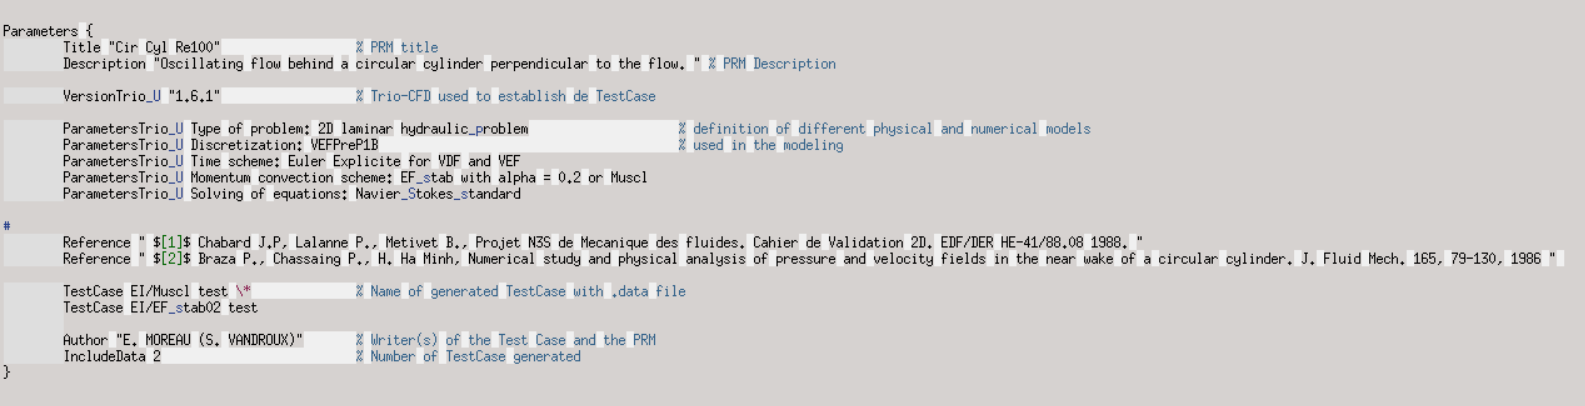
\includegraphics[width=16cm]{tools/parameters_PRM_1.png}\end{center}
\begin{center}\captionof{figure}{Original \texttt{PRM} syntax version - Parameters part}\end{center}

This part generates the first section of the \texttt{PRM} pdf entiteled \textit{1. Introduction} as follows:\newline
\setlength{\columnseprule}{0.5pt}
\begin{multicols}{2}
\begin{flushleft}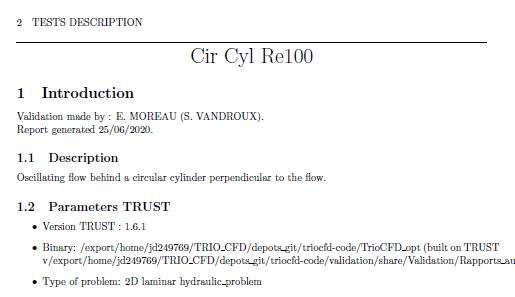
\includegraphics[width=8cm]{tools/parameters_PRM_1_pdf.png}\end{flushleft}
\columnbreak
\vspace{0.5cm}\begin{flushright}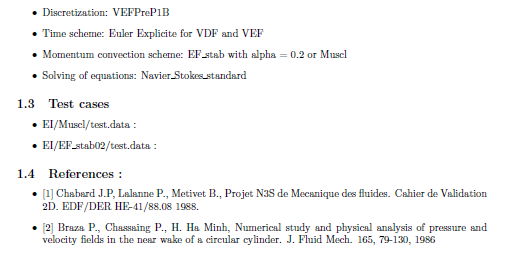
\includegraphics[width=8cm]{tools/parameters_PRM_2_pdf.png}\end{flushright}
\end{multicols}
\begin{center}\captionof{figure}{Original \texttt{PRM} syntax version - Generated introduction}\end{center}

After this first part, chapters can be freely added via the keword \verb"Chapter{ ... }" as follows:\newline
\begin{center}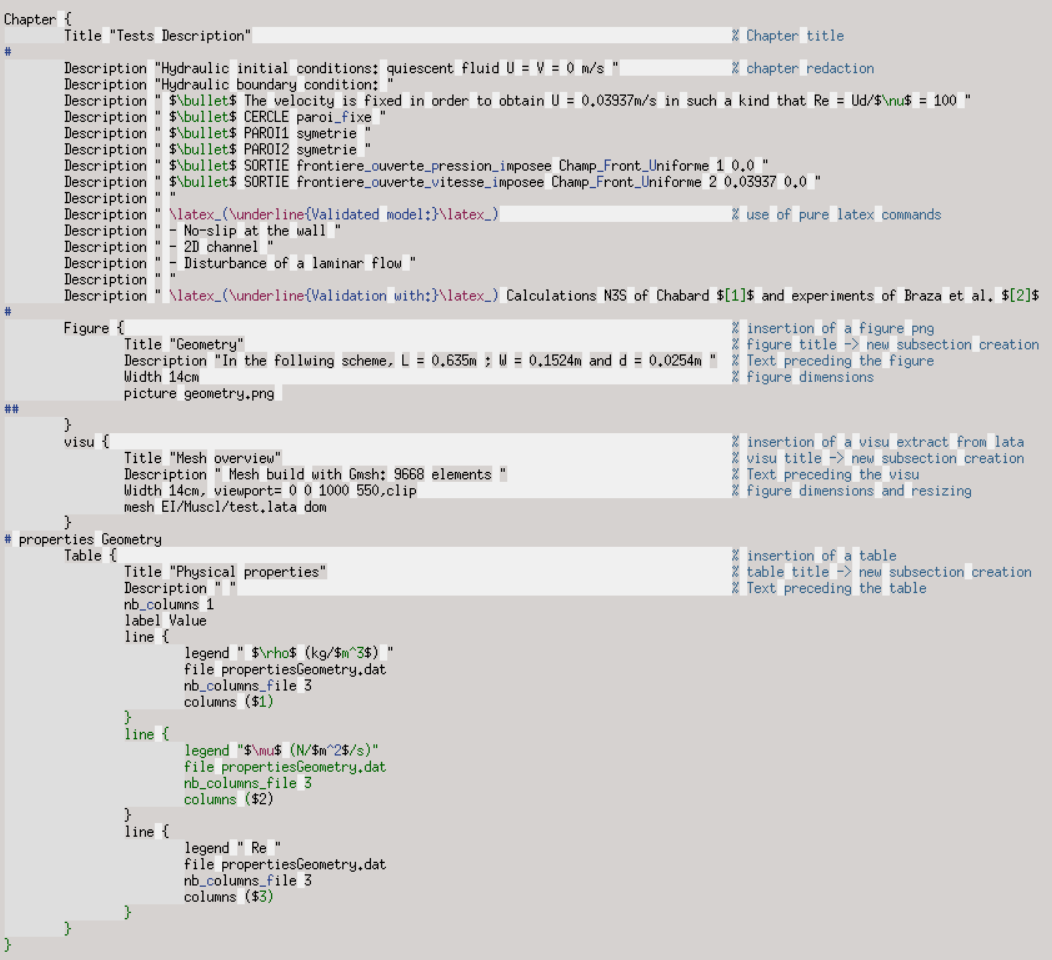
\includegraphics[width=12cm]{tools/chapter_PRM_1.png}\end{center}
\begin{center}\captionof{figure}{Original \texttt{PRM} syntax version - Chapter part}\end{center}

This part generates the second section of the \texttt{PRM} pdf entiteled \textit{2. Tests Description} as follows:\newline
\begin{center}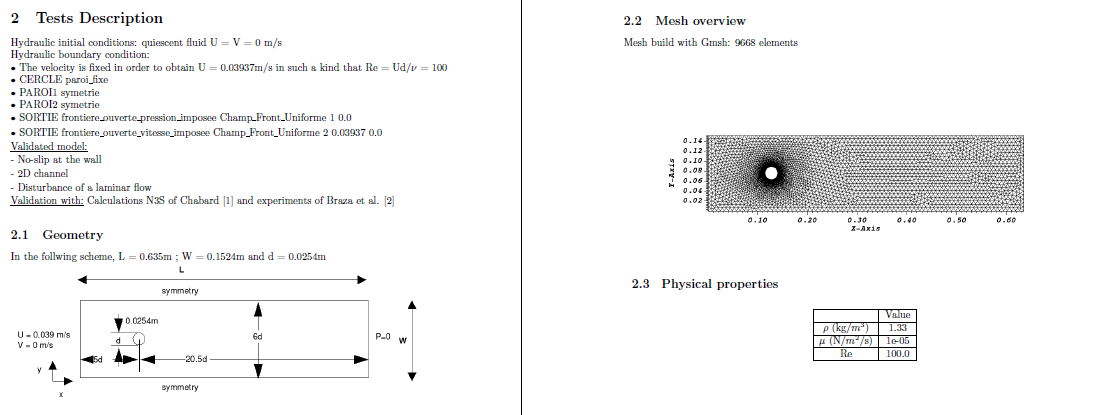
\includegraphics[width=15cm]{tools/chapter_PRM_1_pdf.png}\end{center}
\begin{center}\captionof{figure}{Original \texttt{PRM} syntax version - Generated chapter}\end{center}

%%%%%%%%%%%%%%%%%%%%%%%%%%%%%%%%%%%%%%%%%%%%%%%%%%%%%%%%%%%%%%%%%%%%%%%%%%%%%%%%%%%%%%%%
\section{\label{sec:New-PRM-syntax}New \textsf{PRM} syntax}
\lhead{\textit{New-PRM-syntax}}
\rhead{\textit{METHODOLOGY}}

\subsection{\label{subsec:General-improvements}General improvements}
Improvements have been made to the \texttt{Run\_fiche} procedure (managed
by \texttt{TRUST} code) and a new tag, \texttt{newvalidTrio}, has
been created to activate the new formalism. Some modifications have
been made in this new version for the generation of the \LaTeX~file from
the \texttt{PRM} file, without affecting the syntax of the \texttt{PRM}.
Thus, the \texttt{PRM} still includes the first block of instructions
entitled \texttt{Parameters} (see Section \ref{sec:Old-PRM-syntax})
which is followed by several blocks of instructions entitled by new
tags (or keywords). Those new keywords are listed in Section \ref{subsec:Modification-of-Python}.
The tag \texttt{Chapter} appearing in previous versions is removed and replaced
by many other tags. An additional improvement concerns the ``headers
and footers'' of PDF files. In earlier versions, the left header stated
the number and title of last section whereas the left footer stated
the test name. Now, the name is put on the left header, the left footer
is empty and the right footer still states the page number. That modification
was necessary for the concatenation of \LaTeX~files into one single
document and facilitates the readability.

\subsection{\label{subsec:Modification-of-Python}Modification of \texttt{Python}
script}
As seen in section \ref{sec:Old-PRM-syntax}, adding a new figure,
\texttt{visu}, or \texttt{table} automatically created
a new subsection. The title of that subsection is the same as the
figure name (respectively \texttt{visu} or \texttt{table}). Therefore,
too many irrelevant subsections were created and the title was used
as a caption for figures. In this work, the \texttt{Python} scripts
have been modified so that the title fields of figures (resp. \texttt{visu}
and \texttt{tables}) now correspond to the caption and their creation
no longer generates a subsection.\medskip\newline

\begin{table}[H]
\begin{centering}
	\begin{tabular}{lll}
	\hline 
	\noalign{\vskip0.3cm}
	\textbf{CONTENT OF NEW }\texttt{\textbf{\large{}PRM}}\textbf{ file} & $\qquad$ & \textbf{KEYWORDS OF NEW }\texttt{\textbf{\large{}PRM}}\textbf{ SYNTAX}\tabularnewline[0.2cm]
	\hline
	\noalign{\vskip0.1cm}
	\hline 
	\rowcolor{gray!10}%
	\begin{tabular}{c}
		\tabularnewline
		\textbf{1. Purpose}\tabularnewline
		\end{tabular} &  & %
	\begin{tabular}{lll}
		\textbf{English} &  & \textbf{French}\tabularnewline
		\texttt{\textbf{purpose~~~~~~~}} &  & \texttt{\textbf{objectif}}\tabularnewline
		\end{tabular}\tabularnewline
	\begin{tabular}{l}
		\textbf{2. Problem description}\tabularnewline
		{\small{}~~~~~2.1 Geometry}\tabularnewline
		{\small{}~~~~~2.2 Initial and boundary conditions}\tabularnewline
		{\small{}~~~~~2.3 Fluid properties}\tabularnewline
		{\small{}~~~~~2.4 Flow Physics}\tabularnewline
		\end{tabular} &  & %
	\begin{tabular}{lll}
		\texttt{\textbf{pb\_description}} &  & \tabularnewline
		\texttt{geometry} &  & \texttt{geometrie}\tabularnewline
		\texttt{\textbf{icbc}} &  & \texttt{\textbf{cicl}}\tabularnewline
		\texttt{\textbf{fluidprop}} &  & \texttt{\textbf{propfluide}}\tabularnewline
		\texttt{\textbf{flowphy}} &  & \texttt{\textbf{phyecou}}\tabularnewline
		\end{tabular}\tabularnewline
	\rowcolor{gray!10}%
	\begin{tabular}{l}
		\textbf{3. Case Setup}\tabularnewline
		{\small{}~~~~~3.1 Grid}\tabularnewline
		{\small{}~~~~~3.2 Model options}\tabularnewline
		{\small{}~~~~~3.3 Other options (calculations)}\tabularnewline
		\end{tabular} &  & %
	\begin{tabular}{lll}
		\texttt{\textbf{casesetup}} &  & \texttt{description\_cas}\tabularnewline
		\texttt{grid} &  & \texttt{maillage}\tabularnewline
		\texttt{model\_options~} &  & \texttt{options\_modele}\tabularnewline
		\texttt{other\_options} &  & \texttt{autres\_options}\tabularnewline
		\end{tabular}\tabularnewline
	\begin{tabular}{l}
		\textbf{4. Results}\tabularnewline
		{\small{}~~~~~3.1 Specific information}\tabularnewline
		{\small{}~~~~~3.2 Data plots}\tabularnewline
		\end{tabular} &  & %
	\begin{tabular}{lll}
		\texttt{\textbf{results~~~~~~~}} &  & \texttt{resultats}\tabularnewline
		none &  & \tabularnewline
		none &  & \tabularnewline
		\end{tabular}\tabularnewline
	\rowcolor{gray!10}%
	\begin{tabular}{c}
		\textbf{5. Conclusion}\tabularnewline
		\end{tabular} &  & %
	\begin{tabular}{l}
		\texttt{conclusion}\tabularnewline
	\end{tabular}\tabularnewline
	\begin{tabular}{c}
		\textbf{6. References}\tabularnewline
		\end{tabular} &  & %
	\begin{tabular}{l}
		\texttt{Reference} in block \texttt{\textbf{Parameters}}\tabularnewline
		\end{tabular}\tabularnewline
	\rowcolor{gray!10}%
	\begin{tabular}{c}
		\textbf{7. Datafile}\tabularnewline
		\end{tabular} &  & %
	\begin{tabular}{l}
		\texttt{TestCase} in block \texttt{\textbf{Parameters}} (if followed by \texttt{\textbf{\textbackslash{}{*}}})\tabularnewline
		\end{tabular}\tabularnewline
	\hline 
	\end{tabular}
\par\end{centering}
\end{table}
\begin{center}\captionof{table}{\label{tab:New-PRM-syntax:}New blocks of instructions in \texttt{PRM}
file: content (left) and corresponding keywords (right) in English or French.}.\end{center}

Moreover, the \texttt{PRM} is now interpreted line by line in order to allow better positioning
of the figures in the validation sheet. Previously, the \texttt{Description} fields were
all displayed together at the start of a section/subsection and the figures afterwards.
The \texttt{Python} script has been enhanced with the use of double dictionary to write, 
in the generated \LaTeX~file, the fields in the same order as that of the \texttt{PRM}.
It is therefore now possible to alternate the \texttt{Description}, \texttt{Figure},
\texttt{Visu} or \texttt{Table} fields and their order will be reproduced in the .tex file.\medskip\newline

In addition to these modifications, a new \texttt{PRM} syntax has
been implemented in order to present an identical content for all
validation sheets: now seven sections define all of them. Those sections
are listed in Table \ref{tab:New-PRM-syntax:} (left part). When writing
one \texttt{PRM} file, a new section corresponds to a new block of
instructions which must be declared by its corresponding keyword.
The list of keywords is presented in Table \ref{tab:New-PRM-syntax:}
(right part). All instructions inside the block must be enclosed by
braces: e.g \texttt{objectif \{...\}}, \texttt{pb\_description \{...\}},
\texttt{maillage \{...\}} and so on, where ``\texttt{...}'' means
several instructions on several lines.

Let us remind that in the old \texttt{PRM} syntax, the unique keyword
\texttt{Chapter} was defined as many times as necessary for defining
a new block of instructions. In particular, the number and name of
Sections were chosen by the authors (see Section \ref{sec:Old-PRM-syntax})
and the final rendering was different from one sheet to another.
With the new syntax, the blocks of instructions follow the first one
called \texttt{Parameters}. The second block of instructions is \texttt{objective
\{\}}, the third one is \texttt{pb\_description \{...\}}, and so on
until \texttt{conclusion \{...\}}. The block \texttt{Parameters} 
already existed in previous \texttt{PRM} version but minor modifications
have been brought. The commands are listed in Table \ref{tab:Required-keywords-in}
and an example of use is presented in Alg. \ref{alg:Example-of-use}.
The first one, \texttt{newvalidTrio}, is mandatory because this new
flag indicates the new \texttt{PRM} template. \texttt{TestCase} and
\texttt{ParametersTrio\_U} can be used multiple times in the block. 

\setlength{\tabcolsep}{0.1cm}
\renewcommand{\arraystretch}{1.25}
\begin{table}[H]
\begin{centering}
\begin{tabular}{lll}
\hline 
\textbf{Keywords} & $\qquad$ & \textbf{Use}\tabularnewline
\hline 
\texttt{newvalidTrio} &  & Required keyword to activate the new syntax\tabularnewline
\texttt{Title} &  & Defines title of the validation sheet\tabularnewline
\texttt{VersionTrio\_U} &  & First version of \texttt{TrioCFD} that performed validation\tabularnewline
\texttt{ParametersTrio\_U} &  & Comments that appear in Section 4.1 of the validation sheet\tabularnewline
\texttt{Reference} &  & References cited in the validation sheet\tabularnewline
\texttt{TestCase} &  & List of test cases run by \texttt{TrioCFD} and included in the validation
sheet\tabularnewline
\texttt{Author} &  & First authors who carried out this validation\tabularnewline
\texttt{IncludeData} &  & Command for including the entry datafile of TrioCFD\tabularnewline
\texttt{Description} &  & available in initial formalism, is no longer taken into account.\tabularnewline
\hline 
\end{tabular}
\par\end{centering}
\begin{center}\caption{\label{tab:Required-keywords-in}Keywords that can be used in block
\texttt{Parameters} for \texttt{PRM} files.}\end{center}
\end{table}

~
\begin{center}
\begin{algorithm}[H]
{\footnotesize{}\VerbatimInput{Exemple-Parameters-PRM.txt}}{\footnotesize\par}

\caption{\label{alg:Example-of-use}One example of block \texttt{Parameters}
(for brevity, few instructions are replaced by ``\texttt{...}'').}
\end{algorithm}\end{center}

The keyword \textbf{Description}, available in the inital formalism, is no longer taken into account.\smallskip\newline

In the old formalism, \texttt{Chapter} block was defined as many time as necessary with title chosen by the writer of the validation sheet (see Chapter II.1).
With this new formalism, predefined blocks can be used after the block \texttt{Parameters}.\smallskip\newline
\begin{description}
\item [{The~second~block}] is \texttt{Purpose} which can be activated
by the keyword \texttt{purpose} or \texttt{objectif}. In the PDF file,
the section \textbf{Purpose} is then created provided that the author
wants to fill it up. It explains which models will be validated in
the sheet and what sort of results (numerical, analytical, ...) \texttt{TrioCFD}
will be compared with.\smallskip\newline

\item [{The~third~block}] is \texttt{Problem description} which can be
activated by the keyword \texttt{pb\_description}. The section named
\textbf{Problem description} is then created. In this block, 4 sub-blocks
are available for creating 4 subsections which describe the geometry
of the physical domain defined to model the phenomenon, the initial
and boundary conditions used in the modeling, the fluid properties
and the flow physics. They can be activated with the following keywords:\smallskip\newline
\begin{table}[H]
\begin{centering}
\begin{tabular*}{16cm}{m{4.5cm} m{3cm} m{7.5cm}}
\hline 
\textbf{Keyword} & \textbf{Subsection number} & \textbf{Subsection title}\tabularnewline
\hline 
\textbf{geometry} or \textbf{geometrie} & 2.1 & Geometry\tabularnewline
\textbf{icbc} or \textbf{cicl} & 2.2 & Initial Conditions and Boundary Conditions\tabularnewline
\textbf{fluidprop} or \textbf{propfluide} & 2.3 & Fluid Properties\tabularnewline
\textbf{flowphy} or \textbf{phyecou} & 2.4 & Flow Physics\tabularnewline
\hline 
\end{tabular*}
\par\end{centering}
\caption{\label{tab:List-of-keyword-pbdes}List of keywords for the \texttt{Problem description} block.}
\end{table}

\item [{The~fourth~block}] entitled \texttt{Case Setup} block and activable
by the keyword casesetup or description\_cas has 3 available subsections
which can be defined by:\smallskip\newline
\begin{table}[H]
\begin{centering}
\begin{tabular*}{16cm}{m{4.5cm} m{3cm} m{7.5cm}}
\hline 
\textbf{Keyword} & \textbf{Subsection number} & \textbf{Subsection title}\tabularnewline
\hline 
\textbf{grid\_mesh} or \textbf{maillage} & 3.1 & Grid\tabularnewline
\begin{flushleft}\textbf{model\_options} or \textbf{options\_modele}\end{flushleft} & 3.2 & Model Options\tabularnewline
\begin{flushleft}\textbf{other\_options} or \textbf{autres\_options}\end{flushleft} & 3.3 & Other Options (calculation)\tabularnewline
\hline 
\end{tabular*}
\par\end{centering}
\caption{\label{tab:List-of-keyword-casesetup}List of keywords for the \texttt{Case Setup} block.}
\end{table}

\item [{The~fifth~block}] is an overview of the results of interest from
the validation sheet. This block entitled \textbf{Results} and activable
by the keyword \texttt{results} or \texttt{resultats} is composed
of two subsections. No keyword needed to activate those subsections
and the Results block definition is sufficient to create them.\\
The first, named \textbf{Validation Specific Informations} is automatically
generated and groups the fields \texttt{VersionTrio\_U} and \texttt{ParametersTrio\_U}
defined in the \texttt{Parameters} block. The performance table for
each test case is automatically inserted at the end of this subsection.\\
The second subsection, entitled \textbf{Plot Data} is generated by
reading line by line the keywords \texttt{Description}, \texttt{Figure},
\texttt{Visu} or \texttt{Table} defined by the author in the block.
Respecting this order allows an easier writing and reading of the \texttt{PRM}
file.

\item [{The~last~block}] named \texttt{Conclusion} defined by the keyword
\texttt{conclusion} has no subsection and is filled by line-by-line
reading of the \texttt{PRM} like the other blocks. Here is an assessment
of the validation status of the sheet.

\item [{The~two~last~sections}] of the validation sheet, \textbf{References}
and \textbf{Data Files}, are automatically generated respectively
from keywords \texttt{Reference} and \texttt{TestCase} inside the
\texttt{Parameters} block.\medskip\newline
\end{description}
Four instructions can be used inside all blocks and sub-blocks: \texttt{Description},
\texttt{Figure}, \texttt{Visu} and \texttt{Table} that can be repeated
as many times as necessary and in the desired writing order.

%%%%%%%%%%%%%%%%%%%%%%%%%%%%%%%%%%%%%%%%%%%%%%%%%%%%%%%%%%%%%%%%%%%%%%%%%%%%%%%%%%%%%%%%
%%%%%%%%%%%%%%%%%%%%%%%%%%%%%%%%%%%%%%%%%%%%%%%%%%%%%%%%%%%%%%%%%%%%%%%%%%%%%%%%%%%%%%%%
\chapter{\label{chap:Validation-report-generation}\LaTeX~files and report generation}
\lhead{\textit{\LaTeX~files and report generation}}
\rhead{\textit{METHODOLOGY}}
The procedure for generating this report is flexible and automated.
As a matter of fact, each author can work independently on each validation
sheet with the new \texttt{PRM} template (Section \ref{sec:New-PRM-syntax}).
Moreover, all parts of this document are written in several \LaTeX~files
with clear names (Section \ref{sec:LaTeX_files}). A new one can
easily be added. Finally a shell script automates the following tasks:
gathering all \LaTeX~files, cleaning all sheets texfiles (Section
\ref{sec:Generating-the-report}) and making one single PDF document.
%%%%%%%%%%%%%%%%%%%%%%%%%%%%%%%%%%%%%%%%%%%%%%%%%%%%%%%%%%%%%%%%%%%%%%%%%%%%%%%%%%%%%%%%
\section{\label{sec:LaTeX_files}\LaTeX~files}
\lhead{\textit{\LaTeX~files}}
\rhead{\textit{METHODOLOGY}}
The main \LaTeX~file of this report is named \texttt{validation\_report\_TrioCFD.tex}.
The file contains the standard instructions \texttt{\textbackslash{}documentclass},
\texttt{\textbackslash{}usepackage},\texttt{ \textbackslash{}begin\{document\}}
and \texttt{\textbackslash{}end\{document\}}. The eight parts of this
report are written in eight separated \LaTeX~files (see their names
in Tab. \ref{tab:LaTeX_files}). Those files are included in the main
with the command \texttt{\textbackslash{}input\{\}} (e.g. \texttt{\textbackslash{}input\{./part1-introduction.tex\}}).

\begin{table}[H]
\begin{centering}
\begin{tabular}{ll}
\hline 
\textbf{\LaTeX~file} & \textbf{Comment}\tabularnewline
\hline 
\texttt{validation\_report\_TrioCFD.tex} & Main file\tabularnewline
\texttt{part1-introduction.tex} & File included\tabularnewline
\texttt{part2-methodology.tex} & id\tabularnewline
\texttt{part3-laminar.tex} & id\tabularnewline
\texttt{part4-thermallaminar.tex} & id\tabularnewline
\texttt{part5-turbulent.tex} & id\tabularnewline
\texttt{part6-thermalturbulent.tex} & id\tabularnewline
\texttt{part7-FT.tex} & id\tabularnewline
\texttt{part8-conclusion.tex} & id\tabularnewline
\hline 
\end{tabular}
\par\end{centering}
\caption{\label{tab:LaTeX_files}\LaTeX~files of this report.}
\end{table}

The validation sheets are also included in the main by the same command.
All of them are placed inside the folder \texttt{./fiches} containing
subfolders of all test cases e.g.\texttt{ Poiseuille\_flow\_2D\_VDF\_VEF},\texttt{
Cir\_Cyl\_Re100}, \texttt{OBI\_diffuser\_VEF\_k\_eps}, and so on ...
Inside them, the \LaTeX~file of each validation sheet is called
\texttt{fic.tex} which can be found in the directory \texttt{./build/.tmp/}.
For instance, instruction for including the validation sheet of ``Lid
driven cavity flow'' is:\newline
\texttt{ \textbackslash{}input\{./fiches/Lid\_driven\_cavity/build/.tmp/fic.tex\}}.
All these \texttt{fic.tex} files were generated by \texttt{Python} scripts reading
the \texttt{PRM} template.
%%%%%%%%%%%%%%%%%%%%%%%%%%%%%%%%%%%%%%%%%%%%%%%%%%%%%%%%%%%%%%%%%%%%%%%%%%%%%%%%%%%%%%%%
\section{\label{sec:Generating-the-report}New shell script for gathering all \texttt{.tex} files}
\lhead{\textit{New shell script for gathering all \texttt{.tex} files}}
\rhead{\textit{METHODOLOGY}}
The folder \texttt{fiches} and all subfolders of test cases are created
by \texttt{generer\_rapport\_valid.unix}. For all test cases, the
first task of this shell script is to copy the \texttt{build} directory
of \texttt{TrioCFD} results in corresponding subfolders. The second
task is to clean each \texttt{fic.tex} file in order to be included
in the main \LaTeX~file. Finally the instruction \texttt{pdflatex
validation\_report\_TrioCFD.tex} compiles and generates the PDF file.

%%%%%%%%%%%%%%%%%%%%%%%%%%%%%%%%%%%%%%%%%%%%%%%%%%%%%%%%%%%%%%%%%%%%%%%%%%%%%%%%%%%%%%%%
\section{Enhancement}
\lhead{\textit{Enhancement}}
\rhead{\textit{METHODOLOGY}}
For future versions of this document, the shell script will be enhanced.
Currently, adding a new sheet to the report is carried out manually
in the shell script. It would be more comfortable to automate the
procedure by copying all \texttt{PRM} files which contains the keyword
\texttt{newvalidTrio}, copy the build directory and do a loop inside
the shell script.

%%%%%%%%%%%%%%%%%%%%%%%%%%%%%%%%%%%%%%%%%%%%%%%%%%%%%%%%%%%%%%%%%%%%%%%%%%%%%%%%%%%%%%
\part{Laminar Flow}
\chead{
\tikz[remember picture,overlay] {%
    \fill [LimeGreen,fill opacity=.2]
    ([yshift=0pt]current page header area.south west -| current page.north west)
    rectangle
    (current page.north east)
    ;
    \fill [LimeGreen,fill opacity=.2]
    ([yshift=-45pt]current page.south west)
    rectangle
    (current page footer area.north east -| current page.north east)
    ;
  }
}
\rhead{LAMINAR FLOW}
\normalsize \normalfont
%\baselineskip=16pt
\vspace*{1.5cm}
\lettrine[lines=2,slope=0pt,nindent=4pt]{\textbf{I}}{n} this third part of the document,
the test cases with laminar flows are considered.
Let us remind that a flow is laminar when the viscous forces dominates the inertial ones. 
This competition is characterized by the Reynolds number (Re) which is non-dimensional and
defined as $Re=L U_{0}/\nu$, where $L$ is a characteristic linear dimension, $\nu$
is the kinematic viscosity and $U_{0}$ a characteristic velocity of the system.
A flow characterized by a Reynolds number under a critical value of 2000 (approximately)
is considered as laminar. Beyond this value, the flow is considered as turbulent.
The validation cases of turbulent flows will be considered in Part V of this document. In what
follows, three academic cases are detailed:\vspace*{0.5cm}\newline
\hspace*{0.5cm} $\bullet$ Poiseuille flow\vspace*{0.5cm}\newline
\hspace*{0.5cm} $\bullet$ Lid driven cavity flow\vspace*{0.5cm}\newline
\hspace*{0.5cm} $\bullet$ Cylinder in laminar Cross Flow for Re = 100\vspace*{3cm}\newline
\begin{center}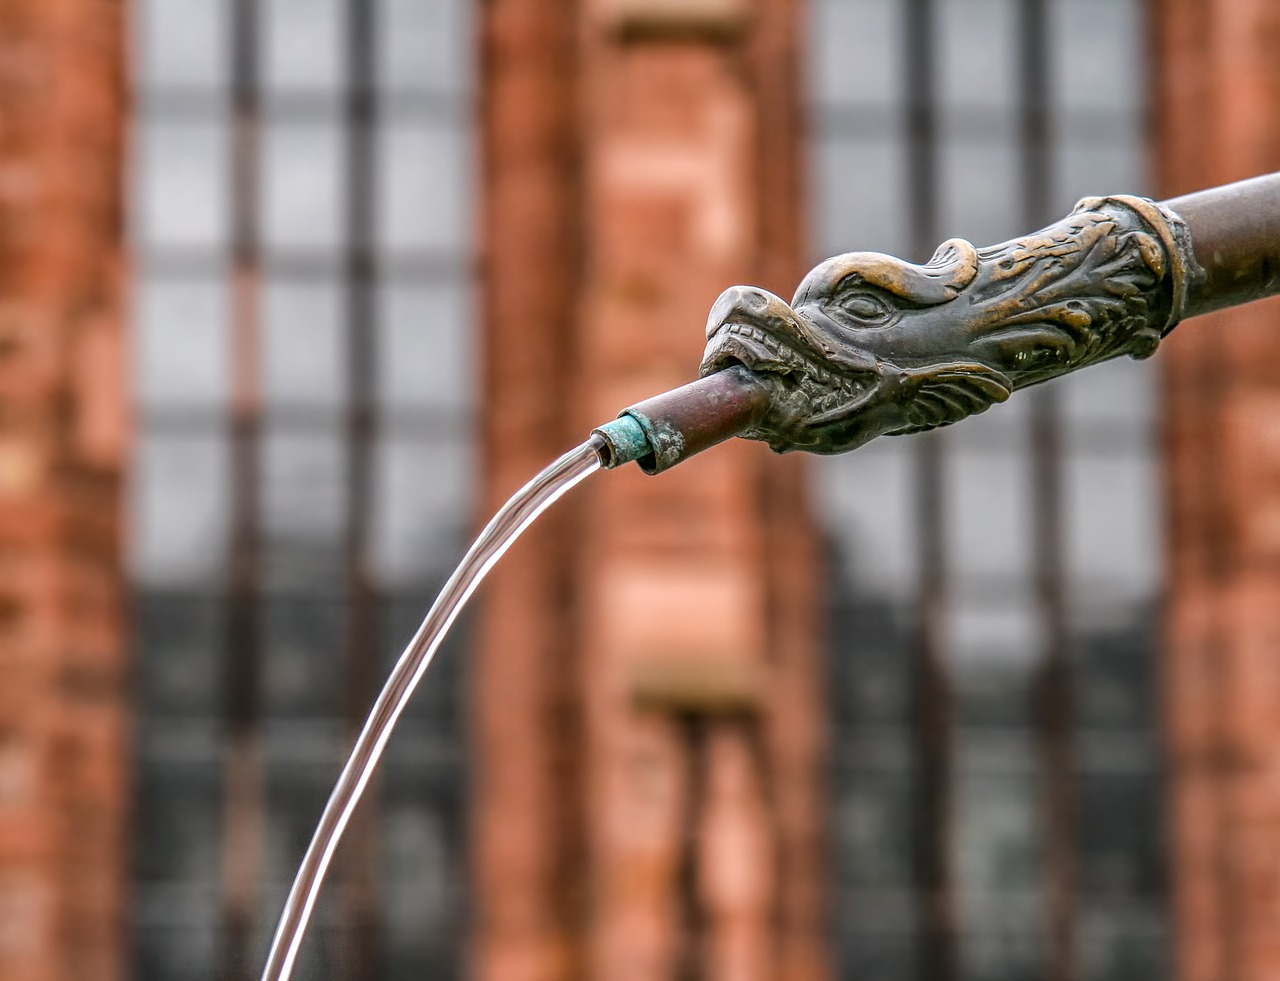
\includegraphics[width=7cm]{tools/jet_laminaire.jpg}\end{center}

\newpage
\chapter{Poiseuille flow 2D with VDF and VEF meshes}
\lhead{Poiseuille flow 2D with VDF and VEF meshes}
\rhead{LAMINAR FLOW}
\def\orig{..}
% This file was generated automaticaly with the genererCources.py script
\documentclass[10pt,twoside,a4paper]{article}
\usepackage[ascii]{}
\usepackage{longtable}
\usepackage[utf8]{inputenc}
% \usepackage[french]{babel}
\usepackage{amsmath,amssymb,amsfonts,textcomp}
\usepackage{color}
% \usepackage{calc}
% \usepackage{hyperref}
% \hypersetup{colorlinks=true, linkcolor=blue, filecolor=blue, pagecolor=blue, urlcolor=blue}
\usepackage{graphicx}
\usepackage{fancyhdr}
% \usepackage[pdfpagemode=FullScreen,bookmarksopen=true,bookmarks=true]{hyperref}
\usepackage[bookmarksopen=true,bookmarks=true]{hyperref}

% \usepackage{verbatim}
%\usepackage{moreverb}
\usepackage{listings}

\setlength\hoffset{0cm}
\setlength\voffset{0cm}
\setlength\oddsidemargin{0cm}
\setlength\evensidemargin{0cm}
\setlength\topmargin{0cm}
\setlength\headheight{1cm}
\setlength\headsep{0.2cm}
\setlength\marginparsep{0cm}
\setlength\marginparwidth{0cm}
\setlength\footskip{2cm}
\setlength\textwidth{16cm}
\setlength{\parindent}{0pt}

% Style page
\renewcommand{\sectionmark}[1]{\markboth{#1}{#1}}
\pagestyle{fancy}
\lhead{\leftmark\\\rightmark}
\chead{}
\rhead{}
%\lfoot{\textit{Genere automatiquement avec genererCourbe.py, v0.1.}}
\lfoot{\textit{ Validation du fonctionnement du forcage spectral en presence de bulles.}}
\cfoot{}
\rfoot{\thepage}
\renewcommand{\headrulewidth}{0.4pt}
\renewcommand{\footrulewidth}{0.4pt}

\title{Validation du fonctionnement du forcage spectral en presence de bulles.}
\author{Gabriel Ramirez}
\date{02/09/2021}

\makeindex

% Debut document
\begin{document}
{\huge\centering Validation du fonctionnement du forcage spectral en presence de bulles. \par}

\section{Introduction}

Validation made by : Gabriel Ramirez.\\Report generated  02/09/2021.
\par\subsection{Description}

\par\subsection{Parameters TRUST }
\begin{itemize}
\item Version TRUST : 1.8.2
\end{itemize}
\par\subsection{Test cases}
\begin{itemize}
\item ADV\_X00/RUN00/spec\_bulles\_point2.data : \textit{}
\item NO\_ADV\_X00/RUN00/spec\_bulles\_point2.data : \textit{}
\item ADV\_0X0/RUN00/spec\_bulles\_point2.data : \textit{}
\item NO\_ADV\_0X0/RUN00/spec\_bulles\_point2.data : \textit{}
\item ADV\_010/RUN00/spec\_bulles\_point2.data : \textit{}
\item NO\_ADV\_010/RUN00/spec\_bulles\_point2.data : \textit{}
\item ADV\_001/RUN00/spec\_bulles\_point2.data : \textit{}
\item NO\_ADV\_001/RUN00/spec\_bulles\_point2.data : \textit{}
\item ADV\_101/RUN00/spec\_bulles\_point2.data : \textit{}
\item NO\_ADV\_101/RUN00/spec\_bulles\_point2.data : \textit{}
\end{itemize}

% Debut Chapitre
\section{Purpose}
Valider l'advection du champ de force. 

% Debut Chapitre
\section{Description du probl\`{e}me}
Le texte n'est pas a jour du tout. La suite de g\'{e}nr\'{e}rateur al\'{e}atoires se trouve dans .../OUT/random...out.
On impose un champ de force dans le domaine. Le champs de force est donn\'{e} par les \'{e}quations suivantes : 
 $F_{ph} = \mathcal{TF}(b(k,t_{i+1}) - \frac{k(k \cdot b(k, t_{i+1}))}{k \cdot k})$ 
$ b(k,t_{i+1}) = b(k,t_i)(1-\frac{\Delta t}{T_L}) + e_i(k,t) (2\sigma^2 \frac{\Delta t}{T_L})^{1/2}$
Le domaine est un cube de c\^{o}t\'{e} 01, allant de -0.005 a  0.005.
Chaque face est p\'{e}riodique
La viscosit\'{e} cin\'{e}matique est fix\'{e}e \`{a} 3.0128062836164946e-07 . La masse volumique \`{a} 1171.3. Il n'y a pas de phase gazeuse.


% Debut Chapitre
\section{Description du cas}
Le domaine est discr\'{e}tis\'{e} en $128^3$ \'{e}l\'{e}ments tous de m\^{e}me taille.

 On dispose quatre segments de relev\'{e} align\'{e}s selon X, quatre segments selon Y et 4 segments selon Z. 

% Debut Chapitre
\section{R\'{e}sultats}
On montre ici la visualitation des champs de la force spectrale ajout\'{e}e,
 obtenus avec l'outil de visualisation visit .


Force spectrale, avec reprises
 obtenus avec l'outil de visualisation visit .


Forces spectrales, obtenues d'une traite
 obtenus avec l'outil de visualisation visit .


Les marques correspondent aux premiers relev\'{e}s tels que l'autocorr\'{e}lation soit nulle ou n\'{e}gative.
     


% Debut Chapitre
\section{Conclusion}
En conclusion, on n'observe pas d'abh\'{e}rrance

% Debut Chapitre
\section{Computer performance}


% Debut tableau




% Fin du document
\end{document}

\newpage
\chapter{2D Lid driven cavity test}
\lhead{2D Lid driven cavity test}
\rhead{LAMINAR FLOW}
\def\orig{..}
% This file was generated automaticaly with the genererCources.py script
\documentclass[10pt,twoside,a4paper]{article}
\usepackage[ascii]{}
\usepackage{longtable}
\usepackage[utf8]{inputenc}
% \usepackage[french]{babel}
\usepackage{amsmath,amssymb,amsfonts,textcomp}
\usepackage{color}
% \usepackage{calc}
% \usepackage{hyperref}
% \hypersetup{colorlinks=true, linkcolor=blue, filecolor=blue, pagecolor=blue, urlcolor=blue}
\usepackage{graphicx}
\usepackage{fancyhdr}
% \usepackage[pdfpagemode=FullScreen,bookmarksopen=true,bookmarks=true]{hyperref}
\usepackage[bookmarksopen=true,bookmarks=true]{hyperref}

% \usepackage{verbatim}
%\usepackage{moreverb}
\usepackage{listings}

\setlength\hoffset{0cm}
\setlength\voffset{0cm}
\setlength\oddsidemargin{0cm}
\setlength\evensidemargin{0cm}
\setlength\topmargin{0cm}
\setlength\headheight{1cm}
\setlength\headsep{0.2cm}
\setlength\marginparsep{0cm}
\setlength\marginparwidth{0cm}
\setlength\footskip{2cm}
\setlength\textwidth{16cm}
\setlength{\parindent}{0pt}

% Style page
\renewcommand{\sectionmark}[1]{\markboth{#1}{#1}}
\pagestyle{fancy}
\lhead{\leftmark\\\rightmark}
\chead{}
\rhead{}
%\lfoot{\textit{Genere automatiquement avec genererCourbe.py, v0.1.}}
\lfoot{\textit{ Validation du fonctionnement du forcage spectral en presence de bulles.}}
\cfoot{}
\rfoot{\thepage}
\renewcommand{\headrulewidth}{0.4pt}
\renewcommand{\footrulewidth}{0.4pt}

\title{Validation du fonctionnement du forcage spectral en presence de bulles.}
\author{Gabriel Ramirez}
\date{02/09/2021}

\makeindex

% Debut document
\begin{document}
{\huge\centering Validation du fonctionnement du forcage spectral en presence de bulles. \par}

\section{Introduction}

Validation made by : Gabriel Ramirez.\\Report generated  02/09/2021.
\par\subsection{Description}

\par\subsection{Parameters TRUST }
\begin{itemize}
\item Version TRUST : 1.8.2
\end{itemize}
\par\subsection{Test cases}
\begin{itemize}
\item ADV\_X00/RUN00/spec\_bulles\_point2.data : \textit{}
\item NO\_ADV\_X00/RUN00/spec\_bulles\_point2.data : \textit{}
\item ADV\_0X0/RUN00/spec\_bulles\_point2.data : \textit{}
\item NO\_ADV\_0X0/RUN00/spec\_bulles\_point2.data : \textit{}
\item ADV\_010/RUN00/spec\_bulles\_point2.data : \textit{}
\item NO\_ADV\_010/RUN00/spec\_bulles\_point2.data : \textit{}
\item ADV\_001/RUN00/spec\_bulles\_point2.data : \textit{}
\item NO\_ADV\_001/RUN00/spec\_bulles\_point2.data : \textit{}
\item ADV\_101/RUN00/spec\_bulles\_point2.data : \textit{}
\item NO\_ADV\_101/RUN00/spec\_bulles\_point2.data : \textit{}
\end{itemize}

% Debut Chapitre
\section{Purpose}
Valider l'advection du champ de force. 

% Debut Chapitre
\section{Description du probl\`{e}me}
Le texte n'est pas a jour du tout. La suite de g\'{e}nr\'{e}rateur al\'{e}atoires se trouve dans .../OUT/random...out.
On impose un champ de force dans le domaine. Le champs de force est donn\'{e} par les \'{e}quations suivantes : 
 $F_{ph} = \mathcal{TF}(b(k,t_{i+1}) - \frac{k(k \cdot b(k, t_{i+1}))}{k \cdot k})$ 
$ b(k,t_{i+1}) = b(k,t_i)(1-\frac{\Delta t}{T_L}) + e_i(k,t) (2\sigma^2 \frac{\Delta t}{T_L})^{1/2}$
Le domaine est un cube de c\^{o}t\'{e} 01, allant de -0.005 a  0.005.
Chaque face est p\'{e}riodique
La viscosit\'{e} cin\'{e}matique est fix\'{e}e \`{a} 3.0128062836164946e-07 . La masse volumique \`{a} 1171.3. Il n'y a pas de phase gazeuse.


% Debut Chapitre
\section{Description du cas}
Le domaine est discr\'{e}tis\'{e} en $128^3$ \'{e}l\'{e}ments tous de m\^{e}me taille.

 On dispose quatre segments de relev\'{e} align\'{e}s selon X, quatre segments selon Y et 4 segments selon Z. 

% Debut Chapitre
\section{R\'{e}sultats}
On montre ici la visualitation des champs de la force spectrale ajout\'{e}e,
 obtenus avec l'outil de visualisation visit .


Force spectrale, avec reprises
 obtenus avec l'outil de visualisation visit .


Forces spectrales, obtenues d'une traite
 obtenus avec l'outil de visualisation visit .


Les marques correspondent aux premiers relev\'{e}s tels que l'autocorr\'{e}lation soit nulle ou n\'{e}gative.
     


% Debut Chapitre
\section{Conclusion}
En conclusion, on n'observe pas d'abh\'{e}rrance

% Debut Chapitre
\section{Computer performance}


% Debut tableau




% Fin du document
\end{document}

\newpage
\chapter{Cylinder in Laminar Cross Flow}
\lhead{Cylinder in Laminar Cross Flow - Cir Cyl Re100}
\rhead{LAMINAR FLOW}
\def\orig{..}
% This file was generated automaticaly with the genererCources.py script
\documentclass[10pt,twoside,a4paper]{article}
\usepackage[ascii]{}
\usepackage{longtable}
\usepackage[utf8]{inputenc}
% \usepackage[french]{babel}
\usepackage{amsmath,amssymb,amsfonts,textcomp}
\usepackage{color}
% \usepackage{calc}
% \usepackage{hyperref}
% \hypersetup{colorlinks=true, linkcolor=blue, filecolor=blue, pagecolor=blue, urlcolor=blue}
\usepackage{graphicx}
\usepackage{fancyhdr}
% \usepackage[pdfpagemode=FullScreen,bookmarksopen=true,bookmarks=true]{hyperref}
\usepackage[bookmarksopen=true,bookmarks=true]{hyperref}

% \usepackage{verbatim}
%\usepackage{moreverb}
\usepackage{listings}

\setlength\hoffset{0cm}
\setlength\voffset{0cm}
\setlength\oddsidemargin{0cm}
\setlength\evensidemargin{0cm}
\setlength\topmargin{0cm}
\setlength\headheight{1cm}
\setlength\headsep{0.2cm}
\setlength\marginparsep{0cm}
\setlength\marginparwidth{0cm}
\setlength\footskip{2cm}
\setlength\textwidth{16cm}
\setlength{\parindent}{0pt}

% Style page
\renewcommand{\sectionmark}[1]{\markboth{#1}{#1}}
\pagestyle{fancy}
\lhead{\leftmark\\\rightmark}
\chead{}
\rhead{}
%\lfoot{\textit{Genere automatiquement avec genererCourbe.py, v0.1.}}
\lfoot{\textit{ Validation du fonctionnement du forcage spectral en presence de bulles.}}
\cfoot{}
\rfoot{\thepage}
\renewcommand{\headrulewidth}{0.4pt}
\renewcommand{\footrulewidth}{0.4pt}

\title{Validation du fonctionnement du forcage spectral en presence de bulles.}
\author{Gabriel Ramirez}
\date{02/09/2021}

\makeindex

% Debut document
\begin{document}
{\huge\centering Validation du fonctionnement du forcage spectral en presence de bulles. \par}

\section{Introduction}

Validation made by : Gabriel Ramirez.\\Report generated  02/09/2021.
\par\subsection{Description}

\par\subsection{Parameters TRUST }
\begin{itemize}
\item Version TRUST : 1.8.2
\end{itemize}
\par\subsection{Test cases}
\begin{itemize}
\item ADV\_X00/RUN00/spec\_bulles\_point2.data : \textit{}
\item NO\_ADV\_X00/RUN00/spec\_bulles\_point2.data : \textit{}
\item ADV\_0X0/RUN00/spec\_bulles\_point2.data : \textit{}
\item NO\_ADV\_0X0/RUN00/spec\_bulles\_point2.data : \textit{}
\item ADV\_010/RUN00/spec\_bulles\_point2.data : \textit{}
\item NO\_ADV\_010/RUN00/spec\_bulles\_point2.data : \textit{}
\item ADV\_001/RUN00/spec\_bulles\_point2.data : \textit{}
\item NO\_ADV\_001/RUN00/spec\_bulles\_point2.data : \textit{}
\item ADV\_101/RUN00/spec\_bulles\_point2.data : \textit{}
\item NO\_ADV\_101/RUN00/spec\_bulles\_point2.data : \textit{}
\end{itemize}

% Debut Chapitre
\section{Purpose}
Valider l'advection du champ de force. 

% Debut Chapitre
\section{Description du probl\`{e}me}
Le texte n'est pas a jour du tout. La suite de g\'{e}nr\'{e}rateur al\'{e}atoires se trouve dans .../OUT/random...out.
On impose un champ de force dans le domaine. Le champs de force est donn\'{e} par les \'{e}quations suivantes : 
 $F_{ph} = \mathcal{TF}(b(k,t_{i+1}) - \frac{k(k \cdot b(k, t_{i+1}))}{k \cdot k})$ 
$ b(k,t_{i+1}) = b(k,t_i)(1-\frac{\Delta t}{T_L}) + e_i(k,t) (2\sigma^2 \frac{\Delta t}{T_L})^{1/2}$
Le domaine est un cube de c\^{o}t\'{e} 01, allant de -0.005 a  0.005.
Chaque face est p\'{e}riodique
La viscosit\'{e} cin\'{e}matique est fix\'{e}e \`{a} 3.0128062836164946e-07 . La masse volumique \`{a} 1171.3. Il n'y a pas de phase gazeuse.


% Debut Chapitre
\section{Description du cas}
Le domaine est discr\'{e}tis\'{e} en $128^3$ \'{e}l\'{e}ments tous de m\^{e}me taille.

 On dispose quatre segments de relev\'{e} align\'{e}s selon X, quatre segments selon Y et 4 segments selon Z. 

% Debut Chapitre
\section{R\'{e}sultats}
On montre ici la visualitation des champs de la force spectrale ajout\'{e}e,
 obtenus avec l'outil de visualisation visit .


Force spectrale, avec reprises
 obtenus avec l'outil de visualisation visit .


Forces spectrales, obtenues d'une traite
 obtenus avec l'outil de visualisation visit .


Les marques correspondent aux premiers relev\'{e}s tels que l'autocorr\'{e}lation soit nulle ou n\'{e}gative.
     


% Debut Chapitre
\section{Conclusion}
En conclusion, on n'observe pas d'abh\'{e}rrance

% Debut Chapitre
\section{Computer performance}


% Debut tableau




% Fin du document
\end{document}

%%%%%%%%%%%%%%%%%%%%%%%%%%%%%%%%%%%%%%%%%%%%%%%%%%%%%%%%%%%%%%%%%%%%%%%%%%%%%%%%%%%%%%
\part{Thermal Laminar Flow}
%\markright{THERMAL LAMINAR FLOW}
\chead{
\tikz[remember picture,overlay] {%
    \fill [ForestGreen,fill opacity=.2]
    ([yshift=0pt]current page header area.south west -| current page.north west)
    rectangle
    (current page.north east)
    ;
    \fill [ForestGreen,fill opacity=.2]
    ([yshift=-45pt]current page.south west)
    rectangle
    (current page footer area.north east -| current page.north east)
    ;
  }
}
\rhead{THERMAL LAMINAR FLOW}
\normalsize \normalfont
\lettrine[lines=2,slope=0pt,nindent=4pt]{\textbf{C}}{ompared} to the previous part, the phenomena considered here will
involve thermal aspects and, in particular, the flow is still laminar.\newline
The first validation sheet of this category corresponds to the \textbf{Vahl Davis} benchmark, which is one of the
most known test case for checking the coupling between the convective and thermal phenomena.
The second one \textbf{Oscillatory convection flow} is very similar to the Vahl Davis test case but this time,
the cavity and therefore the flow are no longer symmetrical.
\vspace*{3cm}\newline
\begin{center}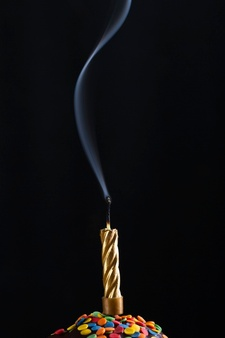
\includegraphics[width=7cm]{tools/bougie.png}\end{center}

\newpage
\chapter{Convection Vahl Davis}
\markboth{Convection Vahl Davis}{}
\def\orig{..}
% This file was generated automaticaly with the genererCources.py script
\documentclass[10pt,twoside,a4paper]{article}
\usepackage[ascii]{}
\usepackage{longtable}
\usepackage[utf8]{inputenc}
% \usepackage[french]{babel}
\usepackage{amsmath,amssymb,amsfonts,textcomp}
\usepackage{color}
% \usepackage{calc}
% \usepackage{hyperref}
% \hypersetup{colorlinks=true, linkcolor=blue, filecolor=blue, pagecolor=blue, urlcolor=blue}
\usepackage{graphicx}
\usepackage{fancyhdr}
% \usepackage[pdfpagemode=FullScreen,bookmarksopen=true,bookmarks=true]{hyperref}
\usepackage[bookmarksopen=true,bookmarks=true]{hyperref}

% \usepackage{verbatim}
%\usepackage{moreverb}
\usepackage{listings}

\setlength\hoffset{0cm}
\setlength\voffset{0cm}
\setlength\oddsidemargin{0cm}
\setlength\evensidemargin{0cm}
\setlength\topmargin{0cm}
\setlength\headheight{1cm}
\setlength\headsep{0.2cm}
\setlength\marginparsep{0cm}
\setlength\marginparwidth{0cm}
\setlength\footskip{2cm}
\setlength\textwidth{16cm}
\setlength{\parindent}{0pt}

% Style page
\renewcommand{\sectionmark}[1]{\markboth{#1}{#1}}
\pagestyle{fancy}
\lhead{\leftmark\\\rightmark}
\chead{}
\rhead{}
%\lfoot{\textit{Genere automatiquement avec genererCourbe.py, v0.1.}}
\lfoot{\textit{ Validation du fonctionnement du forcage spectral en presence de bulles.}}
\cfoot{}
\rfoot{\thepage}
\renewcommand{\headrulewidth}{0.4pt}
\renewcommand{\footrulewidth}{0.4pt}

\title{Validation du fonctionnement du forcage spectral en presence de bulles.}
\author{Gabriel Ramirez}
\date{02/09/2021}

\makeindex

% Debut document
\begin{document}
{\huge\centering Validation du fonctionnement du forcage spectral en presence de bulles. \par}

\section{Introduction}

Validation made by : Gabriel Ramirez.\\Report generated  02/09/2021.
\par\subsection{Description}

\par\subsection{Parameters TRUST }
\begin{itemize}
\item Version TRUST : 1.8.2
\end{itemize}
\par\subsection{Test cases}
\begin{itemize}
\item ADV\_X00/RUN00/spec\_bulles\_point2.data : \textit{}
\item NO\_ADV\_X00/RUN00/spec\_bulles\_point2.data : \textit{}
\item ADV\_0X0/RUN00/spec\_bulles\_point2.data : \textit{}
\item NO\_ADV\_0X0/RUN00/spec\_bulles\_point2.data : \textit{}
\item ADV\_010/RUN00/spec\_bulles\_point2.data : \textit{}
\item NO\_ADV\_010/RUN00/spec\_bulles\_point2.data : \textit{}
\item ADV\_001/RUN00/spec\_bulles\_point2.data : \textit{}
\item NO\_ADV\_001/RUN00/spec\_bulles\_point2.data : \textit{}
\item ADV\_101/RUN00/spec\_bulles\_point2.data : \textit{}
\item NO\_ADV\_101/RUN00/spec\_bulles\_point2.data : \textit{}
\end{itemize}

% Debut Chapitre
\section{Purpose}
Valider l'advection du champ de force. 

% Debut Chapitre
\section{Description du probl\`{e}me}
Le texte n'est pas a jour du tout. La suite de g\'{e}nr\'{e}rateur al\'{e}atoires se trouve dans .../OUT/random...out.
On impose un champ de force dans le domaine. Le champs de force est donn\'{e} par les \'{e}quations suivantes : 
 $F_{ph} = \mathcal{TF}(b(k,t_{i+1}) - \frac{k(k \cdot b(k, t_{i+1}))}{k \cdot k})$ 
$ b(k,t_{i+1}) = b(k,t_i)(1-\frac{\Delta t}{T_L}) + e_i(k,t) (2\sigma^2 \frac{\Delta t}{T_L})^{1/2}$
Le domaine est un cube de c\^{o}t\'{e} 01, allant de -0.005 a  0.005.
Chaque face est p\'{e}riodique
La viscosit\'{e} cin\'{e}matique est fix\'{e}e \`{a} 3.0128062836164946e-07 . La masse volumique \`{a} 1171.3. Il n'y a pas de phase gazeuse.


% Debut Chapitre
\section{Description du cas}
Le domaine est discr\'{e}tis\'{e} en $128^3$ \'{e}l\'{e}ments tous de m\^{e}me taille.

 On dispose quatre segments de relev\'{e} align\'{e}s selon X, quatre segments selon Y et 4 segments selon Z. 

% Debut Chapitre
\section{R\'{e}sultats}
On montre ici la visualitation des champs de la force spectrale ajout\'{e}e,
 obtenus avec l'outil de visualisation visit .


Force spectrale, avec reprises
 obtenus avec l'outil de visualisation visit .


Forces spectrales, obtenues d'une traite
 obtenus avec l'outil de visualisation visit .


Les marques correspondent aux premiers relev\'{e}s tels que l'autocorr\'{e}lation soit nulle ou n\'{e}gative.
     


% Debut Chapitre
\section{Conclusion}
En conclusion, on n'observe pas d'abh\'{e}rrance

% Debut Chapitre
\section{Computer performance}


% Debut tableau




% Fin du document
\end{document}

\newpage
\chapter{Oscillatory convection flow}
\markboth{Oscillatory convection flow}{}
\def\orig{..}
% This file was generated automaticaly with the genererCources.py script
\documentclass[10pt,twoside,a4paper]{article}
\usepackage[ascii]{}
\usepackage{longtable}
\usepackage[utf8]{inputenc}
% \usepackage[french]{babel}
\usepackage{amsmath,amssymb,amsfonts,textcomp}
\usepackage{color}
% \usepackage{calc}
% \usepackage{hyperref}
% \hypersetup{colorlinks=true, linkcolor=blue, filecolor=blue, pagecolor=blue, urlcolor=blue}
\usepackage{graphicx}
\usepackage{fancyhdr}
% \usepackage[pdfpagemode=FullScreen,bookmarksopen=true,bookmarks=true]{hyperref}
\usepackage[bookmarksopen=true,bookmarks=true]{hyperref}

% \usepackage{verbatim}
%\usepackage{moreverb}
\usepackage{listings}

\setlength\hoffset{0cm}
\setlength\voffset{0cm}
\setlength\oddsidemargin{0cm}
\setlength\evensidemargin{0cm}
\setlength\topmargin{0cm}
\setlength\headheight{1cm}
\setlength\headsep{0.2cm}
\setlength\marginparsep{0cm}
\setlength\marginparwidth{0cm}
\setlength\footskip{2cm}
\setlength\textwidth{16cm}
\setlength{\parindent}{0pt}

% Style page
\renewcommand{\sectionmark}[1]{\markboth{#1}{#1}}
\pagestyle{fancy}
\lhead{\leftmark\\\rightmark}
\chead{}
\rhead{}
%\lfoot{\textit{Genere automatiquement avec genererCourbe.py, v0.1.}}
\lfoot{\textit{ Validation du fonctionnement du forcage spectral en presence de bulles.}}
\cfoot{}
\rfoot{\thepage}
\renewcommand{\headrulewidth}{0.4pt}
\renewcommand{\footrulewidth}{0.4pt}

\title{Validation du fonctionnement du forcage spectral en presence de bulles.}
\author{Gabriel Ramirez}
\date{02/09/2021}

\makeindex

% Debut document
\begin{document}
{\huge\centering Validation du fonctionnement du forcage spectral en presence de bulles. \par}

\section{Introduction}

Validation made by : Gabriel Ramirez.\\Report generated  02/09/2021.
\par\subsection{Description}

\par\subsection{Parameters TRUST }
\begin{itemize}
\item Version TRUST : 1.8.2
\end{itemize}
\par\subsection{Test cases}
\begin{itemize}
\item ADV\_X00/RUN00/spec\_bulles\_point2.data : \textit{}
\item NO\_ADV\_X00/RUN00/spec\_bulles\_point2.data : \textit{}
\item ADV\_0X0/RUN00/spec\_bulles\_point2.data : \textit{}
\item NO\_ADV\_0X0/RUN00/spec\_bulles\_point2.data : \textit{}
\item ADV\_010/RUN00/spec\_bulles\_point2.data : \textit{}
\item NO\_ADV\_010/RUN00/spec\_bulles\_point2.data : \textit{}
\item ADV\_001/RUN00/spec\_bulles\_point2.data : \textit{}
\item NO\_ADV\_001/RUN00/spec\_bulles\_point2.data : \textit{}
\item ADV\_101/RUN00/spec\_bulles\_point2.data : \textit{}
\item NO\_ADV\_101/RUN00/spec\_bulles\_point2.data : \textit{}
\end{itemize}

% Debut Chapitre
\section{Purpose}
Valider l'advection du champ de force. 

% Debut Chapitre
\section{Description du probl\`{e}me}
Le texte n'est pas a jour du tout. La suite de g\'{e}nr\'{e}rateur al\'{e}atoires se trouve dans .../OUT/random...out.
On impose un champ de force dans le domaine. Le champs de force est donn\'{e} par les \'{e}quations suivantes : 
 $F_{ph} = \mathcal{TF}(b(k,t_{i+1}) - \frac{k(k \cdot b(k, t_{i+1}))}{k \cdot k})$ 
$ b(k,t_{i+1}) = b(k,t_i)(1-\frac{\Delta t}{T_L}) + e_i(k,t) (2\sigma^2 \frac{\Delta t}{T_L})^{1/2}$
Le domaine est un cube de c\^{o}t\'{e} 01, allant de -0.005 a  0.005.
Chaque face est p\'{e}riodique
La viscosit\'{e} cin\'{e}matique est fix\'{e}e \`{a} 3.0128062836164946e-07 . La masse volumique \`{a} 1171.3. Il n'y a pas de phase gazeuse.


% Debut Chapitre
\section{Description du cas}
Le domaine est discr\'{e}tis\'{e} en $128^3$ \'{e}l\'{e}ments tous de m\^{e}me taille.

 On dispose quatre segments de relev\'{e} align\'{e}s selon X, quatre segments selon Y et 4 segments selon Z. 

% Debut Chapitre
\section{R\'{e}sultats}
On montre ici la visualitation des champs de la force spectrale ajout\'{e}e,
 obtenus avec l'outil de visualisation visit .


Force spectrale, avec reprises
 obtenus avec l'outil de visualisation visit .


Forces spectrales, obtenues d'une traite
 obtenus avec l'outil de visualisation visit .


Les marques correspondent aux premiers relev\'{e}s tels que l'autocorr\'{e}lation soit nulle ou n\'{e}gative.
     


% Debut Chapitre
\section{Conclusion}
En conclusion, on n'observe pas d'abh\'{e}rrance

% Debut Chapitre
\section{Computer performance}


% Debut tableau




% Fin du document
\end{document}

%%%%%%%%%%%%%%%%%%%%%%%%%%%%%%%%%%%%%%%%%%%%%%%%%%%%%%%%%%%%%%%%%%%%%%%%%%%%%%%%%%%%%%
\part{Turbulent Flow}
\markright{TURBULENT FLOW}
\chead{
\tikz[remember picture,overlay] {%
    \fill [SkyBlue,fill opacity=.2]
    ([yshift=0pt]current page header area.south west -| current page.north west)
    rectangle
    (current page.north east)
    ;
    \fill [SkyBlue,fill opacity=.2]
    ([yshift=-45pt]current page.south west)
    rectangle
    (current page footer area.north east -| current page.north east)
    ;
  }
}
\normalsize \normalfont
\lettrine[lines=2,slope=0pt,nindent=4pt]{\textbf{I}}{n} this fifth part of the document,
the flow pattern changes completely compared to the two previous parts since here are considered turbulent flows.
Let us remind that a flow is considered as turbulent when the Reynolds number is greater than 2000.
This critical Reynolds number corresponds to the moment when the viscous forces are no longer strong enough
to absorb the vortices. Fluid motion is characterized by chaotic changes in pressure and flow velocity.
The flow has a whirlpool character at all points: eddies whose size, location and orientation vary constantly.
Turbulent flows are therefore characterized by a very disordered appearance, behavior that is difficult to predict,
and the existence of numerous space and time scales.\newline
In this version of the report, two cases are studied:\vspace*{0.3cm}\newline
\hspace*{0.5cm} $\bullet$ Turbulent flow in a 2D diffuser with the $k-\epsilon$ model\vspace*{0.3cm}\newline
\hspace*{0.5cm} $\bullet$ Mixing length in 2D and 3D VEF-plane channel\vspace*{0.3cm}\newline
This part will be enriched in a following version with, in particular, a case in 3D.\vspace*{2cm}\newline
\begin{center}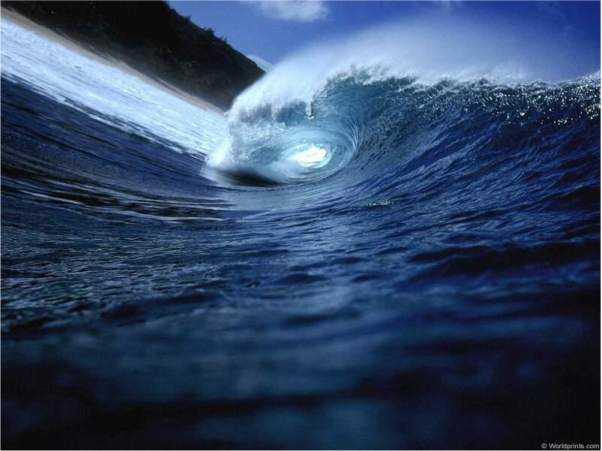
\includegraphics[width=12cm]{tools/mer_turb.png}\end{center}

\newpage
\chapter{Turbulent flow in a 2D diffuser with the $k-\epsilon$ model}
\markboth{Turbulent flow in a 2D diffuser with the $k-\epsilon$ model}{}
\def\orig{..}
% This file was generated automaticaly with the genererCources.py script
\documentclass[10pt,twoside,a4paper]{article}
\usepackage[ascii]{}
\usepackage{longtable}
\usepackage[utf8]{inputenc}
% \usepackage[french]{babel}
\usepackage{amsmath,amssymb,amsfonts,textcomp}
\usepackage{color}
% \usepackage{calc}
% \usepackage{hyperref}
% \hypersetup{colorlinks=true, linkcolor=blue, filecolor=blue, pagecolor=blue, urlcolor=blue}
\usepackage{graphicx}
\usepackage{fancyhdr}
% \usepackage[pdfpagemode=FullScreen,bookmarksopen=true,bookmarks=true]{hyperref}
\usepackage[bookmarksopen=true,bookmarks=true]{hyperref}

% \usepackage{verbatim}
%\usepackage{moreverb}
\usepackage{listings}

\setlength\hoffset{0cm}
\setlength\voffset{0cm}
\setlength\oddsidemargin{0cm}
\setlength\evensidemargin{0cm}
\setlength\topmargin{0cm}
\setlength\headheight{1cm}
\setlength\headsep{0.2cm}
\setlength\marginparsep{0cm}
\setlength\marginparwidth{0cm}
\setlength\footskip{2cm}
\setlength\textwidth{16cm}
\setlength{\parindent}{0pt}

% Style page
\renewcommand{\sectionmark}[1]{\markboth{#1}{#1}}
\pagestyle{fancy}
\lhead{\leftmark\\\rightmark}
\chead{}
\rhead{}
%\lfoot{\textit{Genere automatiquement avec genererCourbe.py, v0.1.}}
\lfoot{\textit{ Validation du fonctionnement du forcage spectral en presence de bulles.}}
\cfoot{}
\rfoot{\thepage}
\renewcommand{\headrulewidth}{0.4pt}
\renewcommand{\footrulewidth}{0.4pt}

\title{Validation du fonctionnement du forcage spectral en presence de bulles.}
\author{Gabriel Ramirez}
\date{02/09/2021}

\makeindex

% Debut document
\begin{document}
{\huge\centering Validation du fonctionnement du forcage spectral en presence de bulles. \par}

\section{Introduction}

Validation made by : Gabriel Ramirez.\\Report generated  02/09/2021.
\par\subsection{Description}

\par\subsection{Parameters TRUST }
\begin{itemize}
\item Version TRUST : 1.8.2
\end{itemize}
\par\subsection{Test cases}
\begin{itemize}
\item ADV\_X00/RUN00/spec\_bulles\_point2.data : \textit{}
\item NO\_ADV\_X00/RUN00/spec\_bulles\_point2.data : \textit{}
\item ADV\_0X0/RUN00/spec\_bulles\_point2.data : \textit{}
\item NO\_ADV\_0X0/RUN00/spec\_bulles\_point2.data : \textit{}
\item ADV\_010/RUN00/spec\_bulles\_point2.data : \textit{}
\item NO\_ADV\_010/RUN00/spec\_bulles\_point2.data : \textit{}
\item ADV\_001/RUN00/spec\_bulles\_point2.data : \textit{}
\item NO\_ADV\_001/RUN00/spec\_bulles\_point2.data : \textit{}
\item ADV\_101/RUN00/spec\_bulles\_point2.data : \textit{}
\item NO\_ADV\_101/RUN00/spec\_bulles\_point2.data : \textit{}
\end{itemize}

% Debut Chapitre
\section{Purpose}
Valider l'advection du champ de force. 

% Debut Chapitre
\section{Description du probl\`{e}me}
Le texte n'est pas a jour du tout. La suite de g\'{e}nr\'{e}rateur al\'{e}atoires se trouve dans .../OUT/random...out.
On impose un champ de force dans le domaine. Le champs de force est donn\'{e} par les \'{e}quations suivantes : 
 $F_{ph} = \mathcal{TF}(b(k,t_{i+1}) - \frac{k(k \cdot b(k, t_{i+1}))}{k \cdot k})$ 
$ b(k,t_{i+1}) = b(k,t_i)(1-\frac{\Delta t}{T_L}) + e_i(k,t) (2\sigma^2 \frac{\Delta t}{T_L})^{1/2}$
Le domaine est un cube de c\^{o}t\'{e} 01, allant de -0.005 a  0.005.
Chaque face est p\'{e}riodique
La viscosit\'{e} cin\'{e}matique est fix\'{e}e \`{a} 3.0128062836164946e-07 . La masse volumique \`{a} 1171.3. Il n'y a pas de phase gazeuse.


% Debut Chapitre
\section{Description du cas}
Le domaine est discr\'{e}tis\'{e} en $128^3$ \'{e}l\'{e}ments tous de m\^{e}me taille.

 On dispose quatre segments de relev\'{e} align\'{e}s selon X, quatre segments selon Y et 4 segments selon Z. 

% Debut Chapitre
\section{R\'{e}sultats}
On montre ici la visualitation des champs de la force spectrale ajout\'{e}e,
 obtenus avec l'outil de visualisation visit .


Force spectrale, avec reprises
 obtenus avec l'outil de visualisation visit .


Forces spectrales, obtenues d'une traite
 obtenus avec l'outil de visualisation visit .


Les marques correspondent aux premiers relev\'{e}s tels que l'autocorr\'{e}lation soit nulle ou n\'{e}gative.
     


% Debut Chapitre
\section{Conclusion}
En conclusion, on n'observe pas d'abh\'{e}rrance

% Debut Chapitre
\section{Computer performance}


% Debut tableau




% Fin du document
\end{document}

\newpage
\chapter{Mixing length in 2D and 3D VEF-plane channel}
\markboth{Mixing length in 2D and 3D VEF-plane channel}{}
\def\orig{..}
% This file was generated automaticaly with the genererCources.py script
\documentclass[10pt,twoside,a4paper]{article}
\usepackage[ascii]{}
\usepackage{longtable}
\usepackage[utf8]{inputenc}
% \usepackage[french]{babel}
\usepackage{amsmath,amssymb,amsfonts,textcomp}
\usepackage{color}
% \usepackage{calc}
% \usepackage{hyperref}
% \hypersetup{colorlinks=true, linkcolor=blue, filecolor=blue, pagecolor=blue, urlcolor=blue}
\usepackage{graphicx}
\usepackage{fancyhdr}
% \usepackage[pdfpagemode=FullScreen,bookmarksopen=true,bookmarks=true]{hyperref}
\usepackage[bookmarksopen=true,bookmarks=true]{hyperref}

% \usepackage{verbatim}
%\usepackage{moreverb}
\usepackage{listings}

\setlength\hoffset{0cm}
\setlength\voffset{0cm}
\setlength\oddsidemargin{0cm}
\setlength\evensidemargin{0cm}
\setlength\topmargin{0cm}
\setlength\headheight{1cm}
\setlength\headsep{0.2cm}
\setlength\marginparsep{0cm}
\setlength\marginparwidth{0cm}
\setlength\footskip{2cm}
\setlength\textwidth{16cm}
\setlength{\parindent}{0pt}

% Style page
\renewcommand{\sectionmark}[1]{\markboth{#1}{#1}}
\pagestyle{fancy}
\lhead{\leftmark\\\rightmark}
\chead{}
\rhead{}
%\lfoot{\textit{Genere automatiquement avec genererCourbe.py, v0.1.}}
\lfoot{\textit{ Validation du fonctionnement du forcage spectral en presence de bulles.}}
\cfoot{}
\rfoot{\thepage}
\renewcommand{\headrulewidth}{0.4pt}
\renewcommand{\footrulewidth}{0.4pt}

\title{Validation du fonctionnement du forcage spectral en presence de bulles.}
\author{Gabriel Ramirez}
\date{02/09/2021}

\makeindex

% Debut document
\begin{document}
{\huge\centering Validation du fonctionnement du forcage spectral en presence de bulles. \par}

\section{Introduction}

Validation made by : Gabriel Ramirez.\\Report generated  02/09/2021.
\par\subsection{Description}

\par\subsection{Parameters TRUST }
\begin{itemize}
\item Version TRUST : 1.8.2
\end{itemize}
\par\subsection{Test cases}
\begin{itemize}
\item ADV\_X00/RUN00/spec\_bulles\_point2.data : \textit{}
\item NO\_ADV\_X00/RUN00/spec\_bulles\_point2.data : \textit{}
\item ADV\_0X0/RUN00/spec\_bulles\_point2.data : \textit{}
\item NO\_ADV\_0X0/RUN00/spec\_bulles\_point2.data : \textit{}
\item ADV\_010/RUN00/spec\_bulles\_point2.data : \textit{}
\item NO\_ADV\_010/RUN00/spec\_bulles\_point2.data : \textit{}
\item ADV\_001/RUN00/spec\_bulles\_point2.data : \textit{}
\item NO\_ADV\_001/RUN00/spec\_bulles\_point2.data : \textit{}
\item ADV\_101/RUN00/spec\_bulles\_point2.data : \textit{}
\item NO\_ADV\_101/RUN00/spec\_bulles\_point2.data : \textit{}
\end{itemize}

% Debut Chapitre
\section{Purpose}
Valider l'advection du champ de force. 

% Debut Chapitre
\section{Description du probl\`{e}me}
Le texte n'est pas a jour du tout. La suite de g\'{e}nr\'{e}rateur al\'{e}atoires se trouve dans .../OUT/random...out.
On impose un champ de force dans le domaine. Le champs de force est donn\'{e} par les \'{e}quations suivantes : 
 $F_{ph} = \mathcal{TF}(b(k,t_{i+1}) - \frac{k(k \cdot b(k, t_{i+1}))}{k \cdot k})$ 
$ b(k,t_{i+1}) = b(k,t_i)(1-\frac{\Delta t}{T_L}) + e_i(k,t) (2\sigma^2 \frac{\Delta t}{T_L})^{1/2}$
Le domaine est un cube de c\^{o}t\'{e} 01, allant de -0.005 a  0.005.
Chaque face est p\'{e}riodique
La viscosit\'{e} cin\'{e}matique est fix\'{e}e \`{a} 3.0128062836164946e-07 . La masse volumique \`{a} 1171.3. Il n'y a pas de phase gazeuse.


% Debut Chapitre
\section{Description du cas}
Le domaine est discr\'{e}tis\'{e} en $128^3$ \'{e}l\'{e}ments tous de m\^{e}me taille.

 On dispose quatre segments de relev\'{e} align\'{e}s selon X, quatre segments selon Y et 4 segments selon Z. 

% Debut Chapitre
\section{R\'{e}sultats}
On montre ici la visualitation des champs de la force spectrale ajout\'{e}e,
 obtenus avec l'outil de visualisation visit .


Force spectrale, avec reprises
 obtenus avec l'outil de visualisation visit .


Forces spectrales, obtenues d'une traite
 obtenus avec l'outil de visualisation visit .


Les marques correspondent aux premiers relev\'{e}s tels que l'autocorr\'{e}lation soit nulle ou n\'{e}gative.
     


% Debut Chapitre
\section{Conclusion}
En conclusion, on n'observe pas d'abh\'{e}rrance

% Debut Chapitre
\section{Computer performance}


% Debut tableau




% Fin du document
\end{document}

%%%%%%%%%%%%%%%%%%%%%%%%%%%%%%%%%%%%%%%%%%%%%%%%%%%%%%%%%%%%%%%%%%%%%%%%%%%%%%%%%%%%%%
\part{Thermal Turbulent Flow}
\markright{THERMAL TURBULENT FLOW}
\chead{
\tikz[remember picture,overlay] {%
    \fill [Blue,fill opacity=.2]
    ([yshift=0pt]current page header area.south west -| current page.north west)
    rectangle
    (current page.north east)
    ;
    \fill [Blue,fill opacity=.2]
    ([yshift=-45pt]current page.south west)
    rectangle
    (current page footer area.north east -| current page.north east)
    ;
  }
}
\normalsize \normalfont
\lettrine[lines=2,slope=0pt,nindent=4pt]{\textbf{L}}{ike} for laminar flows, in this section,
thermal aspects are added to turbulent flows.
In this version of the report, two cases are studied:\vspace*{0.3cm}\newline
\hspace*{0.5cm} $\bullet$ Thermal stratification flow in a plenum\vspace*{0.3cm}\newline
\hspace*{0.5cm} $\bullet$ Turbulent flow inside a double-periodic plane channel with heated walls\vspace*{0.3cm}\newline
These two cases both use $k-\epsilon$ model for turbulence and 3D modeling.\vspace*{2cm}\newline
\begin{center}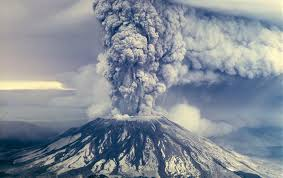
\includegraphics[width=12cm]{tools/volcan.png}\end{center}

%\newpage
%\chapter{Thermal stratification flow in a plenum}
%\markboth{Thermal stratification flow in a plenum}{}
%\def\orig{..}
% This file was generated automaticaly with the genererCources.py script
\documentclass[10pt,twoside,a4paper]{article}
\usepackage[ascii]{}
\usepackage{longtable}
\usepackage[utf8]{inputenc}
% \usepackage[french]{babel}
\usepackage{amsmath,amssymb,amsfonts,textcomp}
\usepackage{color}
% \usepackage{calc}
% \usepackage{hyperref}
% \hypersetup{colorlinks=true, linkcolor=blue, filecolor=blue, pagecolor=blue, urlcolor=blue}
\usepackage{graphicx}
\usepackage{fancyhdr}
% \usepackage[pdfpagemode=FullScreen,bookmarksopen=true,bookmarks=true]{hyperref}
\usepackage[bookmarksopen=true,bookmarks=true]{hyperref}

% \usepackage{verbatim}
%\usepackage{moreverb}
\usepackage{listings}

\setlength\hoffset{0cm}
\setlength\voffset{0cm}
\setlength\oddsidemargin{0cm}
\setlength\evensidemargin{0cm}
\setlength\topmargin{0cm}
\setlength\headheight{1cm}
\setlength\headsep{0.2cm}
\setlength\marginparsep{0cm}
\setlength\marginparwidth{0cm}
\setlength\footskip{2cm}
\setlength\textwidth{16cm}
\setlength{\parindent}{0pt}

% Style page
\renewcommand{\sectionmark}[1]{\markboth{#1}{#1}}
\pagestyle{fancy}
\lhead{\leftmark\\\rightmark}
\chead{}
\rhead{}
%\lfoot{\textit{Genere automatiquement avec genererCourbe.py, v0.1.}}
\lfoot{\textit{ Validation du fonctionnement du forcage spectral en presence de bulles.}}
\cfoot{}
\rfoot{\thepage}
\renewcommand{\headrulewidth}{0.4pt}
\renewcommand{\footrulewidth}{0.4pt}

\title{Validation du fonctionnement du forcage spectral en presence de bulles.}
\author{Gabriel Ramirez}
\date{02/09/2021}

\makeindex

% Debut document
\begin{document}
{\huge\centering Validation du fonctionnement du forcage spectral en presence de bulles. \par}

\section{Introduction}

Validation made by : Gabriel Ramirez.\\Report generated  02/09/2021.
\par\subsection{Description}

\par\subsection{Parameters TRUST }
\begin{itemize}
\item Version TRUST : 1.8.2
\end{itemize}
\par\subsection{Test cases}
\begin{itemize}
\item ADV\_X00/RUN00/spec\_bulles\_point2.data : \textit{}
\item NO\_ADV\_X00/RUN00/spec\_bulles\_point2.data : \textit{}
\item ADV\_0X0/RUN00/spec\_bulles\_point2.data : \textit{}
\item NO\_ADV\_0X0/RUN00/spec\_bulles\_point2.data : \textit{}
\item ADV\_010/RUN00/spec\_bulles\_point2.data : \textit{}
\item NO\_ADV\_010/RUN00/spec\_bulles\_point2.data : \textit{}
\item ADV\_001/RUN00/spec\_bulles\_point2.data : \textit{}
\item NO\_ADV\_001/RUN00/spec\_bulles\_point2.data : \textit{}
\item ADV\_101/RUN00/spec\_bulles\_point2.data : \textit{}
\item NO\_ADV\_101/RUN00/spec\_bulles\_point2.data : \textit{}
\end{itemize}

% Debut Chapitre
\section{Purpose}
Valider l'advection du champ de force. 

% Debut Chapitre
\section{Description du probl\`{e}me}
Le texte n'est pas a jour du tout. La suite de g\'{e}nr\'{e}rateur al\'{e}atoires se trouve dans .../OUT/random...out.
On impose un champ de force dans le domaine. Le champs de force est donn\'{e} par les \'{e}quations suivantes : 
 $F_{ph} = \mathcal{TF}(b(k,t_{i+1}) - \frac{k(k \cdot b(k, t_{i+1}))}{k \cdot k})$ 
$ b(k,t_{i+1}) = b(k,t_i)(1-\frac{\Delta t}{T_L}) + e_i(k,t) (2\sigma^2 \frac{\Delta t}{T_L})^{1/2}$
Le domaine est un cube de c\^{o}t\'{e} 01, allant de -0.005 a  0.005.
Chaque face est p\'{e}riodique
La viscosit\'{e} cin\'{e}matique est fix\'{e}e \`{a} 3.0128062836164946e-07 . La masse volumique \`{a} 1171.3. Il n'y a pas de phase gazeuse.


% Debut Chapitre
\section{Description du cas}
Le domaine est discr\'{e}tis\'{e} en $128^3$ \'{e}l\'{e}ments tous de m\^{e}me taille.

 On dispose quatre segments de relev\'{e} align\'{e}s selon X, quatre segments selon Y et 4 segments selon Z. 

% Debut Chapitre
\section{R\'{e}sultats}
On montre ici la visualitation des champs de la force spectrale ajout\'{e}e,
 obtenus avec l'outil de visualisation visit .


Force spectrale, avec reprises
 obtenus avec l'outil de visualisation visit .


Forces spectrales, obtenues d'une traite
 obtenus avec l'outil de visualisation visit .


Les marques correspondent aux premiers relev\'{e}s tels que l'autocorr\'{e}lation soit nulle ou n\'{e}gative.
     


% Debut Chapitre
\section{Conclusion}
En conclusion, on n'observe pas d'abh\'{e}rrance

% Debut Chapitre
\section{Computer performance}


% Debut tableau




% Fin du document
\end{document}

\newpage
\chapter{Turbulent flow inside a double-periodic plane channel with heated walls}
\markboth{Turbulent flow inside a double-periodic plane channel with heated walls}{}
\def\orig{..}
% This file was generated automaticaly with the genererCources.py script
\documentclass[10pt,twoside,a4paper]{article}
\usepackage[ascii]{}
\usepackage{longtable}
\usepackage[utf8]{inputenc}
% \usepackage[french]{babel}
\usepackage{amsmath,amssymb,amsfonts,textcomp}
\usepackage{color}
% \usepackage{calc}
% \usepackage{hyperref}
% \hypersetup{colorlinks=true, linkcolor=blue, filecolor=blue, pagecolor=blue, urlcolor=blue}
\usepackage{graphicx}
\usepackage{fancyhdr}
% \usepackage[pdfpagemode=FullScreen,bookmarksopen=true,bookmarks=true]{hyperref}
\usepackage[bookmarksopen=true,bookmarks=true]{hyperref}

% \usepackage{verbatim}
%\usepackage{moreverb}
\usepackage{listings}

\setlength\hoffset{0cm}
\setlength\voffset{0cm}
\setlength\oddsidemargin{0cm}
\setlength\evensidemargin{0cm}
\setlength\topmargin{0cm}
\setlength\headheight{1cm}
\setlength\headsep{0.2cm}
\setlength\marginparsep{0cm}
\setlength\marginparwidth{0cm}
\setlength\footskip{2cm}
\setlength\textwidth{16cm}
\setlength{\parindent}{0pt}

% Style page
\renewcommand{\sectionmark}[1]{\markboth{#1}{#1}}
\pagestyle{fancy}
\lhead{\leftmark\\\rightmark}
\chead{}
\rhead{}
%\lfoot{\textit{Genere automatiquement avec genererCourbe.py, v0.1.}}
\lfoot{\textit{ Validation du fonctionnement du forcage spectral en presence de bulles.}}
\cfoot{}
\rfoot{\thepage}
\renewcommand{\headrulewidth}{0.4pt}
\renewcommand{\footrulewidth}{0.4pt}

\title{Validation du fonctionnement du forcage spectral en presence de bulles.}
\author{Gabriel Ramirez}
\date{02/09/2021}

\makeindex

% Debut document
\begin{document}
{\huge\centering Validation du fonctionnement du forcage spectral en presence de bulles. \par}

\section{Introduction}

Validation made by : Gabriel Ramirez.\\Report generated  02/09/2021.
\par\subsection{Description}

\par\subsection{Parameters TRUST }
\begin{itemize}
\item Version TRUST : 1.8.2
\end{itemize}
\par\subsection{Test cases}
\begin{itemize}
\item ADV\_X00/RUN00/spec\_bulles\_point2.data : \textit{}
\item NO\_ADV\_X00/RUN00/spec\_bulles\_point2.data : \textit{}
\item ADV\_0X0/RUN00/spec\_bulles\_point2.data : \textit{}
\item NO\_ADV\_0X0/RUN00/spec\_bulles\_point2.data : \textit{}
\item ADV\_010/RUN00/spec\_bulles\_point2.data : \textit{}
\item NO\_ADV\_010/RUN00/spec\_bulles\_point2.data : \textit{}
\item ADV\_001/RUN00/spec\_bulles\_point2.data : \textit{}
\item NO\_ADV\_001/RUN00/spec\_bulles\_point2.data : \textit{}
\item ADV\_101/RUN00/spec\_bulles\_point2.data : \textit{}
\item NO\_ADV\_101/RUN00/spec\_bulles\_point2.data : \textit{}
\end{itemize}

% Debut Chapitre
\section{Purpose}
Valider l'advection du champ de force. 

% Debut Chapitre
\section{Description du probl\`{e}me}
Le texte n'est pas a jour du tout. La suite de g\'{e}nr\'{e}rateur al\'{e}atoires se trouve dans .../OUT/random...out.
On impose un champ de force dans le domaine. Le champs de force est donn\'{e} par les \'{e}quations suivantes : 
 $F_{ph} = \mathcal{TF}(b(k,t_{i+1}) - \frac{k(k \cdot b(k, t_{i+1}))}{k \cdot k})$ 
$ b(k,t_{i+1}) = b(k,t_i)(1-\frac{\Delta t}{T_L}) + e_i(k,t) (2\sigma^2 \frac{\Delta t}{T_L})^{1/2}$
Le domaine est un cube de c\^{o}t\'{e} 01, allant de -0.005 a  0.005.
Chaque face est p\'{e}riodique
La viscosit\'{e} cin\'{e}matique est fix\'{e}e \`{a} 3.0128062836164946e-07 . La masse volumique \`{a} 1171.3. Il n'y a pas de phase gazeuse.


% Debut Chapitre
\section{Description du cas}
Le domaine est discr\'{e}tis\'{e} en $128^3$ \'{e}l\'{e}ments tous de m\^{e}me taille.

 On dispose quatre segments de relev\'{e} align\'{e}s selon X, quatre segments selon Y et 4 segments selon Z. 

% Debut Chapitre
\section{R\'{e}sultats}
On montre ici la visualitation des champs de la force spectrale ajout\'{e}e,
 obtenus avec l'outil de visualisation visit .


Force spectrale, avec reprises
 obtenus avec l'outil de visualisation visit .


Forces spectrales, obtenues d'une traite
 obtenus avec l'outil de visualisation visit .


Les marques correspondent aux premiers relev\'{e}s tels que l'autocorr\'{e}lation soit nulle ou n\'{e}gative.
     


% Debut Chapitre
\section{Conclusion}
En conclusion, on n'observe pas d'abh\'{e}rrance

% Debut Chapitre
\section{Computer performance}


% Debut tableau




% Fin du document
\end{document}

%%%%%%%%%%%%%%%%%%%%%%%%%%%%%%%%%%%%%%%%%%%%%%%%%%%%%%%%%%%%%%%%%%%%%%%%%%%%%%%%%%%%%%
\part{Two-phase Flows with Front-Tracking}
\markright{TWO-PHASE FLOWS WITH FRONT-TRACKING}
\chead{
\tikz[remember picture,overlay] {%
    \fill [Orchid,fill opacity=.2]
    ([yshift=0pt]current page header area.south west -| current page.north west)
    rectangle
    (current page.north east)
    ;
    \fill [Orchid,fill opacity=.2]
    ([yshift=-45pt]current page.south west)
    rectangle
    (current page footer area.north east -| current page.north east)
    ;
  }
}
\normalsize \normalfont
\lettrine[lines=2,slope=0pt,nindent=4pt]{\textbf{I}}{n} this last part, the test cases correspond to two-phase flows at
local scale. Direct numerical simulations of such flows consist in
modeling two incompressible and immiscible fluids separated by a mobile
interface. The mass and impulsion balance equations hold for each
bulk phase with the viscosity and density of each fluid. The temperature
equation is neglected as well as phase change but the gravity is considered.
In such an approach, bubbles or drops are described individually with
their surface tension and the main difficulty is to follow accurately
interfaces that evolve in space and time. Several numerical methods
are dedicated to such interface tracking. They can be gathered into
two main families: ``diffuse interface method'' and ``sharp interface
method''. In \texttt{TrioCFD}, interfaces are tracked by ``Front-Tracking'',
a sharp interface method, for which the surface of separation between
both fluids is discretized by an additional lagrangian mesh. A re-meshing
is required during the calculation with a fine adjustment of numerical
parameters. In this part, the method is used for simulating problems
of \textbf{oscillating bubble} and \textbf{hanging drop}.\vspace*{3cm} \newline
\begin{center}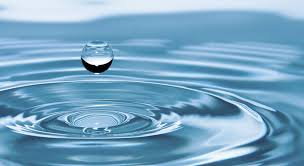
\includegraphics[width=12cm]{tools/goutte.png}\end{center}

\newpage
\chapter{Oscillation of a bubble}
\markboth{Oscillation of a bubble}{}
\def\orig{..}
% This file was generated automaticaly with the genererCources.py script
\documentclass[10pt,twoside,a4paper]{article}
\usepackage[ascii]{}
\usepackage{longtable}
\usepackage[utf8]{inputenc}
% \usepackage[french]{babel}
\usepackage{amsmath,amssymb,amsfonts,textcomp}
\usepackage{color}
% \usepackage{calc}
% \usepackage{hyperref}
% \hypersetup{colorlinks=true, linkcolor=blue, filecolor=blue, pagecolor=blue, urlcolor=blue}
\usepackage{graphicx}
\usepackage{fancyhdr}
% \usepackage[pdfpagemode=FullScreen,bookmarksopen=true,bookmarks=true]{hyperref}
\usepackage[bookmarksopen=true,bookmarks=true]{hyperref}

% \usepackage{verbatim}
%\usepackage{moreverb}
\usepackage{listings}

\setlength\hoffset{0cm}
\setlength\voffset{0cm}
\setlength\oddsidemargin{0cm}
\setlength\evensidemargin{0cm}
\setlength\topmargin{0cm}
\setlength\headheight{1cm}
\setlength\headsep{0.2cm}
\setlength\marginparsep{0cm}
\setlength\marginparwidth{0cm}
\setlength\footskip{2cm}
\setlength\textwidth{16cm}
\setlength{\parindent}{0pt}

% Style page
\renewcommand{\sectionmark}[1]{\markboth{#1}{#1}}
\pagestyle{fancy}
\lhead{\leftmark\\\rightmark}
\chead{}
\rhead{}
%\lfoot{\textit{Genere automatiquement avec genererCourbe.py, v0.1.}}
\lfoot{\textit{ Validation du fonctionnement du forcage spectral en presence de bulles.}}
\cfoot{}
\rfoot{\thepage}
\renewcommand{\headrulewidth}{0.4pt}
\renewcommand{\footrulewidth}{0.4pt}

\title{Validation du fonctionnement du forcage spectral en presence de bulles.}
\author{Gabriel Ramirez}
\date{02/09/2021}

\makeindex

% Debut document
\begin{document}
{\huge\centering Validation du fonctionnement du forcage spectral en presence de bulles. \par}

\section{Introduction}

Validation made by : Gabriel Ramirez.\\Report generated  02/09/2021.
\par\subsection{Description}

\par\subsection{Parameters TRUST }
\begin{itemize}
\item Version TRUST : 1.8.2
\end{itemize}
\par\subsection{Test cases}
\begin{itemize}
\item ADV\_X00/RUN00/spec\_bulles\_point2.data : \textit{}
\item NO\_ADV\_X00/RUN00/spec\_bulles\_point2.data : \textit{}
\item ADV\_0X0/RUN00/spec\_bulles\_point2.data : \textit{}
\item NO\_ADV\_0X0/RUN00/spec\_bulles\_point2.data : \textit{}
\item ADV\_010/RUN00/spec\_bulles\_point2.data : \textit{}
\item NO\_ADV\_010/RUN00/spec\_bulles\_point2.data : \textit{}
\item ADV\_001/RUN00/spec\_bulles\_point2.data : \textit{}
\item NO\_ADV\_001/RUN00/spec\_bulles\_point2.data : \textit{}
\item ADV\_101/RUN00/spec\_bulles\_point2.data : \textit{}
\item NO\_ADV\_101/RUN00/spec\_bulles\_point2.data : \textit{}
\end{itemize}

% Debut Chapitre
\section{Purpose}
Valider l'advection du champ de force. 

% Debut Chapitre
\section{Description du probl\`{e}me}
Le texte n'est pas a jour du tout. La suite de g\'{e}nr\'{e}rateur al\'{e}atoires se trouve dans .../OUT/random...out.
On impose un champ de force dans le domaine. Le champs de force est donn\'{e} par les \'{e}quations suivantes : 
 $F_{ph} = \mathcal{TF}(b(k,t_{i+1}) - \frac{k(k \cdot b(k, t_{i+1}))}{k \cdot k})$ 
$ b(k,t_{i+1}) = b(k,t_i)(1-\frac{\Delta t}{T_L}) + e_i(k,t) (2\sigma^2 \frac{\Delta t}{T_L})^{1/2}$
Le domaine est un cube de c\^{o}t\'{e} 01, allant de -0.005 a  0.005.
Chaque face est p\'{e}riodique
La viscosit\'{e} cin\'{e}matique est fix\'{e}e \`{a} 3.0128062836164946e-07 . La masse volumique \`{a} 1171.3. Il n'y a pas de phase gazeuse.


% Debut Chapitre
\section{Description du cas}
Le domaine est discr\'{e}tis\'{e} en $128^3$ \'{e}l\'{e}ments tous de m\^{e}me taille.

 On dispose quatre segments de relev\'{e} align\'{e}s selon X, quatre segments selon Y et 4 segments selon Z. 

% Debut Chapitre
\section{R\'{e}sultats}
On montre ici la visualitation des champs de la force spectrale ajout\'{e}e,
 obtenus avec l'outil de visualisation visit .


Force spectrale, avec reprises
 obtenus avec l'outil de visualisation visit .


Forces spectrales, obtenues d'une traite
 obtenus avec l'outil de visualisation visit .


Les marques correspondent aux premiers relev\'{e}s tels que l'autocorr\'{e}lation soit nulle ou n\'{e}gative.
     


% Debut Chapitre
\section{Conclusion}
En conclusion, on n'observe pas d'abh\'{e}rrance

% Debut Chapitre
\section{Computer performance}


% Debut tableau




% Fin du document
\end{document}

\newpage
\chapter{Drop hanged at the ceiling}
\markboth{Drop hanged at the ceiling}{}
\def\orig{..}
% This file was generated automaticaly with the genererCources.py script
\documentclass[10pt,twoside,a4paper]{article}
\usepackage[ascii]{}
\usepackage{longtable}
\usepackage[utf8]{inputenc}
% \usepackage[french]{babel}
\usepackage{amsmath,amssymb,amsfonts,textcomp}
\usepackage{color}
% \usepackage{calc}
% \usepackage{hyperref}
% \hypersetup{colorlinks=true, linkcolor=blue, filecolor=blue, pagecolor=blue, urlcolor=blue}
\usepackage{graphicx}
\usepackage{fancyhdr}
% \usepackage[pdfpagemode=FullScreen,bookmarksopen=true,bookmarks=true]{hyperref}
\usepackage[bookmarksopen=true,bookmarks=true]{hyperref}

% \usepackage{verbatim}
%\usepackage{moreverb}
\usepackage{listings}

\setlength\hoffset{0cm}
\setlength\voffset{0cm}
\setlength\oddsidemargin{0cm}
\setlength\evensidemargin{0cm}
\setlength\topmargin{0cm}
\setlength\headheight{1cm}
\setlength\headsep{0.2cm}
\setlength\marginparsep{0cm}
\setlength\marginparwidth{0cm}
\setlength\footskip{2cm}
\setlength\textwidth{16cm}
\setlength{\parindent}{0pt}

% Style page
\renewcommand{\sectionmark}[1]{\markboth{#1}{#1}}
\pagestyle{fancy}
\lhead{\leftmark\\\rightmark}
\chead{}
\rhead{}
%\lfoot{\textit{Genere automatiquement avec genererCourbe.py, v0.1.}}
\lfoot{\textit{ Validation du fonctionnement du forcage spectral en presence de bulles.}}
\cfoot{}
\rfoot{\thepage}
\renewcommand{\headrulewidth}{0.4pt}
\renewcommand{\footrulewidth}{0.4pt}

\title{Validation du fonctionnement du forcage spectral en presence de bulles.}
\author{Gabriel Ramirez}
\date{02/09/2021}

\makeindex

% Debut document
\begin{document}
{\huge\centering Validation du fonctionnement du forcage spectral en presence de bulles. \par}

\section{Introduction}

Validation made by : Gabriel Ramirez.\\Report generated  02/09/2021.
\par\subsection{Description}

\par\subsection{Parameters TRUST }
\begin{itemize}
\item Version TRUST : 1.8.2
\end{itemize}
\par\subsection{Test cases}
\begin{itemize}
\item ADV\_X00/RUN00/spec\_bulles\_point2.data : \textit{}
\item NO\_ADV\_X00/RUN00/spec\_bulles\_point2.data : \textit{}
\item ADV\_0X0/RUN00/spec\_bulles\_point2.data : \textit{}
\item NO\_ADV\_0X0/RUN00/spec\_bulles\_point2.data : \textit{}
\item ADV\_010/RUN00/spec\_bulles\_point2.data : \textit{}
\item NO\_ADV\_010/RUN00/spec\_bulles\_point2.data : \textit{}
\item ADV\_001/RUN00/spec\_bulles\_point2.data : \textit{}
\item NO\_ADV\_001/RUN00/spec\_bulles\_point2.data : \textit{}
\item ADV\_101/RUN00/spec\_bulles\_point2.data : \textit{}
\item NO\_ADV\_101/RUN00/spec\_bulles\_point2.data : \textit{}
\end{itemize}

% Debut Chapitre
\section{Purpose}
Valider l'advection du champ de force. 

% Debut Chapitre
\section{Description du probl\`{e}me}
Le texte n'est pas a jour du tout. La suite de g\'{e}nr\'{e}rateur al\'{e}atoires se trouve dans .../OUT/random...out.
On impose un champ de force dans le domaine. Le champs de force est donn\'{e} par les \'{e}quations suivantes : 
 $F_{ph} = \mathcal{TF}(b(k,t_{i+1}) - \frac{k(k \cdot b(k, t_{i+1}))}{k \cdot k})$ 
$ b(k,t_{i+1}) = b(k,t_i)(1-\frac{\Delta t}{T_L}) + e_i(k,t) (2\sigma^2 \frac{\Delta t}{T_L})^{1/2}$
Le domaine est un cube de c\^{o}t\'{e} 01, allant de -0.005 a  0.005.
Chaque face est p\'{e}riodique
La viscosit\'{e} cin\'{e}matique est fix\'{e}e \`{a} 3.0128062836164946e-07 . La masse volumique \`{a} 1171.3. Il n'y a pas de phase gazeuse.


% Debut Chapitre
\section{Description du cas}
Le domaine est discr\'{e}tis\'{e} en $128^3$ \'{e}l\'{e}ments tous de m\^{e}me taille.

 On dispose quatre segments de relev\'{e} align\'{e}s selon X, quatre segments selon Y et 4 segments selon Z. 

% Debut Chapitre
\section{R\'{e}sultats}
On montre ici la visualitation des champs de la force spectrale ajout\'{e}e,
 obtenus avec l'outil de visualisation visit .


Force spectrale, avec reprises
 obtenus avec l'outil de visualisation visit .


Forces spectrales, obtenues d'une traite
 obtenus avec l'outil de visualisation visit .


Les marques correspondent aux premiers relev\'{e}s tels que l'autocorr\'{e}lation soit nulle ou n\'{e}gative.
     


% Debut Chapitre
\section{Conclusion}
En conclusion, on n'observe pas d'abh\'{e}rrance

% Debut Chapitre
\section{Computer performance}


% Debut tableau




% Fin du document
\end{document}

%%%%%%%%%%%%%%%%%%%%%%%%%%%%%%%%%%%%%%%%%%%%%%%%%%%%%%%%%%%%%%%%%%%%%%%%%%%%%%%%%%%%%%
\part{Fluid-structure interactions with ALE}
\markright{FLUID-STRUCTURE INTERACTIONS WITH ALE}
\chead{
\tikz[remember picture,overlay] {%
    \fill [Goldenrod,fill opacity=.2]
    ([yshift=0pt]current page header area.south west -| current page.north west)
    rectangle
    (current page.north east)
    ;
    \fill [Goldenrod,fill opacity=.2]
    ([yshift=-45pt]current page.south west)
    rectangle
    (current page footer area.north east -| current page.north east)
    ;
  }
}
\normalsize \normalfont
\lettrine[lines=2,slope=0pt,nindent=4pt]{\textbf{T}}{o} determine the flow of a fluid, it is necessary to describe the kinematics of all its
material particles throughout time. To do so, one can adopt either an Euler description
of motion, in which a fluid particle is identified by its initial position, or a Lagrange
description of motion, in which a fluid particle is identified by its instantaneous position.
Both descriptions are totally equivalent, leading to different forms of the Navier-Stokes
equations that can be discretized on a stationary mesh grid (Euler) or a mesh grid that
follows the motion of the fluid particles (Lagrange). In both cases, the mesh nodes do not
account for the motion of the boundaries, which makes the numerical simulations of the
related Navier-Stokes equations delicate. To overcome this problem, several approaches,
such as the immersed boundary methods, or the Arbitrary Lagrangian-Eulerian
(ALE) method have been developed.\smallskip\newline

Here, we rely on the ALE method. In the ALE approach, the fluid flow is computed in
a domain that is deformed in order to follow the movement of the fluid-solid interface. It
provides a hybrid description not associated with the fluid particles and the laboratory
coordinates. We associate the description with a moving imaginary mesh that follows the
fluid domain. The motion of the ALE computational mesh is independent of the material
motion, the approach treats the mesh as a frame that moves with an arbitrary velocity.
In the Eulerian approach, this velocity is zero, whereas it is equal to the velocity
of the fluid particles in the Lagrangian approach. But in the ALE method, this velocity
is equal to neither zero nor the velocity of the fluid particles; it varies smoothly and
arbitrarily between both of them. This method is a Lagrangian description in zones and
directions near a solid interface and Eulerian elsewhere.\smallskip\newline

In that part, three cases used ALE method are detailed:\vspace*{0.5cm}\newline
\hspace*{0.5cm} $\bullet$ Single-phase flow around a vibrating cylindrical tube\vspace*{0.5cm}\newline
\hspace*{0.5cm} $\bullet$ Hydrodynamic interaction of two cylinders subjected to small oscillations\vspace*{0.5cm}\newline
\hspace*{0.5cm} $\bullet$ Vibrations of a cylinder in a square tube bundle immersed in a viscous fluid (DIVA experiments)\vspace*{2cm}\newline
\begin{center}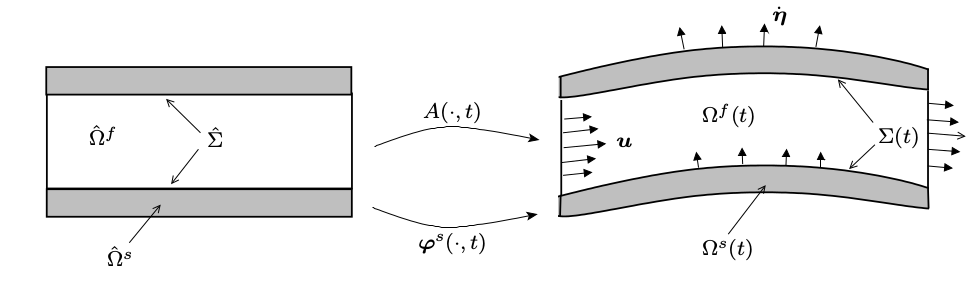
\includegraphics[width=14cm]{tools/MobileMesh.png}\end{center}
\texttt{\footnotesize{}extract from Donea J., Huerta A., Ponthot J. Ph. and Rodriguez-Ferran A., Encyclopedia of Computational Mechanic,
American Cancer Society, Arbitrary Lagrangian-Eulerian Methods, 2004}

\newpage
\chapter{Single-phase flow around a vibrating cylindrical tube}
\markboth{Single-phase flow around a vibrating cylindrical tube}{}
\def\orig{..}
% This file was generated automaticaly with the genererCources.py script
\documentclass[10pt,twoside,a4paper]{article}
\usepackage[ascii]{}
\usepackage{longtable}
\usepackage[utf8]{inputenc}
% \usepackage[french]{babel}
\usepackage{amsmath,amssymb,amsfonts,textcomp}
\usepackage{color}
% \usepackage{calc}
% \usepackage{hyperref}
% \hypersetup{colorlinks=true, linkcolor=blue, filecolor=blue, pagecolor=blue, urlcolor=blue}
\usepackage{graphicx}
\usepackage{fancyhdr}
% \usepackage[pdfpagemode=FullScreen,bookmarksopen=true,bookmarks=true]{hyperref}
\usepackage[bookmarksopen=true,bookmarks=true]{hyperref}

% \usepackage{verbatim}
%\usepackage{moreverb}
\usepackage{listings}

\setlength\hoffset{0cm}
\setlength\voffset{0cm}
\setlength\oddsidemargin{0cm}
\setlength\evensidemargin{0cm}
\setlength\topmargin{0cm}
\setlength\headheight{1cm}
\setlength\headsep{0.2cm}
\setlength\marginparsep{0cm}
\setlength\marginparwidth{0cm}
\setlength\footskip{2cm}
\setlength\textwidth{16cm}
\setlength{\parindent}{0pt}

% Style page
\renewcommand{\sectionmark}[1]{\markboth{#1}{#1}}
\pagestyle{fancy}
\lhead{\leftmark\\\rightmark}
\chead{}
\rhead{}
%\lfoot{\textit{Genere automatiquement avec genererCourbe.py, v0.1.}}
\lfoot{\textit{ Validation du fonctionnement du forcage spectral en presence de bulles.}}
\cfoot{}
\rfoot{\thepage}
\renewcommand{\headrulewidth}{0.4pt}
\renewcommand{\footrulewidth}{0.4pt}

\title{Validation du fonctionnement du forcage spectral en presence de bulles.}
\author{Gabriel Ramirez}
\date{02/09/2021}

\makeindex

% Debut document
\begin{document}
{\huge\centering Validation du fonctionnement du forcage spectral en presence de bulles. \par}

\section{Introduction}

Validation made by : Gabriel Ramirez.\\Report generated  02/09/2021.
\par\subsection{Description}

\par\subsection{Parameters TRUST }
\begin{itemize}
\item Version TRUST : 1.8.2
\end{itemize}
\par\subsection{Test cases}
\begin{itemize}
\item ADV\_X00/RUN00/spec\_bulles\_point2.data : \textit{}
\item NO\_ADV\_X00/RUN00/spec\_bulles\_point2.data : \textit{}
\item ADV\_0X0/RUN00/spec\_bulles\_point2.data : \textit{}
\item NO\_ADV\_0X0/RUN00/spec\_bulles\_point2.data : \textit{}
\item ADV\_010/RUN00/spec\_bulles\_point2.data : \textit{}
\item NO\_ADV\_010/RUN00/spec\_bulles\_point2.data : \textit{}
\item ADV\_001/RUN00/spec\_bulles\_point2.data : \textit{}
\item NO\_ADV\_001/RUN00/spec\_bulles\_point2.data : \textit{}
\item ADV\_101/RUN00/spec\_bulles\_point2.data : \textit{}
\item NO\_ADV\_101/RUN00/spec\_bulles\_point2.data : \textit{}
\end{itemize}

% Debut Chapitre
\section{Purpose}
Valider l'advection du champ de force. 

% Debut Chapitre
\section{Description du probl\`{e}me}
Le texte n'est pas a jour du tout. La suite de g\'{e}nr\'{e}rateur al\'{e}atoires se trouve dans .../OUT/random...out.
On impose un champ de force dans le domaine. Le champs de force est donn\'{e} par les \'{e}quations suivantes : 
 $F_{ph} = \mathcal{TF}(b(k,t_{i+1}) - \frac{k(k \cdot b(k, t_{i+1}))}{k \cdot k})$ 
$ b(k,t_{i+1}) = b(k,t_i)(1-\frac{\Delta t}{T_L}) + e_i(k,t) (2\sigma^2 \frac{\Delta t}{T_L})^{1/2}$
Le domaine est un cube de c\^{o}t\'{e} 01, allant de -0.005 a  0.005.
Chaque face est p\'{e}riodique
La viscosit\'{e} cin\'{e}matique est fix\'{e}e \`{a} 3.0128062836164946e-07 . La masse volumique \`{a} 1171.3. Il n'y a pas de phase gazeuse.


% Debut Chapitre
\section{Description du cas}
Le domaine est discr\'{e}tis\'{e} en $128^3$ \'{e}l\'{e}ments tous de m\^{e}me taille.

 On dispose quatre segments de relev\'{e} align\'{e}s selon X, quatre segments selon Y et 4 segments selon Z. 

% Debut Chapitre
\section{R\'{e}sultats}
On montre ici la visualitation des champs de la force spectrale ajout\'{e}e,
 obtenus avec l'outil de visualisation visit .


Force spectrale, avec reprises
 obtenus avec l'outil de visualisation visit .


Forces spectrales, obtenues d'une traite
 obtenus avec l'outil de visualisation visit .


Les marques correspondent aux premiers relev\'{e}s tels que l'autocorr\'{e}lation soit nulle ou n\'{e}gative.
     


% Debut Chapitre
\section{Conclusion}
En conclusion, on n'observe pas d'abh\'{e}rrance

% Debut Chapitre
\section{Computer performance}


% Debut tableau




% Fin du document
\end{document}

\newpage
\chapter{Hydrodynamic interaction of two cylinders subjected to small oscillations}
\markboth{Hydrodynamic interaction of two cylinders subjected to small oscillations}{}
\def\orig{..}
% This file was generated automaticaly with the genererCources.py script
\documentclass[10pt,twoside,a4paper]{article}
\usepackage[ascii]{}
\usepackage{longtable}
\usepackage[utf8]{inputenc}
% \usepackage[french]{babel}
\usepackage{amsmath,amssymb,amsfonts,textcomp}
\usepackage{color}
% \usepackage{calc}
% \usepackage{hyperref}
% \hypersetup{colorlinks=true, linkcolor=blue, filecolor=blue, pagecolor=blue, urlcolor=blue}
\usepackage{graphicx}
\usepackage{fancyhdr}
% \usepackage[pdfpagemode=FullScreen,bookmarksopen=true,bookmarks=true]{hyperref}
\usepackage[bookmarksopen=true,bookmarks=true]{hyperref}

% \usepackage{verbatim}
%\usepackage{moreverb}
\usepackage{listings}

\setlength\hoffset{0cm}
\setlength\voffset{0cm}
\setlength\oddsidemargin{0cm}
\setlength\evensidemargin{0cm}
\setlength\topmargin{0cm}
\setlength\headheight{1cm}
\setlength\headsep{0.2cm}
\setlength\marginparsep{0cm}
\setlength\marginparwidth{0cm}
\setlength\footskip{2cm}
\setlength\textwidth{16cm}
\setlength{\parindent}{0pt}

% Style page
\renewcommand{\sectionmark}[1]{\markboth{#1}{#1}}
\pagestyle{fancy}
\lhead{\leftmark\\\rightmark}
\chead{}
\rhead{}
%\lfoot{\textit{Genere automatiquement avec genererCourbe.py, v0.1.}}
\lfoot{\textit{ Validation du fonctionnement du forcage spectral en presence de bulles.}}
\cfoot{}
\rfoot{\thepage}
\renewcommand{\headrulewidth}{0.4pt}
\renewcommand{\footrulewidth}{0.4pt}

\title{Validation du fonctionnement du forcage spectral en presence de bulles.}
\author{Gabriel Ramirez}
\date{02/09/2021}

\makeindex

% Debut document
\begin{document}
{\huge\centering Validation du fonctionnement du forcage spectral en presence de bulles. \par}

\section{Introduction}

Validation made by : Gabriel Ramirez.\\Report generated  02/09/2021.
\par\subsection{Description}

\par\subsection{Parameters TRUST }
\begin{itemize}
\item Version TRUST : 1.8.2
\end{itemize}
\par\subsection{Test cases}
\begin{itemize}
\item ADV\_X00/RUN00/spec\_bulles\_point2.data : \textit{}
\item NO\_ADV\_X00/RUN00/spec\_bulles\_point2.data : \textit{}
\item ADV\_0X0/RUN00/spec\_bulles\_point2.data : \textit{}
\item NO\_ADV\_0X0/RUN00/spec\_bulles\_point2.data : \textit{}
\item ADV\_010/RUN00/spec\_bulles\_point2.data : \textit{}
\item NO\_ADV\_010/RUN00/spec\_bulles\_point2.data : \textit{}
\item ADV\_001/RUN00/spec\_bulles\_point2.data : \textit{}
\item NO\_ADV\_001/RUN00/spec\_bulles\_point2.data : \textit{}
\item ADV\_101/RUN00/spec\_bulles\_point2.data : \textit{}
\item NO\_ADV\_101/RUN00/spec\_bulles\_point2.data : \textit{}
\end{itemize}

% Debut Chapitre
\section{Purpose}
Valider l'advection du champ de force. 

% Debut Chapitre
\section{Description du probl\`{e}me}
Le texte n'est pas a jour du tout. La suite de g\'{e}nr\'{e}rateur al\'{e}atoires se trouve dans .../OUT/random...out.
On impose un champ de force dans le domaine. Le champs de force est donn\'{e} par les \'{e}quations suivantes : 
 $F_{ph} = \mathcal{TF}(b(k,t_{i+1}) - \frac{k(k \cdot b(k, t_{i+1}))}{k \cdot k})$ 
$ b(k,t_{i+1}) = b(k,t_i)(1-\frac{\Delta t}{T_L}) + e_i(k,t) (2\sigma^2 \frac{\Delta t}{T_L})^{1/2}$
Le domaine est un cube de c\^{o}t\'{e} 01, allant de -0.005 a  0.005.
Chaque face est p\'{e}riodique
La viscosit\'{e} cin\'{e}matique est fix\'{e}e \`{a} 3.0128062836164946e-07 . La masse volumique \`{a} 1171.3. Il n'y a pas de phase gazeuse.


% Debut Chapitre
\section{Description du cas}
Le domaine est discr\'{e}tis\'{e} en $128^3$ \'{e}l\'{e}ments tous de m\^{e}me taille.

 On dispose quatre segments de relev\'{e} align\'{e}s selon X, quatre segments selon Y et 4 segments selon Z. 

% Debut Chapitre
\section{R\'{e}sultats}
On montre ici la visualitation des champs de la force spectrale ajout\'{e}e,
 obtenus avec l'outil de visualisation visit .


Force spectrale, avec reprises
 obtenus avec l'outil de visualisation visit .


Forces spectrales, obtenues d'une traite
 obtenus avec l'outil de visualisation visit .


Les marques correspondent aux premiers relev\'{e}s tels que l'autocorr\'{e}lation soit nulle ou n\'{e}gative.
     


% Debut Chapitre
\section{Conclusion}
En conclusion, on n'observe pas d'abh\'{e}rrance

% Debut Chapitre
\section{Computer performance}


% Debut tableau




% Fin du document
\end{document}

\newpage
\chapter{Vibrations of a cylinder in a square tube bundle immersed in a viscous fluid}
\markboth{Vibrations of a cylinder in a square tube bundle immersed in a viscous fluid}{}
\def\orig{..}
% This file was generated automaticaly with the genererCources.py script
\documentclass[10pt,twoside,a4paper]{article}
\usepackage[ascii]{}
\usepackage{longtable}
\usepackage[utf8]{inputenc}
% \usepackage[french]{babel}
\usepackage{amsmath,amssymb,amsfonts,textcomp}
\usepackage{color}
% \usepackage{calc}
% \usepackage{hyperref}
% \hypersetup{colorlinks=true, linkcolor=blue, filecolor=blue, pagecolor=blue, urlcolor=blue}
\usepackage{graphicx}
\usepackage{fancyhdr}
% \usepackage[pdfpagemode=FullScreen,bookmarksopen=true,bookmarks=true]{hyperref}
\usepackage[bookmarksopen=true,bookmarks=true]{hyperref}

% \usepackage{verbatim}
%\usepackage{moreverb}
\usepackage{listings}

\setlength\hoffset{0cm}
\setlength\voffset{0cm}
\setlength\oddsidemargin{0cm}
\setlength\evensidemargin{0cm}
\setlength\topmargin{0cm}
\setlength\headheight{1cm}
\setlength\headsep{0.2cm}
\setlength\marginparsep{0cm}
\setlength\marginparwidth{0cm}
\setlength\footskip{2cm}
\setlength\textwidth{16cm}
\setlength{\parindent}{0pt}

% Style page
\renewcommand{\sectionmark}[1]{\markboth{#1}{#1}}
\pagestyle{fancy}
\lhead{\leftmark\\\rightmark}
\chead{}
\rhead{}
%\lfoot{\textit{Genere automatiquement avec genererCourbe.py, v0.1.}}
\lfoot{\textit{ Validation du fonctionnement du forcage spectral en presence de bulles.}}
\cfoot{}
\rfoot{\thepage}
\renewcommand{\headrulewidth}{0.4pt}
\renewcommand{\footrulewidth}{0.4pt}

\title{Validation du fonctionnement du forcage spectral en presence de bulles.}
\author{Gabriel Ramirez}
\date{02/09/2021}

\makeindex

% Debut document
\begin{document}
{\huge\centering Validation du fonctionnement du forcage spectral en presence de bulles. \par}

\section{Introduction}

Validation made by : Gabriel Ramirez.\\Report generated  02/09/2021.
\par\subsection{Description}

\par\subsection{Parameters TRUST }
\begin{itemize}
\item Version TRUST : 1.8.2
\end{itemize}
\par\subsection{Test cases}
\begin{itemize}
\item ADV\_X00/RUN00/spec\_bulles\_point2.data : \textit{}
\item NO\_ADV\_X00/RUN00/spec\_bulles\_point2.data : \textit{}
\item ADV\_0X0/RUN00/spec\_bulles\_point2.data : \textit{}
\item NO\_ADV\_0X0/RUN00/spec\_bulles\_point2.data : \textit{}
\item ADV\_010/RUN00/spec\_bulles\_point2.data : \textit{}
\item NO\_ADV\_010/RUN00/spec\_bulles\_point2.data : \textit{}
\item ADV\_001/RUN00/spec\_bulles\_point2.data : \textit{}
\item NO\_ADV\_001/RUN00/spec\_bulles\_point2.data : \textit{}
\item ADV\_101/RUN00/spec\_bulles\_point2.data : \textit{}
\item NO\_ADV\_101/RUN00/spec\_bulles\_point2.data : \textit{}
\end{itemize}

% Debut Chapitre
\section{Purpose}
Valider l'advection du champ de force. 

% Debut Chapitre
\section{Description du probl\`{e}me}
Le texte n'est pas a jour du tout. La suite de g\'{e}nr\'{e}rateur al\'{e}atoires se trouve dans .../OUT/random...out.
On impose un champ de force dans le domaine. Le champs de force est donn\'{e} par les \'{e}quations suivantes : 
 $F_{ph} = \mathcal{TF}(b(k,t_{i+1}) - \frac{k(k \cdot b(k, t_{i+1}))}{k \cdot k})$ 
$ b(k,t_{i+1}) = b(k,t_i)(1-\frac{\Delta t}{T_L}) + e_i(k,t) (2\sigma^2 \frac{\Delta t}{T_L})^{1/2}$
Le domaine est un cube de c\^{o}t\'{e} 01, allant de -0.005 a  0.005.
Chaque face est p\'{e}riodique
La viscosit\'{e} cin\'{e}matique est fix\'{e}e \`{a} 3.0128062836164946e-07 . La masse volumique \`{a} 1171.3. Il n'y a pas de phase gazeuse.


% Debut Chapitre
\section{Description du cas}
Le domaine est discr\'{e}tis\'{e} en $128^3$ \'{e}l\'{e}ments tous de m\^{e}me taille.

 On dispose quatre segments de relev\'{e} align\'{e}s selon X, quatre segments selon Y et 4 segments selon Z. 

% Debut Chapitre
\section{R\'{e}sultats}
On montre ici la visualitation des champs de la force spectrale ajout\'{e}e,
 obtenus avec l'outil de visualisation visit .


Force spectrale, avec reprises
 obtenus avec l'outil de visualisation visit .


Forces spectrales, obtenues d'une traite
 obtenus avec l'outil de visualisation visit .


Les marques correspondent aux premiers relev\'{e}s tels que l'autocorr\'{e}lation soit nulle ou n\'{e}gative.
     


% Debut Chapitre
\section{Conclusion}
En conclusion, on n'observe pas d'abh\'{e}rrance

% Debut Chapitre
\section{Computer performance}


% Debut tableau




% Fin du document
\end{document}

%%%%%%%%%%%%%%%%%%%%%%%%%%%%%%%%%%%%%%%%%%%%%%%%%%%%%%%%%%%%%%%%%%%%%%%%%%%%%%%%%%%%%%
\part{Conclusion}
\markboth{}{CONCLUSION}
\chead{
\tikz[remember picture,overlay] {%
    \fill [White,fill opacity=.2]
    ([yshift=0pt]current page header area.south west -| current page.north west)
    rectangle
    (current page.north east)
    ;
    \fill [White,fill opacity=.2]
    ([yshift=-45pt]current page.south west)
    rectangle
    (current page footer area.north east -| current page.north east)
    ;
  }
}
\normalsize \normalfont
\lettrine[lines=2,slope=0pt,nindent=4pt]{\textbf{T}}{his} document
is the first version of a \texttt{TrioCFD} validation report resulting
of an analysis and a sorting work that have been done on its database.
First, an important inventory job was carried out in order to sort
the test cases for targeting quickly the use of \texttt{TrioCFD}
in different CFD configurations. The inventory resulted in a single
table with plenty information (LibreOffice format), where the test
cases are classified into several subdomains of fluid flows. In this
document, some of them have been selected and detailed because 1)
they are well-known in the literature, 2) they present comparisons
with other academic or commercial CFD codes, 3) they present comparisons
with experimental data and 4) they cover an important and representative part of the
physics of the code. In this report, the test cases are representative
of five subdomains: ``Laminar flow'' (Part III), ``Thermal laminar
flow'' (Part IV), ``Turbulent flow'' (Part V), ``Thermal turbulent
flow'' (Part VI), ``Front Tracking'' (Part VII) and "Fluid/structure
interactions with ALE" (Part VIII). The first four
parts gather the test cases for single phase flows, coupled or not with
turbulence models and thermal effects. Part VII is dedicated
to two-phase flows with interface tracking and the last part (VIII) that
has been added since the last version of this report focuses on fluid/structure
interactions with Arbitrary Lagrangian-Eulerian Method (ALE). The corresponding datafiles
were run with the \texttt{1.8.2} version of \texttt{TrioCFD}
to check the achievement of computations. Meanwhile, an important
work was carried out to update a new \texttt{PRM} template in order
to standardize all validation sheets. For each one of them, let us
remind that the PDF file is generated by running a bash script (command
\texttt{Run\_fiche -not\_run}) which acts on a \texttt{PRM} file (previously, test cases must have
been run). A \texttt{PRM} file is a set of specific instructions for interfacing
the \LaTeX ~commands with the \texttt{TrioCFD} results post-processed
with \texttt{Gnuplot} or \texttt{Visit}. Its content can be freely
chosen by authors which has the consequence that the number and titles
of sections differ from one sheet to another one. The goal of the
new \texttt{PRM} template is to harmonize their contents for a more
homogeneous rendering of this report. The seven sections of the new
\texttt{PRM} template detail the main stages of CFD modeling and describe
the comparisons. All validation sheets in this report have been revised
and enhanced by taking into account this new \texttt{PRM} template.

\section*{Perspective}

Numerous other validation sheets already exist in the \texttt{TrioCFD}
database and the job must be pursued. Hence, this document does not
present an exhaustive list of what \texttt{TrioCFD} can do for CFD
applications. It can be viewed as a simple ``snapshot'' that will
be gradually improved and increased at each version release. The improvement
will be simplified by the methodology and the tools which have been
developed for \texttt{PRM} files. After checking and updating the
validations sheets, they will be added in the future versions of this
report. Among the available test cases, the sort will be pursued to
separate those currently ``in progress'' and the others that lack
quantitative comparisons. Multiple variations of the same test case
appear in the database (e.g. ``Poiseuille flow''). Some of them
are simply a 3D extension of the same test case, or an extension with
temperature equation or turbulence model. For instance, the laminar
test case of ``flow with a cylinder'' (Chapter III.3) exists in
turbulent version in two and three dimensions. Another example is
given by the test case named ``Backward facing step'' which appears
in four different versions: the first one is ``two-dimensional'',
the second one is ``implicit'', the third one is ``three-dimensional''
and the last one is ``heated in two dimensions''. More test cases
of turbulent flow are also available, such as ``Baglietto'' and
``Flow in curved pipe''. An effort will be done to extend the
number of CFD subdomains such as ``Quasi-compressible flow'', ``Flow
in porous media'' and ``fluid-structure interaction''. Finally
several tests are dedicated to the ``grid convergence'' or ``Miscellaneous
test'' of numerical options.

%%%%%%%%%%%%%%%%%%%%%%%%%%%%%%%%%%%%%%%%%%%%%%%%%%%%%%%%%%%%%%%%%%%%%%%%%%%%%%%%%%%%%%
\begin{landscape}
\section*{Annexe A: List of TrioCFD \texttt{PRM} files}

\rhead{Annexe A: List of TrioCFD \texttt{PRM} files}
\addcontentsline{toc}{part}{Annexe A: List of TrioCFD \texttt{PRM} files}
\begin{table}[H]
\begin{centering}
\begin{longtable}{lclccclc}
\hline
\textbf{PDF File name} & \textbf{Problem} & \textbf{Dis.} & \textbf{Dim.} & \textbf{Mesh} & \textbf{Nb jdds} & \textbf{Goal of the sheet} & \textbf{State} \\
\hline
\noalign{\vskip0.1cm}
\hline
\endhead
\hline
\endfoot
\rowcolor{LimeGreen} \multicolumn{8}{c}{\textbf{Laminar Flow}} \\
\hline
\rowcolor{LimeGreen!10}Channel\_lam\_pressure\_drop & Pb\_hydraulique & VDF & 3 & 160 hexa & 21 & Convection schemes - Periodic BC & old format \\ 
\rowcolor{LimeGreen!10} &  & VEF & & 1920 tetra &  & fluid : helium &  \\
\hline
\rowcolor{LimeGreen!10}Cir\_Cyl\_Re100 & Pb\_hydraulique & VEF & 2 & 9668 triang. & 2 & Explicit Euler with implicit & new format \\
\rowcolor{LimeGreen!10} &  &  &  &  &  & diffusion - literature comparison & report \\
\hline
\rowcolor{LimeGreen!10}ConvergenceTaylorGreen & Pb\_hydraulique & VEF & 2 & 4 $\Rightarrow$ 256 to & 20 & Convergence for different & old format \\
\rowcolor{LimeGreen!10} & & & & 16384 triang. & & meshes and convection scheme & \\
\hline
\rowcolor{LimeGreen!10}ConvergenceTaylorGreen & Pb\_hydraulique & VEF & 2 & 3 $\Rightarrow$ 256 to & 54 & Convergence for different & old format \\
\rowcolor{LimeGreen!10}WithDiffusion & & & & 4096 triang. & & meshes and time scheme & \\
\hline
\rowcolor{LimeGreen!10}DirectionalPressureLoss & Pb\_hydraulique & VEF & 3 & 3 $\Rightarrow$ 1152, 9216 & 6 & Validation of 64 bits & old format \\
\rowcolor{LimeGreen!10} & & & & and 73728 tetra & & integers possibility to configure &  \\
\hline
\rowcolor{LimeGreen!10}FVCA\_test\_EF\_stab & Pb\_hydraulique & VEF & 3 & 7 $\Rightarrow$ 27 to & 70 & Convergence orders of the & old format \\ 
\rowcolor{LimeGreen!10} &  &  &  & 1728 tetra & & EF\_stab convection schemes &  \\
\hline
\rowcolor{LimeGreen!10}FVCAB\_Cas\_2.2\_3D\_steady & Pb\_hydraulique & VEF & 3 & 7 $\Rightarrow$ 215 to 61052 tetra& 12 & 3D Taylor-Green vortex  & old format \\ 
\rowcolor{LimeGreen!10}\_Stokes\_Taylor\_Green\_vortex &  & VDF &  & 5 $\Rightarrow$ 8 to 32768 hexa &  & FVCAB experiments &  \\
\hline
\rowcolor{LimeGreen!10}Lid\_driven\_cavity & Pb\_hydraulique & VEF & 2 & 105724 triang. & 1 & \textbf{Implicit Euler steady scheme} & new format \\
\rowcolor{LimeGreen!10}& & & & & & comparison with litterature & report \\
\hline
\rowcolor{LimeGreen!10}Poiseuilleperio2D & Pb\_hydraulique & VEF & 2 & 6 $\Rightarrow$ 6, 24, 96 & 18 & Poiseuille comparisons: EF\_stab & old format \\
\rowcolor{LimeGreen!10} & & & & 384, 1536, 6144 triang. & & versus Amont schemes & \\
\hline
\rowcolor{LimeGreen!10}PoiseuillePerio2DVEF & Pb\_hydraulique & VEF & 3 & 2785 triang. & 2 & EF\_stab versus Amont schemes  & old format \\
\rowcolor{LimeGreen!10}\_prismes & & & & & & with an ICEM generated VEF mesh & \\
\hline
\rowcolor{LimeGreen!10}PoiseuillePerio2DVEF & Pb\_hydraulique & VEF & 2 & 8 $\Rightarrow$ 6 to  & 20 & EF\_stab versus Amont schemes & old format \\
\rowcolor{LimeGreen!10}\_fNcells & & & & 98304 triang. & & with different mesh sizes & \\
\hline
\rowcolor{LimeGreen!10}PoiseuillePerio2DVEF & Pb\_hydraulique & VEF & 2 & 2785 triang. & 3 & EF\_stab versus Amont schemes & old format \\
\rowcolor{LimeGreen!10}\_fNcells\_prismes & & & & & & with an ICEM generated VEF mesh &  \\
\hline
\end{longtable}
\end{centering}
\end{table}

\newpage

\begin{table}[H]
\begin{centering}
\begin{tabular}{lclccclc}
\hline
\textbf{PDF File name} & \textbf{Problem} & \textbf{Dis.} & \textbf{Dim.} & \textbf{Mesh} & \textbf{Nb jdds} & \textbf{Goal of the sheet} & \textbf{State} \\
\hline \noalign{\vskip0.1cm} \hline
\hline
\rowcolor{LimeGreen} \multicolumn{8}{c}{\textbf{Laminar Flow}} \\
\hline
\rowcolor{LimeGreen!10}PoiseuillePerio2DVEF & Pb\_hydraulique & VEF & 2 & 6 $\Rightarrow$ 6 to  & 20 & Convection schemes comparison & old format \\
\rowcolor{LimeGreen!10}\_fNcells\_trianfin & & VEF & & 24576 triang. & & mesh created using trianguler\_fin & \\
\hline
\rowcolor{LimeGreen!10}Poiseuille\_flow\_2D & Pb\_hydraulique & VDF & 2 & 200 rect. & 5 & Validation of the incompressible laminar & new format \\
\rowcolor{LimeGreen!10}\_VDF\_VEF & & VEF & & 400 triang. & & module with analytical solution & report \\
\hline
\rowcolor{LimeGreen!10}PoiseuilleInOutVDFVEF & Pb\_hydraulique & VDF & 2 & 600 rect. & 10 & Hydraulic with pressure drop & old format \\ 
\rowcolor{LimeGreen!10} & & VEF & & 1200 triang. & & & \\
\hline
\rowcolor{LimeGreen!10}PoiseuilleInOut2DVDFVEF & Pb\_hydraulique & VDF & 2 & 600 rect. & 10 & Hydraulic with pressure drop & old format \\ 
\rowcolor{LimeGreen!10}\_trianfin & & VEF & & 4800 triang. & & mesh created using trianguler\_fin & \\
\hline
\rowcolor{LimeGreen!10}PoiseuilleInOut2DVDFVEF & Pb\_hydraulique & VDF & 2 & 600 rect. & 10 & Hydraulic with pressure drop & old format \\ 
\rowcolor{LimeGreen!10}\_prismes & & VEF & & 3474 triang. & & ICEM generated VEF mesh &  \\
\hline
\rowcolor{LimeGreen!10}poiseuille\_3D & Pb\_hydraulique & VEF & 3 & 17360 tetra. & 5 & Hydraulic with pressure drop & old format \\ 
\rowcolor{LimeGreen!10} & & & & & & comparison of 2 convection schemes  & \\
\hline
\rowcolor{LimeGreen!10}PoiseuillePerio3DVDFVEF & Pb\_hydraulique & VDF & 3 & 160 hexa. & 28 & Validation of convection and time schemes & old format \\ 
\rowcolor{LimeGreen!10}\_fRe & & VEF & & 1920 tetra. & &  Tetraedrisation for VEF discretization & \\
\hline
\rowcolor{LimeGreen!10}PoiseuillePerio3DVDFVEF & Pb\_hydraulique & VDF & 3 & 160 hexa. & 28 & VEF mesh is created using tetraedriser& old format \\ 
\rowcolor{LimeGreen!10}\_fRe\_tetrafin & & VEF & & 15360 tetra & &  \_homogene\_fin - improved results &  \\
\hline
\rowcolor{LimeGreen!10}PoiseuillePerio3DVDFVEF & Pb\_hydraulique & VDF & 3 & 160 hexa. & 28 & Same as previous with VEF mesh & old format \\ 
\rowcolor{LimeGreen!10}\_fRe\_prismes & & VEF & & 29313 tetra. & & generated with ICEM &  \\
\hline
\rowcolor{LimeGreen!10}Poiseuille\_Pipe\_Velocity & Pb\_hydraulique & VEF & 3 & 126560 tetra & 4 & Validation of different convection schemes & old format \\ 
\rowcolor{LimeGreen!10} & & & & & & & \\
\hline
\rowcolor{LimeGreen!10}Diagonale\_Cube & \textbf{Pb\_hydraulique} & VEF & 3 & 192000 tetra. & 5 & Convection schemes recommandations for 3D  & old format \\ 
\rowcolor{LimeGreen!10} & \textbf{\_concentration} & & & & & scalar passive transport & \\
\hline
\rowcolor{LimeGreen!10} test\_div\_grad\_Prep1b & Pb\_hydraulique & VEF & 2 & 1324 tri & 5 & Laminar flow through a plane channel & old format \\
\rowcolor{LimeGreen!10} & & & & & & coding verification & \\
\hline
\rowcolor{LimeGreen!10}Mixing\_Bidim\_Axi & \textbf{Pb\_hydraulique} & VDF & 2 & 5 $\Rightarrow$ 5784 to & 5 & Comparison of the dispersion coefficient & old format \\ 
\rowcolor{LimeGreen!10} & \textbf{\_concentration} & & Axi & 1439232 rect. & & with experimental for different meshes & \\
\hline
\end{tabular}
\end{centering}
\end{table}

\newpage

\begin{table}[H]
\begin{centering}
\begin{tabular}{lclccclc}
\hline
\textbf{PDF File name} & \textbf{Problem} & \textbf{Dis.} & \textbf{Dim.} & \textbf{Mesh} & \textbf{Nb jdds} & \textbf{Goal of the sheet} & \textbf{State} \\
\hline
\noalign{\vskip0.1cm}
\hline
\hline
\rowcolor{LimeGreen} \multicolumn{8}{c}{\textbf{Laminar Flow}} \\
\hline
\rowcolor{LimeGreen!10}Turbulence\_synthetique & Pb\_hydraulique & VDF & 3 & 1024 to 65536 hexa & 15 & Generation of isotropic synthetic & new format \\ 
\rowcolor{LimeGreen!10}& & VEF & & 6144 to 16777216 hexa & 8 & fluctuations as inlet boundary condition &  \\
\hline
\rowcolor{LimeGreen!10}Vorticite\_et\_fonction & Pb\_hydraulique & VDF & 2 & 7 $\Rightarrow$ 16 to 65536 rect & 40 & Verification of vorticity and & old format \\ 
\rowcolor{LimeGreen!10}\_de\_Courant & \textbf{Pb\_conduction} & VEF & & 7 $\Rightarrow$ 16 to 65536 quad & & Stream function in a square cavity &  \\ 
\rowcolor{LimeGreen!10} &  & VEF & & 6 $\Rightarrow$ 40 to 104420 tri & & & \\
\hline
\rowcolor{LimeGreen!10}2D\_VEF\_Cylindre & Pb\_hydraulique & VEF & 2 & 999 tri & 1 & \textbf{Implicit\_Euler\_steady\_scheme} & old format \\
\rowcolor{LimeGreen!10}\_steady & & & & & & \textbf{Numerical Test} & \\
\hline
\rowcolor{LimeGreen!10}Navier\_Stokes\_2d & Pb\_hydraulique & VEF & 2 & 104420 tri. & 8 & \textbf{Implicit\_Euler\_steady\_scheme} & old format \\
\rowcolor{LimeGreen!10}\_steady & & & & & & \textbf{Numerical}: comparison with analytical & \\
\hline
\rowcolor{LimeGreen!10}Navier\_Stokes\_3d & Pb\_hydraulique & VEF & 3 & 61052 tetra & 3 & \textbf{Implicit\_Euler\_steady\_scheme} & old format \\ 
\rowcolor{LimeGreen!10}\_steady & & & & & & \textbf{Numerical}: comparison with analytical & \\
\hline
\rowcolor{LimeGreen!10}NoFlow & Pb\_hydraulique & VEF & 2 & 3 $\Rightarrow$ 242, 1054 & 24 & \textbf{Validation of the $P_0-RT$ scheme} & old format \\ 
\rowcolor{LimeGreen!10} & & \textbf{P0 RT} & & \& 4262 tri. & & in case of a $\vec{u}=0$ & \\
\hline
\rowcolor{LimeGreen!10}StatVortex2D & Pb\_hydraulique & VEF & 2 & 3 $\Rightarrow$ 242, 1054 & 24 & \textbf{Validation of the $P_0-RT$ scheme} & old format \\ 
\rowcolor{LimeGreen!10} & & \textbf{P0 RT} & & \& 4262 tri. & & for a steady state 2D vortex &  \\
\hline
\rowcolor{LimeGreen!10}StatVortex & Pb\_hydraulique & VEF & 3 & 4 $\Rightarrow$ 215 & 40 & \textbf{Validation of the $P_0-RT$ scheme} & old format \\ 
\rowcolor{LimeGreen!10} & & \textbf{P0 RT} & & to 7711 tetra & & for a steady state 3D vortex & \\
\hline
\rowcolor{LimeGreen!10}RotFlow & Pb\_hydraulique & VEF & 2 & 3 $\Rightarrow$ 242, 1054 & 24 & \textbf{Validation of the $P_0-RT$ scheme} & old format \\ 
\rowcolor{LimeGreen!10} & & \textbf{P0 RT} & & \& 4262 tri. & & for a rotational velocity & \\
\hline
\end{tabular}
\end{centering}
\end{table}


\newpage

\begin{table}[H]
\begin{centering}
\begin{tabular}{lclccclc}
\hline
\textbf{PDF File name} & \textbf{Problem} & \textbf{Dis.} & \textbf{Dim.} & \textbf{Mesh} & \textbf{Nb jdds} & \textbf{Goal of the sheet} & \textbf{State} \\
\hline \noalign{\vskip0.1cm}
\hline
\hline
\rowcolor{ForestGreen} \multicolumn{8}{c}{\textbf{Thermal Laminar Flow}} \\
\hline
\rowcolor{ForestGreen!10}Convection\_Rotating & Pb\_thermohydraulique & VEF & 2 & 6130 tri & 28 & Laminar advection of temperature & old format \\ 
\rowcolor{ForestGreen!10}\_Table & & & & & & fields on a circular rotating table & \\
\hline
\rowcolor{ForestGreen!10}Convection\_Vahl\_Davis & Pb\_thermohydraulique & VDF & 2 & 4761 rect & 10 & Validation of the coupling & new format \\ 
\rowcolor{ForestGreen!10} & & VEF & & 1444 \& 6084 tri & & between flow and thermics & \\
\rowcolor{ForestGreen!10} & & & & & & in laminar condition & \\
\hline
\rowcolor{ForestGreen!10}Oscillating\_Flow & Pb\_thermohydraulique & VDF & 2 & 2500 rect & 5 & Natural convection inside a  & new format \\ 
\rowcolor{ForestGreen!10} & & VEF & & 5040 tri & & rectangular heated cavity & report \\
\hline
\rowcolor{ForestGreen!10}Pb\_couple\_2D & Pb\_thermohydraulique & VDF & 2 & 36 rect & 2 & Laminar heat exchange through a & old format \\
\rowcolor{ForestGreen!10} & \textbf{Pb\_conduction} & VEF & & 64 tri & & plane channel with wall conduction & \\
\hline
\rowcolor{ForestGreen!10}PorousWithPLoss & Pb\_thermohydraulique & VEF & 2 & 84 tri & 4 & Laminar flow in a channel with & old format \\ 
\rowcolor{ForestGreen!10} \_VEF & & VEF & 3 & 486 tetra & & porous media and pressure loss & \\
\hline
\rowcolor{ForestGreen!10}VAHL\_DAVIS\_impl & Pb\_thermohydraulique & VDF & 2 & 10000 rect & 22 & Comparison of velocity and & old format \\ 
\rowcolor{ForestGreen!10} & & VEF & & 6400 tri & & temperature profiles & \\
\rowcolor{ForestGreen!10} & & & & & & using explicit or implicit algo & \\
\hline
\rowcolor{ForestGreen!10} & Pb\_thermohydraulique & VDF & 2 & 39402 rect & 2 & Vertical flat heated plate & \\ 
\rowcolor{ForestGreen!10}therm\_stratif & & VDF & 3 & 86246 hexa & 2 & immersed in pool of water & old format \\
\rowcolor{ForestGreen!10}\_water\_tank & & VEF & 2 & 18816 tri & 2 & open to atmosphere & \\
\rowcolor{ForestGreen!10} & & VEF & 3 & 86400 tetra & 2 & & \\
\hline
\rowcolor{ForestGreen!10}ThHyd\_3D\_VEF & Pb\_thermohydraulique & VEF & 3 & 1270 tetra & 1 & \textbf{Implicit\_Euler} & old format \\
\rowcolor{ForestGreen!10} \_steady & & & & & & \textbf{\_steady\_scheme} & \\
\rowcolor{ForestGreen!10} & & & & & & \textbf{Numerical Test} & \\
\hline
\rowcolor{ForestGreen!10}& & VDF & 2 & 20+25 and 100 rect & & Coupling between radiation, & \\
\rowcolor{ForestGreen!10} & Pb\_Thermohydraulique & VEF & 2 & 80+40 and 1600 tri & & Conduction and natural convection  & \\ 
\rowcolor{ForestGreen!10}Radiation & \textbf{Pb\_conduction} & VDF & 3 & 100+125 and 125 hexa & 10 & inside a 2D or 3D channel & old format \\
\rowcolor{ForestGreen!10} & \textbf{Pb\_Couple\_Rayonnement} & VEF & 3 & 1958+1220 to 5884 tetra & & \textbf{Radiation in} & \\ 
\rowcolor{ForestGreen!10} & & VDF & Axi & 100 rect & & \textbf{transparent medium} & \\ 
\rowcolor{ForestGreen!10} & & & & & & \textbf{Pb\_Couple\_Rayonnement} & \\
\hline
\end{tabular}
\end{centering}
\end{table}

\newpage

\begin{table}[H]
\begin{centering}
\begin{tabular}{lclccclc}
\hline
\textbf{PDF File name} & \textbf{Problem} & \textbf{Dis.} & \textbf{Dim.} & \textbf{Mesh} & \textbf{Nb jdds} & \textbf{Goal of the sheet} & \textbf{State} \\
\hline \noalign{\vskip0.1cm} \hline
\hline
\rowcolor{SkyBlue} \multicolumn{8}{c}{\textbf{Turbulent Flow}} \\
\hline
\rowcolor{SkyBlue!10}Backward\_Facing & Pb\_hydraulique\_Turbulent & VEF & 2 & 2944 tri & 11 & Turbulent channel air flow with back- & old format \\ 
\rowcolor{SkyBlue!10}\_Step\_impl & & & & & & ward step - $\kappa-\epsilon$ + loi\_standard\_hydr &  \\
\hline
\rowcolor{SkyBlue!10}Backward\_Facing & Pb\_hydraulique\_Turbulent & VDF & 3 & 28620 rect & 2 & Turbulent channel air flow with back- & old format \\ 
\rowcolor{SkyBlue!10}\_Step\_3D & & VEF & & 366230 tri & & ward step - $\kappa-\epsilon$ + loi\_standard\_hydr & \\
\hline
\rowcolor{SkyBlue!10}Backward\_Facing & Pb\_hydraulique\_Turbulent & VDF & 2 & 3228 rect & 6 & $\kappa-\epsilon$ + loi\_standard\_hydr  & old format \\ 
\rowcolor{SkyBlue!10}\_Step & & VEF & & 2944 tri & & or loi\_expert\_hydr & \\
\hline
\rowcolor{SkyBlue!10}ChannelPerio2D & Pb\_hydraulique\_Turbulent & VEF & 3 & 4 $\Rightarrow$ 80 $\to$ 640 tri & 8 & Longueur\_Melange +  & old format \\ 
\rowcolor{SkyBlue!10}VEF\_fNy & & & & & & loi\_standard\_hydr &  \\
\hline
\rowcolor{SkyBlue!10}Turbulent\_perio & Pb\_hydraulique\_Turbulent & VEF & 2 & 6 $\Rightarrow$ 6 $\to$ 6144 tri & 24 & Comparison of convection schemes -  & old format \\
\rowcolor{SkyBlue!10} \_2D\_channel & & & & & & Longueur\_Melange+loi\_standard\_hydr & \\
\hline
\rowcolor{SkyBlue!10}ChannelML3DVDF & Pb\_hydraulique\_Turbulent & VDF & 3 & 3 $\Rightarrow$ 684 to  & 19 & Longueur\_Melange & old format \\
\rowcolor{SkyBlue!10}\_fNydxdz & & & & 10516 hexa & & + loi\_standard\_hydr & \\
\hline
\rowcolor{SkyBlue!10}ChannelML3DVEF & Pb\_hydraulique\_Turbulent & VEF & 3 & 960 \& 3840 tetra & 24 & Longueur\_Melange + loi\_expert\_hydr & old format \\ 
\rowcolor{SkyBlue!10}\_fNydxdz & & & & 2348 $\to$ 47405 tetra & & & \\
\hline
\rowcolor{SkyBlue!10}ChannelMLPerio3D & Pb\_hydraulique\_Turbulent & VEF & 3 & 480 tetra & 12 & Turbulent helium flow through & old format \\ 
\rowcolor{SkyBlue!10}VEF\_fRe & & & & & & a periodic plane channel &  \\
\hline
\rowcolor{SkyBlue!10}ChannelMLPerio3D & Pb\_hydraulique\_Turbulent & VEF & 3 & 3840 tetra & 12 & Same than previous with mesh & old format \\ 
\rowcolor{SkyBlue!10}VEF\_fRe\_tetrafin & & & & & & refinement - better results for high Re & \\
\hline
\end{tabular}
\end{centering}
\end{table}

\newpage

\begin{table}[H]
\begin{centering}
\begin{tabular}{lclccclc}
\hline
\textbf{PDF File name} & \textbf{Problem} & \textbf{Dis.} & \textbf{Dim.} & \textbf{Mesh} & \textbf{Nb jdds} & \textbf{Goal of the sheet} & \textbf{State} \\
\hline \noalign{\vskip0.1cm} \hline
\hline
\rowcolor{SkyBlue} \multicolumn{8}{c}{\textbf{Turbulent Flow}} \\
\hline
\rowcolor{SkyBlue!10}KEps\_Meshing & Pb\_hydraulique\_Turbulent & VEF & 3 & 960 \& 3840 tetra & 23 & Meshing tests for 3D VEF-plane & old format \\ 
\rowcolor{SkyBlue!10}\_VEF & & & & 11735 $\to$ 16551 tetra & & channel with $\kappa-\epsilon$ model & \\
\hline
\rowcolor{SkyBlue!10}ChannelkepsPerio & Pb\_hydraulique\_Turbulent & VEF & 3 & 480 tetra & 12 & Pressure drop in a 3D periodic & old format \\ 
\rowcolor{SkyBlue!10}3DVEF\_fRe & & & & & & turbulent flow  in a plane channel & \\
\hline
\rowcolor{SkyBlue!10}ChannelkepsPerio & Pb\_hydraulique\_Turbulent & VEF & 3 & 3840 tetra & 12 & Same than previous with mesh & old format \\ 
\rowcolor{SkyBlue!10}3DVEF\_fRe\_tetrafin & & & & & & refinement - $\kappa-\epsilon$ + loi\_expert\_hydr & \\
\hline
\rowcolor{SkyBlue!10}Channelkeps & Pb\_hydraulique\_Turbulent & VDF & 3 & 3 $\Rightarrow$ 684, 2332 & 18 & Meshing tests for 3D VDF plane & old format \\ 
\rowcolor{SkyBlue!10}3DVDF\_fNydxdz & & & & \& 10516 hexa & & channel with $\kappa-\epsilon$ model &  \\
\hline
\rowcolor{SkyBlue!10}Channelkeps & Pb\_hydraulique\_Turbulent & VEF & 3 & 960 \& 3840 tetra & 24 & Meshing tests for 3D VEF plane & old format \\ 
\rowcolor{SkyBlue!10}3DVEF\_fNydxdz & & & & 5 $\Rightarrow$ 2348 $\to$ 47405 & & channel with $\kappa-\epsilon$ model & \\
\hline
\rowcolor{SkyBlue!10}ChannelKEps\_CLboite & Pb\_hydraulique\_Turbulent & VEF & 3 & 13552 tetra & 1 & Periodic box on a turbulent flow in a & old format \\ 
\rowcolor{SkyBlue!10}Perio\_entree & & & & & & plane channel with $\kappa-\epsilon$ model & \\
\hline
\rowcolor{SkyBlue!10}k\_eps\_vef & Pb\_hydraulique\_Turbulent & VEF & 3 & 1152 tetra & 1 & Verification of friction velocity in a  & old format \\ 
\rowcolor{SkyBlue!10}\_perio & & & & & & periodic plane channel with $\kappa-\epsilon$ model & \\
\hline
\rowcolor{SkyBlue!10}Canal\_plan\_VDF\_VEF & & VDF & 2 & 276 rect & 2 & Comparaison of the coupled and  & \\ 
\rowcolor{SkyBlue!10}\_k\_eps\_standard & Pb\_hydraulique\_Turbulent & VEF & 2 & 172 tri & 2 & decoupled methods for solving  & new format \\
\rowcolor{SkyBlue!10}\_bicephale & & VDF & 3 & 828 hexa & 2 & the $\kappa-\epsilon$ transport equations & \\ 
\rowcolor{SkyBlue!10} & & VEF & 3 & 1982 tetra & 2 & k\_epsilon\_bicephale & \\ 
\hline
\end{tabular}
\end{centering}
\end{table}

\newpage

\begin{table}[H]
\begin{centering}
\begin{tabular}{lclccclc}
\hline
\textbf{PDF File name} & \textbf{Problem} & \textbf{Dis.} & \textbf{Dim.} & \textbf{Mesh} & \textbf{Nb jdds} & \textbf{Goal of the sheet} & \textbf{State} \\
\hline \noalign{\vskip0.1cm}
\hline
\hline
\rowcolor{SkyBlue} \multicolumn{8}{c}{\textbf{Turbulent Flow}} \\
\hline
\rowcolor{SkyBlue!10}expansion\_2D\_axi\_3D & Pb\_hydraulique\_Turbulent & VDF & Axi & 5577 rect & 5 & Expanding turbulent flow with & old format \\ 
\rowcolor{SkyBlue!10}\_VEF\_circular & & VEF & 3 & 65923 tetra & 5 & various inlet velocities & \\
\hline
\rowcolor{SkyBlue!10}expansion\_3D & Pb\_hydraulique\_Turbulent & VDF & 3 & 48400 hexa & 5 & Same than previous in 3D  & old format \\
\rowcolor{SkyBlue!10}\_VDF\_VEF & & VEF & & 51840 tetra & 5 & with VDF and VEF mesh & \\
\hline
\rowcolor{SkyBlue!10}Mixing\_length & Pb\_hydraulique\_Turbulent & VEF & 2 & 7 $\Rightarrow$ 80 to  & 14 & Mixing length in 2D and 3D & new format \\
\rowcolor{SkyBlue!10}\_VEF\_WF & & VEF & 3 & 7680 tetra & & VEF-plane channel & report \\
\hline
\rowcolor{SkyBlue!10}OBI\_diffuser\_VEF & Pb\_hydraulique\_Turbulent & VEF & 2 & 36644 tetra & 2 & Turbulent flow in a 2D diffuser & new format \\ 
\rowcolor{SkyBlue!10}\_k\_eps & & & & & & with the $\kappa-\epsilon$ model & report \\
\hline
\rowcolor{SkyBlue!10}Tube\_turb\_perio & Pb\_hydraulique\_Turbulent & VEF & 3 & 78576 tetra & 1 & Fully developed turbulent flow & old format \\ 
\rowcolor{SkyBlue!10}\_EF\_stab & & & & & & in circular tube & \\
\hline
\rowcolor{SkyBlue!10}Tube\_turb\_perio & Pb\_hydraulique\_Turbulent & VEF & 3 & 78576 tetra & 1 & Same than previous with muscl scheme & old format \\ 
\rowcolor{SkyBlue!10}\_muscl & & & & & & better prediction of  turbulent viscosity  & \\
\hline
\rowcolor{SkyBlue!10}EsthairNoWire & Pb\_hydraulique\_Turbulent & VEF & 3 & 3 $\Rightarrow$ 3114 to  & 5 & Esthair calculations of a 19 rods & old format \\ 
\rowcolor{SkyBlue!10} & & & & 11829 tetra & & sub-assembly without space wire & \\
\hline
\rowcolor{SkyBlue!10}ContractionTurbFlow & Pb\_hydraulique\_Turbulent & VEF & 3 & 684 \& 1260 & 6 & Pressure loss through a  & old format \\ 
\rowcolor{SkyBlue!10}\_3D\_VEF & & & & 29011 \& 107842 & & sudden contraction & \\
\hline
\rowcolor{SkyBlue!10}Cube\_Atmo & Pb\_hydraulique\_Turbulent & VEF & 3 & 2 $\Rightarrow$ 42964 and & 4 & Atmospheric flow around & old format \\ 
\rowcolor{SkyBlue!10} & & & & 55183 hexa & & a cube &  \\
\hline
\rowcolor{SkyBlue!10}Couche\_Limite & Pb\_hydraulique\_Turbulent & VEF & 3 & 27727 tetra & 3 & Simulation of the atmospheric boundary & old format \\ 
\rowcolor{SkyBlue!10}\_Atmospherique & & & & & & layer - Source\_Transport\_K\_Eps & \\
\hline
\rowcolor{SkyBlue!10}Loi\_paroi\_3D\_VEF & Pb\_hydraulique\_Turbulent & VEF & 3 & 9 $\Rightarrow$ 288 to & 24 & Validate behaviour of VEF/Nicholson/ & old format \\ 
\rowcolor{SkyBlue!10} & & & & 9216 tetra & & $\lambda$u' approach - Source\_Qdm\_lambdaup & \\
\hline
\rowcolor{SkyBlue!10}Watlon\_k\_eps & Pb\_hydraulique\_Turbulent & VEF & 3 & 661632 tetra & 6 & Watlon experiment: fluid mixing in & old format \\ 
\rowcolor{SkyBlue!10} & & & & & & T-pipe with long cycle fluctuations & skip \\
\hline
\rowcolor{SkyBlue!10}Flow\_in\_curved\_pipe & skip Pb\_Hydraulique\_Turbulent & VEF & 3 & 463259 tetra & 2 & Swirling turbulent flow through & old format \\ 
\rowcolor{SkyBlue!10} & & & & & & a curved pipe & skip \\ \hline
\end{tabular}
\end{centering}
\end{table}

\newpage

\begin{table}[H]
\begin{centering}
\begin{tabular}{lclccclc}
\hline
\textbf{PDF File name} & \textbf{Problem} & \textbf{Dis.} & \textbf{Dim.} & \textbf{Mesh} & \textbf{Nb jdds} & \textbf{Goal of the sheet} & \textbf{State} \\
\hline
\noalign{\vskip0.1cm}
\hline
\hline
\rowcolor{SkyBlue} \multicolumn{8}{c}{\textbf{Turbulent Flow}} \\
\hline
\rowcolor{SkyBlue!10}Fiche\_validation\_Re590 & Pb\_hydraulique\_Turbulent & VDF & 3 & 62370 hexa & 4 & New wall law treatment for the LES of  & old format \\
\rowcolor{SkyBlue!10} & & VEF & & 61440 tetra & & turbulent heat transfer in a periodic channel & \\
\hline
\rowcolor{SkyBlue!10}CHANNEL\_LES\_VEF & Pb\_hydraulique\_Turbulent & VEF & 3 & 65856 tetra & 4 & Channel LES VEF $Re_\tau=1110$ with  & old format \\
\rowcolor{SkyBlue!10}\_RE\_TAU\_1110 & & & & & & EF\_STAB scheme & \\
\hline
\rowcolor{SkyBlue!10}les\_THI\_qdm\_ReInf\_VEF & Pb\_hydraulique\_Turbulent & VDF & 3 & 195112 hexa & 12 & LES: Isotropic homogeneous turbulence in & old format \\ 
\rowcolor{SkyBlue!10} & & VEF & & 196608 tetra & & a periodic cube & exclu\_nr \\
\hline
\rowcolor{SkyBlue!10}Channel\_VEF\_LES\_Hyd & Pb\_hydraulique\_Turbulent & VEF & 3 & 4800 tetra & 12 & Pressure drop in a 3D periodic & old format \\ 
\rowcolor{SkyBlue!10}\_WF\_Pressure\_drop & & & & & & turbulent flow in a plane channel & \\
\hline
\rowcolor{SkyBlue!10}Loi\_paroi2D\_VEF & Pb\_hydraulique\_Turbulent & VEF & 2 & 5 $\Rightarrow$ 80 & 24 & Validation of a Cranck-Nicholson time  & old format \\ 
\rowcolor{SkyBlue!10} & & & & to 1280 tetra & & scheme - stabilization with a source term $\lambda$u' & \\
\hline
\rowcolor{SkyBlue!10}Baglietto & Pb\_hydraulique\_Turbulent & VEF & 2 & 162 tri & 6 & Study of non-linear Baglietto $\kappa-\epsilon$ model & old format \\ 
\rowcolor{SkyBlue!10} & & & & & & for low Reynolds number & \\
\hline
\rowcolor{SkyBlue!10}Low\_Reynolds & Pb\_hydraulique\_Turbulent & VDF & 3 & 1192 hexa & 7 & Validation of Launder-Sharma, Jones-Launder & old format \\ 
\rowcolor{SkyBlue!10} & & VEF & & mesh & & and Lam-Bremhorst for low Reynolds & \\
\hline
\rowcolor{SkyBlue!10}Verification\_k\_epsilon & Pb\_hydraulique\_Turbulent & VDF & 3 & $10^6$ hexa & 4 & Check the post-processing of the convective, & new format \\ 
\rowcolor{SkyBlue!10}\_transport\_equation & & VEF & & $7.5 \cdot 10^5$ tetra & & diffusive and source terms of the $k-\varepsilon$ model &  \\
\hline
\rowcolor{SkyBlue!10}decroissance\_keps & Pb\_hydraulique\_Turbulent & VDF & 2 & 1 rect & 2 & Decreasing turbulence in a plane  & old format \\ 
\rowcolor{SkyBlue!10} & & & & & & channel - Coding verification& \\
\hline
\rowcolor{SkyBlue!10}Marche\_incline & Pb\_hydraulique\_Turbulent & VEF & 2 & 200 tria & 3 & Turbulent channel flow with  & old format \\ 
\rowcolor{SkyBlue!10} & & & & & & backward step - Coding verification & \\
\hline
\rowcolor{SkyBlue!10}Test\_ghost\_visit & Pb\_hydraulique\_Turbulent & VDF & 3 & 300 rect & 1 & Test of visualisation mors specially   & old format \\ 
\rowcolor{SkyBlue!10} & & & & & & with ghost - Coding verification & \\
\hline
\rowcolor{SkyBlue!10}2D\_Cyl\_Re20000 & Pb\_hydraulique\_Turbulent & VEF & 2 & 3 $\Rightarrow$ 9034 to & 18 & 2D cylinder in turbulent oscillating  & old format \\ 
\rowcolor{SkyBlue!10} & & & & 32032 tetra & & cross water flow & skip \\
\hline
\rowcolor{SkyBlue!10}Drag & Pb\_hydraulique\_Turbulent & VEF & 2 & 6 $\Rightarrow$ 920 to & 24 & Obstacles of different shapes in & old format \\ 
\rowcolor{SkyBlue!10} & & & & 1123 tri & & turbulent air flow & \\
\hline
\rowcolor{SkyBlue!10}3D\_Cyl\_Re20000 & Pb\_hydraulique\_Turbulent & VEF & 3 & 458802 tetra & 6 & 3D cylinder in turbulent oscillating & old format \\ 
\rowcolor{SkyBlue!10} & & & & & & cross water flow & skip \\
\hline
\end{tabular}
\end{centering}
\end{table}

\newpage

\begin{table}[H]
\begin{centering}
\begin{tabular}{lclccclc}
\hline
\textbf{PDF File name} & \textbf{Problem} & \textbf{Dis.} & \textbf{Dim.} & \textbf{Mesh} & \textbf{Nb jdds} & \textbf{Goal of the sheet} & \textbf{State} \\
\hline \noalign{\vskip0.1cm}
\hline
\hline
\rowcolor{SkyBlue} \multicolumn{8}{c}{\textbf{Turbulent Flow}} \\
\hline
\rowcolor{SkyBlue!10}Turbulent\_Simple & \textbf{Pb\_hydraulique\_} & VEF & 3 & 72692 tetra & 4 & Turbulent water jet with concentration & old format \\
\rowcolor{SkyBlue!10}\_water\_jet & \textbf{Concentration\_Turbulent} & & & & & in a box & \\
\hline
\rowcolor{SkyBlue!10}Turbulent\_Simple & \textbf{Pb\_hydraulique\_} & VEF & 3 & 283772 tetra & 8 & Turbulent simple water jet with & old format \\ 
\rowcolor{SkyBlue!10}\_water\_jet\_refined & \textbf{Concentration\_Turbulent} & & & & & refined mesh & skip \\
\hline
\rowcolor{SkyBlue!10}Marche\_SKE\_steady & Pb\_hydraulique\_Turbulent & VEF & 2 & 45489 tri & 1 & Steady 2D Turbulent $k-\epsilon$: Marche\_SKE& old format \\
\rowcolor{SkyBlue!10} & & & & & & \textbf{Implicit\_Euler\_steady\_scheme} & \\
\hline
\rowcolor{SkyBlue!10}Diffuseur\_SKE\_steady & Pb\_hydraulique\_Turbulent & VEF & 2 & 47940 tri & 1 & Steady 2D Turbulent $k-\epsilon$: Diffuseur\_SKE & old format \\ 
\rowcolor{SkyBlue!10} & & & & & & \textbf{Implicit\_Euler\_steady\_scheme} & \\
\hline
\rowcolor{SkyBlue!10}Verification\_CEG & Pb\_hydraulique\_Turbulent & VEF & 3 & 3 $\Rightarrow$ 3465 to & 3 & Vortices detection and calculation of gas & old format \\ 
\rowcolor{SkyBlue!10} & & & & 15628 tetra & & entrainment criterias - \textbf{CEG}& \\
\hline
\end{tabular}
\end{centering}
\end{table}

\newpage

\begin{table}[H]
\begin{centering}
\begin{tabular}{lclccclc}
\hline
\textbf{PDF File name} & \textbf{Problem} & \textbf{Dis.} & \textbf{Dim.} & \textbf{Mesh} & \textbf{Nb jdds} & \textbf{Goal of the sheet} & \textbf{State} \\
\hline \noalign{\vskip0.1cm}
\hline
\hline
\rowcolor{Blue!60} \multicolumn{8}{c}{\textbf{Thermal Turbulent Flow}} \\
\hline
\rowcolor{Blue!10}Channel\_T1\_T2 & Pb\_thermohydraulique & VEF & 3 & 5 $\Rightarrow$ 1536 to & 5 & $\kappa-\epsilon$ + loi\_standard\_hydr & new format \\ 
\rowcolor{Blue!10}\_incompressible & \_turbulent & & & 5184 tetra & & Prandtl + loi\_standard\_hydr\_scalaire & report \\
\hline
\rowcolor{Blue!10}Channel\_ML\_Thydr & Pb\_thermohydraulique & VEF & 3 & 2880 tetra + & 7 & Turbulent heat exchange through a  & old format \\ 
\rowcolor{Blue!10}\_TBLE\_VEF\_ReT7200 & \_turbulent & & & 4 TBLE 1D mesh & & periodic plane channel & \\
\hline
\rowcolor{Blue!10}Conv\_Heated\_pipe & Pb\_thermohydraulique & VEF & 3 & 5 $\Rightarrow$ 576 to & 14 & Forced convection with imposed & old format \\ 
\rowcolor{Blue!10}\_wall\_temp & \_turbulent & & & 3308 tetra & & wall heat flux & \\
\hline
\rowcolor{Blue!10}Conv\_Pipe\_Perio & Pb\_thermohydraulique & VEF & 3 & 2160 tetra & 3 & Forced convection with EF\_stab  & old format \\ 
\rowcolor{Blue!10}\_Expl & \_turbulent & & & & & scheme in explicit time scheme & \\
\hline
\rowcolor{Blue!10}Conv\_Pipe\_Perio & Pb\_thermohydraulique & VEF & 3 & 2160 tetra & 3 & Forced convection with EF\_stab & old format \\ 
\rowcolor{Blue!10}\_Impl & \_turbulent & & & & & scheme in implicit time scheme &  \\
\hline
\rowcolor{Blue!10}Conv\_Pipe\_InOut & Pb\_thermohydraulique & VEF & 3 & 97200 tetra & 3 & Forced convection with EF\_stab scheme & old format \\ 
\rowcolor{Blue!10} & \_turbulent & & & & & Inlet/Outlet BC & \\
\hline
\rowcolor{Blue!10}Heated\_floor & Pb\_thermohydraulique & VDF & 2 & 7784 rect & 3 & Turbulent flow above a heated floor:  & old format \\ 
\rowcolor{Blue!10}\_k\_eps & \_turbulent & VEF & & 11385 tri & & $k-\epsilon$ modeling & \\
\hline
\rowcolor{Blue!10}Heated\_Backward & Pb\_thermohydraulique & VDF & 2 & 4134 rect & 3 & Turbulent flow above a heated backward & old format \\ 
\rowcolor{Blue!10}\_Facing\_Step\_2D & \_turbulent & VEF & & 10855 tri & & facing step: $k-\epsilon$ modeling & \\
\hline
\end{tabular}
\end{centering}
\end{table}

\newpage

\begin{table}[H]
\begin{centering}
\begin{tabular}{lclccclc}
\hline
\textbf{PDF File name} & \textbf{Problem} & \textbf{Dis.} & \textbf{Dim.} & \textbf{Mesh} & \textbf{Nb jdds} & \textbf{Goal of the sheet} & \textbf{State} \\
\hline \noalign{\vskip0.1cm} \hline
\hline
\rowcolor{Blue!60} \multicolumn{8}{c}{\textbf{Thermal Turbulent Flow}} \\
\hline
\rowcolor{Blue!10}Jet\_impingement\_on & Pb\_thermohydraulique & VEF & 3 & 116356 tetra & 3 & Turbulent heated air jet impacting & old format \\
\rowcolor{Blue!10}\_a\_hot\_flat\_plate & \_turbulent & & & & & an isothermal plane wall & \\
\hline
\rowcolor{Blue!10}Thermal\_stratification & Pb\_thermohydraulique & VEF & 2 & 2968 tri & 4 & Thermal stratification in a cooled & new format \\
\rowcolor{Blue!10}\_flow & \_turbulent & & 3 & 27252 tetra & & plenum & report \\
\hline
\rowcolor{Blue!10}Two\_Layers\_ & Pb\_thermohydraulique & VDF & 2 & 7000 rect & 6 & Turbulent mixing layers at different  & old format \\ 
\rowcolor{Blue!10}Stratif & \_turbulent & VEF & 2 & 7200 tetra & & velocities and temperatures & \\
\hline
\rowcolor{Blue!10}Two\_Layers\_ & Pb\_thermohydraulique & VEF & 2 & 7200 tetra & 20 & Same as previous with implicite time scheme -  & old format \\ 
\rowcolor{Blue!10}Stratif\_impl & \_turbulent & & & & & with different algorithms & \\
\hline
\rowcolor{Blue!10}Turb\_coupled & Pb\_thermohydraulique & & & Fluid: 3304 tetra & & Turbulent heat exchange through a & \\ 
\rowcolor{Blue!10}\_pipeFlow & \_turbulent & VEF & 3 & Solid: 2543 tetra & 15 & periodic circular pipe coupled & old format \\ 
\rowcolor{Blue!10} & \textbf{Pb\_conduction} & & & & & with wall conduction & \\
\hline
\rowcolor{Blue!10}PeriodicBox & Pb\_thermohydraulique & VEF & 3 & 463259 tetra & 4 & Flow in a curved pipe with  & old format \\ 
\rowcolor{Blue!10} & \_turbulent & & & & & RANS and LES model Re=50000 & \\
\hline
\rowcolor{Blue!10}wl\_vef\_laminar & Pb\_thermohydraulique & VEF & 3 & 2400 tetra & 4 & Wall law validation for & old format \\ 
\rowcolor{Blue!10} & \_turbulent & & & & & VEF discretization & \\
\hline
\rowcolor{Blue!10}wl\_vef\_analytic & Pb\_thermohydraulique & VEF & 3 & 3 $\Rightarrow$ 1200 to  & 6 & Same than previous with comparison & old format \\ 
\rowcolor{Blue!10} & \_turbulent & & & 28800 tetra & & between with and whitout wall laws &  \\
\hline
\rowcolor{Blue!10}wl\_vef\_correlation & Pb\_thermohydraulique & VEF & 3 & 2400 tetra & 5 & Same than previous with & old format \\ 
\rowcolor{Blue!10} & \_turbulent & & & & &  $k-\epsilon$ + loi\_standard\_hydr & \\
\hline
\rowcolor{Blue!10}wl\_vef\_coupling & Pb\_thermohydraulique & & & 2400 hexa + & & Turbulent heat exchange through a periodic plane & \\ 
\rowcolor{Blue!10} & \_turbulent & VEF & 3 & 2400 in wall & 4 & channel coupled with wall conduction & old format \\ 
\rowcolor{Blue!10} & \textbf{Pb\_conduction} & & & & & & \\
\hline
\rowcolor{Blue!10} & & VDF & 2 & 781 rect & & & \\
\rowcolor{Blue!10}Uniform\_keps\_front & Pb\_thermohydraulique & VEF & 2 & 3124 tri & 8 & Check Champ\_front\_normal fields & old format \\ 
\rowcolor{Blue!10}\_field\_from\_ud & \_turbulent & VDF & 3 & 700 hexa & & Coding verification & exclu\_nr\\ 
\rowcolor{Blue!10} & & VEF & 3 & 16800 tetra & & & \\
\hline
\rowcolor{Blue!10}Boussinesq\_VEF & Pb\_thermohydraulique & VEF & 3 & 34992 tetra & 8 & Check Boussinesq source term in VEF & old format \\ 
\rowcolor{Blue!10} & \_turbulent & & & & & for LES - Schema\_Predictor\_Corrector & \\
\hline
\end{tabular}
\end{centering}
\end{table}

\newpage

\begin{table}[H]
\begin{centering}
\begin{tabular}{lclccclc}
\hline
\textbf{PDF File name} & \textbf{Problem} & \textbf{Dis.} & \textbf{Dim.} & \textbf{Mesh} & \textbf{Nb jdds} & \textbf{Goal of the sheet} & \textbf{State} \\
\hline \noalign{\vskip0.1cm} \hline
\hline
\rowcolor{Blue!60} \multicolumn{8}{c}{\textbf{Thermal Turbulent Flow}} \\
\hline
\rowcolor{Blue!10}Channel\_LES\_Re\_ & Pb\_thermohydraulique & VDF & 3 & 8192 hexa & 3 & Channel LES T0-Q $Re_{\tau}$ = 405 with VEF – EF\_STAB & old format \\ 
\rowcolor{Blue!10}tau405\_Pr071\_T0Q & \_turbulent & VEF & & 24192 \& 65856 & & Scheme - logarithmic standard wall law & \\
\hline
\rowcolor{Blue!10}les\_Re395Pr0025 & Pb\_thermohydraulique & VDF & 3 & 8192 hexa & 6 & Turbulence (LES) and Heat transport (Heat Flux) & old format \\ 
\rowcolor{Blue!10}\_T0Q & \_turbulent & VEF & & 32928 \& 67362 & & in a channel flow $Re_\tau=395$ - $Pr=0.025$ & \\
\hline
\rowcolor{Blue!10}les\_Re395Pr0025 & Pb\_thermohydraulique & VDF &  & 8192 hexa & & Turbulence (LES) and Heat transport (coupling with &  \\ 
\rowcolor{Blue!10}\_ToQ\_couple & \_turbulent & VEF & 3 & 12960 tetra  & 4 & solid walls - thermal activity ratio K=0.28) in & old format \\ 
\rowcolor{Blue!10} & \textbf{Pb\_conduction} & wall & & 2048/4320& & a channel flow $Re_\tau=395$ - $Pr=0.025$ & \\
\hline
\rowcolor{Blue!10}les\_Re395Pr071 & Pb\_thermohydraulique & VDF & 3 & 8192 hexa & 5 & Turbulence (LES) and Heat transport (Heat Flux) & old format \\
\rowcolor{Blue!10}\_T0Q & \_turbulent & VEF & & 22176 \& 67362 & & in a channel flow $Re_\tau=395$ - $Pr=0.71$ & \\
\hline
\rowcolor{Blue!10}les\_Re180Pr071 & Pb\_thermohydraulique & VDF & 3 & 67392 hexa & 3 & Turbulence (LES) and Heat transport (Heat Flux) & old format \\
\rowcolor{Blue!10}\_T0Q & \_turbulent & VEF & & 134640 tetra &  & in a channel flow $Re_\tau=180$ - $Pr=0.71$ & \\
\hline
\rowcolor{Blue!10}Fiche\_validation & Pb\_thermohydraulique & VDF & 3 & 18216 hexa & 4 & New wall law treatment for the LES of turbulent heat & old format \\ 
\rowcolor{Blue!10}\_Re395\_Pr0.71 & \_turbulent & VEF & & 22176 tetra & & transfer in a periodic channel $\mathrm{Re}_\tau = 395$ and $\mathrm{Pr} = 0.71$ & \\
\hline
\rowcolor{Blue!10}Fiche\_validation & Pb\_thermohydraulique & VDF & 3 & 1920 hexa & 4 & New wall law treatment for the LES of turbulent heat & old format \\ 
\rowcolor{Blue!10}\_Re180\_Pr0.025 & \_turbulent & VEF & & 2880 tetra & & transfer in a periodic channel $\mathrm{Re}_\tau = 180$ and $\mathrm{Pr} = 0.025$ & \\
\hline
\rowcolor{Blue!10}Fiche\_validation & Pb\_thermohydraulique & VDF & 3 & 1920 hexa & 4 & New wall law treatment for the LES of turbulent heat & old format \\ 
\rowcolor{Blue!10}\_Re180\_Pr0.71 & \_turbulent & VEF & & 2880 tetra & & transfer in a periodic channel $\mathrm{Re}_\tau = 180$ and $\mathrm{Pr} = 0.71$ & \\
\hline
\rowcolor{Blue!10}Comp\_conv & Pb\_thermohydraulique & VEF & 2 & 628 tri & 26 & Temperature convection as a passive scalar & old format \\ 
\rowcolor{Blue!10} & \_turbulent & VEF & 3 & 40320 tetra & 24 & & \\
\hline
\rowcolor{Blue!10}Test\_tparoi & Pb\_thermohydraulique & VEF & 2 & 4 tri & 3 & Coding verification of the Tparoi post treatment  & old format \\ 
\rowcolor{Blue!10} & \_turbulent & & & & & &  \\
\hline
\rowcolor{Blue!10}Verification\_ & Pb\_thermohydraulique & & & fluid : 16 & 28 & Coding verification of the heat balance: & old format \\ 
\rowcolor{Blue!10}flux\_implicite & \_turbulent & VEF & 2 & solid : 16 & & compensation between the flow from solid to  &  \\ 
\rowcolor{Blue!10} & \textbf{Pb\_conduction} & & & & & liquid and the flow from liquid to solid &  \\
\hline
\rowcolor{Blue!10}Poreux\_VEF & Pb\_thermohydraulique & VEF & 2 & 2968 tri & 6 & Verification case of the flow in a porous channel & old format \\ 
\rowcolor{Blue!10} & \_turbulent & VEF & 3 & 486 \& 560 tetra & &   &  \\
\hline
\rowcolor{Blue!10}Nusselt\_Correlation & Pb\_thermohydraulique & VDF & 2 & 10 rect & 2 & 1D flow using a Nusselt number correlation in a  & old format \\ 
\rowcolor{Blue!10}\_2D & \_turbulent & VEF & & 24 tri & & Forced convection regime & \\
\hline
\end{tabular}
\end{centering}
\end{table}

\newpage

\begin{table}[H]
\begin{centering}
\begin{tabular}{lclccclc}
\hline
\textbf{PDF File name} & \textbf{Problem} & \textbf{Dis.} & \textbf{Dim.} & \textbf{Mesh} & \textbf{Nb jdds} & \textbf{Goal of the sheet} & \textbf{State} \\
\hline
\noalign{\vskip0.1cm}
\hline
\hline
\rowcolor{Blue!60} \multicolumn{8}{c}{\textbf{Thermal Turbulent Flow}} \\
\hline
\rowcolor{Blue!10}Nusselt\_Correlation & Pb\_thermohydraulique & VDF & & 100 hexa & 2 & 1D flow using a Nusselt number correlation, coupled & \\ 
\rowcolor{Blue!10}\_Coupling\_Pb & \_turbulent & VEF & 3 & 222 tetra & 2 & to a conduction problem ; forced convection & old format \\ 
\rowcolor{Blue!10} & \textbf{Pb\_conduction} & & & & & & \\
\hline
\rowcolor{Blue!10}EFstab\_Muscl\_and & Pb\_thermohydraulique & VEF & 2 & 900 \& 6130 tri & 20 & Evaluation of EF\_stab an Muscl convective schemes & old format \\ 
\rowcolor{Blue!10}\_Limiters\_VEF & \_turbulent & VEF & 3 & 6000 tetra & & in simple VEF-configurations &  \\
\hline
\rowcolor{Blue!10}T\_paroi & Pb\_thermohydraulique & VEF & 2 & 144 tri & 3 & Wall temperature verification in VEF discretisation & old format \\ 
\rowcolor{Blue!10} & \_turbulent & & & & & with Neumann conditions & \\
\hline
\rowcolor{Blue!10}GR16\_k\_eps & Pb\_thermohydraulique & VEF & 3 & 2851995 tetra & 4 & Validation of heat exchange in tube bundles & old format \\
\rowcolor{Blue!10} & \_turbulent & & & & & without spacer wire on sodium heat exchangers & skip \\
\hline
\rowcolor{Blue!10}ThermalCoupling\_ & Pb\_thermohydraulique & VEF & 3 & 864 + 432 (Trio) & 2 & Thermal coupling between a fluid and a solid & old format \\ 
\rowcolor{Blue!10}TurbulentFlow\_VEF & \_turbulent & VEF & & 1578 (ICEM) & & domains for a turbulent flow & \\ 
\rowcolor{Blue!10} & \textbf{Pb\_conduction} & & & & & & \\
\hline
\rowcolor{Blue!10}Couplage\_Implicite & Pb\_thermohydraulique & & & & & Coupled pipe flow with non stationnary conduction & \\ 
\rowcolor{Blue!10}\_Instationnaire & \_turbulent & VEF & 3 & 160 tetra & 1 & solved by an implicit scheme & old format \\ 
\rowcolor{Blue!10} & \textbf{Pb\_conduction} & & & & & Check of the heat balances & \\
\hline
\rowcolor{Blue!10}Marche\_k\_eps\_T & Pb\_thermohydraulique & VEF & 2 & 365 tri & 1 & Steady Themohydraulique 2D Turbulent K-Eps VEF & old format \\ 
\rowcolor{Blue!10}\_steady & \_turbulent & & & & & Numerical test & \\
\hline
\rowcolor{Blue!10}les\_THI\_T & Pb\_thermohydraulique & VEF & 3 & 196608 tetra & 2 & Isotropic homogeneous turbulence in a & old format \\ 
\rowcolor{Blue!10}\_scalaire\_VEF & \_turbulent & & & & & periodic cube & exclu\_nr\\
\hline
\end{tabular}
\end{centering}
\end{table}

\newpage

\begin{table}[H]
\begin{centering}
\begin{tabular}{lclccclc}
\hline
\textbf{PDF File name} & \textbf{Problem} & \textbf{Dis.} & \textbf{Dim.} & \textbf{Mesh} & \textbf{Nb jdds} & \textbf{Goal of the sheet} & \textbf{State} \\
\hline
\noalign{\vskip0.1cm}
\hline
\hline
\rowcolor{Orchid} \multicolumn{8}{c}{\textbf{Two-phase flows with Front-Tracking}} \\
\hline
\rowcolor{Orchid!10}Bullage\_Huile\_ & Probleme\_FT\_Disc\_gen & VEF & 3 & 52920 hexa & 2 & Rapport on IBC with interfaces & old format \\ 
\rowcolor{Orchid!10}Creuset\_Froid & & & & & & & \\
\hline
\rowcolor{Orchid!10}Chimie\_FT & Probleme\_FT\_Disc\_gen & VDF & 2 & 1 rect & 5 & Test of chemical reactions in Front-Tracking & old format \\ 
\rowcolor{Orchid!10} & & VEF & & 4 tri & & \textbf{Chimie, reactions} & \\
\hline
\rowcolor{Orchid!10}ellipsoid\_vdf & Probleme\_FT\_Disc\_gen & VDF & 3 & 18000 hexa & 2 & Influence of thermal penalization in Front- & old format \\
\rowcolor{Orchid!10}\_therm & & & & & & Tracking in 3D molten glass bath reactor & \\ 
\rowcolor{Orchid!10} & & & & & & with stirrer + thermal & \\
\hline
\rowcolor{Orchid!10}ftd\_gravite & Probleme\_FT\_Disc\_gen & VEF & 3 & 5239 tetra & 1 & Free fall of a drop & old format \\ 
\rowcolor{Orchid!10} & & & & & & & \\
\hline
\rowcolor{Orchid!10}FTD\_hanging & Probleme\_FT\_Disc & VDF & 3 & 67240 hexa & 2 & Drop hanging to a solid wall & new format \\ 
\rowcolor{Orchid!10}\_drop & \_gen & & & & & & report \\
\hline
\rowcolor{Orchid!10}FTD\_hysteresis & Probleme\_FT\_Disc\_gen & VDF & 3 & 72000 hexa & 38 & Contact line treatment with contact & old format \\ 
\rowcolor{Orchid!10} & & & & & & angle hysteresis & \\
\hline
\rowcolor{Orchid!10}FTD\_oscillating & Probleme\_FT\_Disc & VDF & 3 & 216000 hexa & 2 & Bubble in surrounding fluid with a free  & new format \\ 
\rowcolor{Orchid!10}\_bubble & \_gen & & & & & surface subject to oscillations & report \\
\hline
\rowcolor{Orchid!10}FTD\_particles\_ & Probleme\_FT\_Disc & VDF & 3 & 20000 hexa & 7 & Account for fluid effetcs on a particle in a column  & old format \\ 
\rowcolor{Orchid!10}coupling & \_gen & VEF & & 1600 or 20000 tet & & and for reaction effect and two way coupling & \\
\hline
\rowcolor{Orchid!10}FTD\_particles & Probleme\_FT\_Disc & VDF & 3 & 200096 hexa & 2 & Transformation of gas bubbles into particles and & old format \\ 
\rowcolor{Orchid!10}\_transfo & \_gen & VEF &  & 72000 tetra & & vanishing of particles entering into the gas & \\
\hline
\rowcolor{Orchid!10}FTD\_PhaseChange & Probleme\_FT\_Disc\_gen & VDF & 3 & 720 hexa & 4 & Validation Test for the Interface Movement & old format \\
\rowcolor{Orchid!10}\_1D & & & & & & and the Diphasic Heating & \\
\hline
\end{tabular}
\end{centering}
\end{table}

\newpage

\begin{table}[H]
\begin{centering}
\begin{tabular}{lclccclc}
\hline
\textbf{PDF File name} & \textbf{Problem} & \textbf{Dis.} & \textbf{Dim.} & \textbf{Mesh} & \textbf{Nb jdds} & \textbf{Goal of the sheet} & \textbf{State} \\
\hline
\noalign{\vskip0.1cm}
\hline
\hline
\rowcolor{Orchid} \multicolumn{8}{c}{\textbf{Two-phase flows with Front-Tracking}} \\
\hline
\rowcolor{Orchid!10}ftd\_remaillage & Probleme\_FT\_Disc\_gen & VDF & 3 & 1500 hexa & 4 & Test of the volume and surface conservation & old format \\ 
\rowcolor{Orchid!10} & & VEF & & 5239 tetra & & during the remeshing & \\
\hline
\rowcolor{Orchid!10}ftd\_remesh & Probleme\_FT\_Disc\_gen & & & & & & old format \\ 
\rowcolor{Orchid!10} \_bidim\_axi & & & & & & & \\
\hline
\rowcolor{Orchid!10}FTD\_solid\_particle & Probleme\_FT\_Disc\_gen & VDF & 3 & 20000 hexa & 3 & Fall of a solid particle in viscous fluid & old format \\ 
\rowcolor{Orchid!10}\_fall\_viscosity & & & & & & followed by FTD & \\
\hline
\rowcolor{Orchid!10} FTD\_TCL         & Probleme\_FT\_Disc\_gen & & & & & & old format \\ 
\rowcolor{Orchid!10} \_boling\_bubble & & & & & & & \\
\hline
\rowcolor{Orchid!10} FTD\_TCL\_imposed  & Probleme\_FT\_Disc\_gen & & & & & & old format \\ 
\rowcolor{Orchid!10} \_constant\_growth & & & & & & & \\
\hline
\rowcolor{Orchid!10} FTD\_TCL  & Probleme\_FT\_Disc\_gen & & & & & & old format \\ 
\rowcolor{Orchid!10} \_Qmicro  & & & & & & & \\
\hline
\rowcolor{Orchid!10} FTD\_TCL\_static  & Probleme\_FT\_Disc\_gen & & & & & & old format \\ 
\rowcolor{Orchid!10} \_thermal\_wedge  & & & & & & & \\
\hline
\rowcolor{Orchid!10}IBC\_penalisation & Probleme\_FT\_Disc\_gen & VDF & 2 & 902 rect & 2 & Influence of penalization in Front-Tracking in 2D & old format \\ 
\rowcolor{Orchid!10}\_poiseuille & & & & & & verification test & \\
\hline
\rowcolor{Orchid!10}ibc\_refroidi & Probleme\_FT\_Disc\_gen & VDF & 2 & 2400 rect & 2 & Influence of thermal penalization in Front-Tracking & old format \\ 
\rowcolor{Orchid!10} & & & & & & &  \\
\hline
\rowcolor{Orchid!10}iodure-iodate-melange & Probleme\_FT\_Disc\_gen & VEF & 2 & 4 tri & 17 & Checking for competing reactions & old format \\ 
\rowcolor{Orchid!10} & & & & & & & \\
\hline
\end{tabular}
\end{centering}
\end{table}

\newpage

\begin{table}[H]
\begin{centering}
\begin{tabular}{lclccclc}
\hline
\textbf{PDF File name} & \textbf{Problem} & \textbf{Dis.} & \textbf{Dim.} & \textbf{Mesh} & \textbf{Nb jdds} & \textbf{Goal of the sheet} & \textbf{State} \\
\hline
\noalign{\vskip0.1cm}
\hline
\hline
\rowcolor{Orchid} \multicolumn{8}{c}{\textbf{Two-phase flows with Front-Tracking}} \\
\hline
\rowcolor{Orchid!10}iodure-iodate & Probleme\_FT\_Disc\_gen & VEF & 2 & 4 tri & 7 & Verification of competing reactions & old format \\ 
\rowcolor{Orchid!10} & & & & & & &  \\
\hline
\rowcolor{Orchid!10}PB\_FT & Probleme\_FT\_Disc\_gen & VDF & 2 & 7200, 8800 & 3 & Influence of the mesh and its discontinuity on the  & old format \\ 
\rowcolor{Orchid!10} & & & & and 21600 rect & & behavior of a bubble - verification test & \\
\hline
\rowcolor{Orchid!10}pena\_couette & Probleme\_FT\_Disc\_gen & VDF & 2 & 961 rect & 2 & Interpolation method test on a Taylor-Couette flow & old format \\ 
\rowcolor{Orchid!10} & & & & & & Fluid flow between two counter-rotating cylinders & \\
\hline
\rowcolor{Orchid!10}pena\_ellipsoide & Probleme\_FT\_Disc\_gen & VDF & 3 & 2250 hexa & 2 & Influence of penalization in Front-Tracking in 3D & old format \\ 
\rowcolor{Orchid!10} & & & & & & Molten glass bath reactor with stirrer & \\
\hline
\rowcolor{Orchid!10}tubeY & Probleme\_FT\_Disc\_gen & VDF & 2 & 1088 rect & 2 & Checking for competing reactions & old format \\ 
\rowcolor{Orchid!10} & & VEF & & 1088 tri & & & \\
\hline
\end{tabular}
\end{centering}
\end{table}
%\hline
%\rowcolor{Orchid!10}FTD\_sloshing & Probleme\_FT\_Disc\_gen & VDF & 3 & 365520 hexa & 1 & Free surface oscillations due to the sloshing & old format \\ 
%\rowcolor{Orchid!10} & & & & & & of a liquid in a cylindrical pool & \\
%\hline
%\rowcolor{Orchid!10}FTD\_rising\_drop & Probleme\_FT\_Disc\_gen & VDF & 3 & 11664000 hexa & 1 & Rising of an inclusion of light fluid in a & old format \\ 
%\rowcolor{Orchid!10} &  & & & & & heavy fluid & exclu\_nr \\

\newpage

\begin{table}[H]
\begin{centering}
\begin{tabular}{lclccclc}
\hline
\textbf{PDF File name} & \textbf{Problem} & \textbf{Dis.} & \textbf{Dim.} & \textbf{Mesh} & \textbf{Nb jdds} & \textbf{Goal of the sheet} & \textbf{State} \\
\hline
\noalign{\vskip0.1cm}
\hline
\hline
\rowcolor{Plum} \multicolumn{8}{c}{\textbf{Two-phase flows with Front-Tracking IJK}} \\
\hline
\rowcolor{Plum!10}bulle\_oscillante & & & & & & & old format\\
\hline
\rowcolor{Plum!10}channel\_swarm\_fixed & & & & & & & old format\\
\hline
\rowcolor{Plum!10}chmtvar & & & & & & & old format\\
\hline
\rowcolor{Plum!10}compaTrioCFD\_and\_CPU & & & & & & & old format\\
\hline
\rowcolor{Plum!10}conservation\_volume & & & & & & & old format\\
\hline
\rowcolor{Plum!10}creeping\_flow & & & & & & & old format\\
\hline
\rowcolor{Plum!10}energie\_bulle\_seule & & & & & & & old format\\
\hline
\rowcolor{Plum!10}follow\_color & & & & & & & old format\\
\hline
\rowcolor{Plum!10}interfacial\_temperature\_and\_flux & & & & & & & old format\\
\hline
\rowcolor{Plum!10}reprise\_xyz\_ijk & & & & & & & old format\\
\hline
\end{tabular}
\end{centering}
\end{table}

\newpage

\begin{table}[H]
\begin{centering}
\begin{tabular}{lclccclc}
\hline
\textbf{PDF File name} & \textbf{Problem} & \textbf{Dis.} & \textbf{Dim.} & \textbf{Mesh} & \textbf{Nb jdds} & \textbf{Goal of the sheet} & \textbf{State} \\
\hline
\noalign{\vskip0.1cm}
\hline
\hline
\rowcolor{Plum} \multicolumn{8}{c}{\textbf{Two-phase flows with Front-Tracking IJK}} \\
\hline
\rowcolor{Plum!10}repulsion & & & & & & & old format\\
\hline
\rowcolor{Plum!10}schemas\_temps & & & & & & & old format\\
\hline
\rowcolor{Plum!10}shear\_boundary\_conditions & & & & & & & old format\\
\hline
\rowcolor{Plum!10}stat\_diph\_gradUP & & & & & & & old format\\
\hline
\rowcolor{Plum!10}stat\_temperature & & & & & & & old format\\
\hline
\rowcolor{Plum!10}taylor\_green\_vortices\_3D & & & & & & & old format\\
\hline
\rowcolor{Plum!10}temperature\_bulle\_conv & & & & & & & old format\\
\hline
\rowcolor{Plum!10}temperature\_canal\_bulles\_symetrique & & & & & & & old format\\
\hline
\rowcolor{Plum!10}temperature\_canal\_poiseuille\_source & & & & & & & old format\\
\hline
\rowcolor{Plum!10}temperature\_channel\_swarm\_fixed & & & & & & & old format\\
\hline
\end{tabular}
\end{centering}
\end{table}

\newpage

\begin{table}[H]
\begin{centering}
\begin{tabular}{lclccclc}
\hline
\textbf{PDF File name} & \textbf{Problem} & \textbf{Dis.} & \textbf{Dim.} & \textbf{Mesh} & \textbf{Nb jdds} & \textbf{Goal of the sheet} & \textbf{State} \\
\hline
\noalign{\vskip0.1cm}
\hline
\hline
\rowcolor{Plum} \multicolumn{8}{c}{\textbf{Two-phase flows with Front-Tracking IJK}} \\
\hline
\rowcolor{Plum!10}temperature\_monop & & & & & & & old format\\
\hline
\rowcolor{Plum!10}temperature\_stat & & & & & & & old format\\
\hline
\rowcolor{Plum!10}temperature\_test\_pb\_reprise & & & & & & & old format\\
\hline
\rowcolor{Plum!10}test\_sigma & & & & & & & old format\\
\hline
\rowcolor{Plum!10}tests\_schemas\_monophasique & & & & & & & old format\\
\hline
\end{tabular}
\end{centering}
\end{table}

\newpage

\begin{table}[H]
\begin{centering}
\begin{tabular}{lclccclc}
\hline
\textbf{PDF File name} & \textbf{Problem} & \textbf{Dis.} & \textbf{Dim.} & \textbf{Mesh} & \textbf{Nb jdds} & \textbf{Goal of the sheet} & \textbf{State} \\
\hline
\noalign{\vskip0.1cm}
\hline
\hline
\rowcolor{Rhodamine} \multicolumn{8}{c}{\textbf{Two-phase flows with CMFD}} \\
\hline
\rowcolor{Rhodamine!20}decroissance\_ktau & Pb\_Multiphase & PolyMAC & 2 & 4 tetra & 2 & Verification of velocity gradient and vorticity & Jupyter \\ 
\rowcolor{Rhodamine!20} & & & & & & coding & \\
\hline
\rowcolor{Rhodamine!20}expansion\_NO\_MASS & Pb\_HEM & PolyMAC & 2 & 4999 & 1 & Validation of the Homogeneous Equilibrium Model & new format \\ 
\rowcolor{Rhodamine!20} & & & & & & coupled with Stiffened Gaz on an expansion tube & \\
\hline
\rowcolor{Rhodamine!20}Gabillet & & & & & & & Jupyter\\
\hline
\rowcolor{Rhodamine!20}shock\_dodecane & Pb\_HEM & PolyMAC & 2 & 10000 & 1 & Validation of the Homogeneous Equilibrium & new format \\ 
\rowcolor{Rhodamine!20} & & & & & & Model on a two-phase shock tube & \\
\hline
\rowcolor{Rhodamine!20}Tube\_solution\_analytique\_turbulent & & & & & & & Jupyter\\
\hline
\rowcolor{Rhodamine!20}Verification1D\_drift-flux\_models & & & & & & & Jupyter\\
\hline
\rowcolor{Rhodamine!20}Verification\_k\_tau\_ & Pb\_Multiphase & PolyMAC & 3 & 8000 & 2 & verification of velocity gradient and vorticity & Jupyter\\
\rowcolor{Rhodamine!20}omega\_transport\_equation & & & & & & & \\
\hline
\rowcolor{Rhodamine!20}Verification\_wall\_law & Pb\_Multiphase & PolyMAC & 3 & 18000 & 2 & Coding verification of CMFD turbulent & Jupyter \\ 
\rowcolor{Rhodamine!20}& & &  & & & wall laws & \\
\hline
\end{tabular}
\end{centering}
\end{table}
%\rowcolor{Rhodamine!20}expansion\_WITH\_ & Pb\_HEM & PolyMAC & 2 & 4999 & 1 & Validation of the Homogeneous Equilibrium Model  & new format \\ 
%\rowcolor{Rhodamine!20}MASS & & & & & & with mass transfert on an expansion tube & skip\_prm \\
%\hline
%\rowcolor{Rhodamine!20}canal\_plan & Pb\_Multiphase & PolyMAC & 2 & 81 $\Rightarrow$ 5 to & 1 & Verification of adaptive wall laws in a 2D  & Jupyter \\ 
%\rowcolor{Rhodamine!20}& & & & 7500 & & plane channel & \\
%\hline


\newpage

\begin{table}[H]
\begin{centering}
\begin{tabular}{lclccclc}
\hline
\textbf{PDF File name} & \textbf{Problem} & \textbf{Dis.} & \textbf{Dim.} & \textbf{Mesh} & \textbf{Nb jdds} & \textbf{Goal of the sheet} & \textbf{State} \\
\hline \noalign{\vskip0.1cm}
\hline
\hline
\rowcolor{Goldenrod} \multicolumn{8}{c}{\textbf{Fluid-structure interactions with ALE}} \\
\hline
\rowcolor{Goldenrod!20}3dOscillatingBeamALE & Pb\_hydraulique\_ALE & VEF & 3 & 1454267 tetra & 1 & 3D oscillating cylindrical beam into a confined & new format \\ 
\rowcolor{Goldenrod!20} & & & & & & space & \\
\hline
\rowcolor{Goldenrod!20}DivaALE & Pb\_hydraulique\_ALE & VEF & 2 & 25806, 51146 & 3 & Vibrations of a cylinder in a square tube bundle & new format \\ 
\rowcolor{Goldenrod!20} & & & & \& 102080 tri & & immersed in a viscous fluid & \\
\hline
\rowcolor{Goldenrod!20}& & & & & & 2D annulus with the inner wall turning with & \\ 
\rowcolor{Goldenrod!20}RotationALE & Pb\_hydraulique\_ALE & VEF & 2 & 30000 tri & 1 & a constant angular velocity and outer wall & new format \\ 
\rowcolor{Goldenrod!20} & & & & & & fixed was chosen & \\
\hline
\rowcolor{Goldenrod!20}SquareObstacleALE & Pb\_hydraulique\_ALE & VEF & 2 & 51700 tri & 3 & Flow across a horizontally moving square & new format \\ 
\rowcolor{Goldenrod!20} & & & & & & in a tank & \\
\hline
\rowcolor{Goldenrod!20}& & & & & & 2D fluid annulus region confined between an inner & \\
\rowcolor{Goldenrod!20}TwoCylindersALE & Pb\_hydraulique\_ALE & VEF & 2 & 110466 tri & 1 & wall moving with an harmonic motion & new format \\ 
\rowcolor{Goldenrod!20} & & & & & & and an outer wall fixed & \\
\hline
\rowcolor{Goldenrod!20}TwoOscillating & Pb\_hydraulique\_ALE & VEF & 2 & 241618 tri & 1 & Hydrodynamic interaction of two cylinders  & new format \\ 
\rowcolor{Goldenrod!20}CylindersALE & & & & & & subjected to small oscillations & \\
\hline
\rowcolor{Goldenrod!20}Beam\_Free\_Vibration & & & & & & & \\
\hline
\end{tabular}
\end{centering}
\end{table}

\newpage

\begin{table}[H]
\begin{centering}
\begin{tabular}{lclccclc}
\hline
\textbf{PDF File name} & \textbf{Problem} & \textbf{Dis.} & \textbf{Dim.} & \textbf{Mesh} & \textbf{Nb jdds} & \textbf{Goal of the sheet} & \textbf{State} \\
\hline
\noalign{\vskip0.1cm}
\hline
\hline
\rowcolor{Peach} \multicolumn{8}{c}{\textbf{Dilatable Fluids}} \\
\hline
\rowcolor{Peach!20}Channel\_T1\_T2 & Pb\_Thermohydraulique & VEF & 3 & 2214 tetra with & 3 & Quasi-compressible turbulent heat exchange & old format \\ 
\rowcolor{Peach!20}\_QC & \_Turbulent\_QC & & & 3 stretching & & through a plane channel & \\
\hline
\rowcolor{Peach!20} & & VDF & 2 & 3 $\Rightarrow$ 2974, 12344  & & Heat transfer calculations in an open cavity & \\ 
\rowcolor{Peach!20}ConvectionJuarez & Pb\_Thermohydraulique & & 2 & \& 50284 rect & 5 & considering natural convection and temperature- & old format \\ 
\rowcolor{Peach!20} & \_QC & VEF & 2 & 49376 tri & & dependent fluid properties & \\
\hline
\rowcolor{Peach!20}Convection\_kEps & Pb\_Thermohydraulique & VDF & 2 & 4752 rect & 5 & Thermohydraulic and turbulent flow in a heated  & old format \\
\rowcolor{Peach!20}\_QC & \_Turbulent\_QC & VEF & & 4752 tri & & square cavity & \\
\rowcolor{Peach!20} & & & & & & Quasi Compressible fluid at low Mach & \\
\hline
\rowcolor{Peach!20}Coupled\_plane\_ & Pb\_Thermohydraulique & & & Fluid: 2598 tetra & & Simulation of a 3D VEF plane chanel & \\ 
\rowcolor{Peach!20}channel\_VEF & \_Turbulent\_QC & VEF & 3 & Solid: 5355 tetra & 1 & in quasi-compressible thermohydraulics & old format \\
\rowcolor{Peach!20} & \textbf{Pb\_Conduction} & & & & & coupled to a solid with power output & exclu\_nr \\
\hline
\rowcolor{Peach!20}INEEL\_VDF\_QC & Pb\_Thermohydraulique & VDF & 3 & 400 \& 6400 hexa & 3 & Laminar flow in a heated pipe with a & old format \\ 
\rowcolor{Peach!20}\_1D\_2D & \_QC & & & & & volumetric power in a rectangular cavity & \\
\hline
\rowcolor{Peach!20}INEEL\_VEF\_QC & Pb\_Thermohydraulique & VDF & 3 & 6400 hexa & 8 & Laminar flow heated either with a & old format \\ 
\rowcolor{Peach!20} & \_QC & VEF &  & 19200 tetra & & volumetric power or a wall heat flux & \\
\rowcolor{Peach!20} & & &  & & & Analytical valid. with INEEL exp & \\
\hline
\rowcolor{Peach!20}NoFlow-lami & Pb\_Thermohydraulique & VDF & 3 & 4000 hexa & 2 & Mixing of species without chemical reactions & new format \\ 
\rowcolor{Peach!20}-espece & \_Especes\_QC & VEF & & 24000 tetra & &  & \\
\hline
\rowcolor{Peach!20}laminar\_flow\_ & Pb\_Thermohydraulique & VDF & 3 & 4800 hexa & 27 & Free and mixed convection along a vertical  & old format \\
\rowcolor{Peach!20}vertical\_plate & \_QC & VEF & & 3 $\Rightarrow$ 9600 to 19200 & & hot plate & \\
\hline
\end{tabular}
\end{centering}
\end{table}

\newpage

\begin{table}[H]
\begin{centering}
\begin{tabular}{lclccclc}
\hline
\textbf{PDF File name} & \textbf{Problem} & \textbf{Dis.} & \textbf{Dim.} & \textbf{Mesh} & \textbf{Nb jdds} & \textbf{Goal of the sheet} & \textbf{State} \\
\hline
\noalign{\vskip0.1cm}
\hline
\hline

\rowcolor{CadetBlue!30} \multicolumn{8}{c}{\textbf{Sensitivity Analysis}} \\
\hline
\rowcolor{CadetBlue!10}Sensitivity\_analysis\_for & Pb\_Thermohydraulique & & & & & \textbf{Sensitivity equation method}  & \\ 
\rowcolor{CadetBlue!10}\_Steady\_Obstacle & \textbf{Pb\_Hydraulique\_} & VEF & 2 & 91829 triang. & 1 & for the Navier-Stokes : & new format \\ 
\rowcolor{CadetBlue!10} & \textbf{sensibility} & & & & & Estimation of the variance & \\ 
\hline
\rowcolor{CadetBlue!10}Sensitivity\_analysis\_for & Pb\_Thermohydraulique & & & & & \textbf{Sensitivity equation method}  & \\ 
\rowcolor{CadetBlue!10}\_Vahl\_Davis & \textbf{Pb\_Hydraulique\_} & VEF & 2 & 98635 triang. & 5 & for the Navier-Stokes : applied on & new format \\ 
\rowcolor{CadetBlue!10} & \textbf{sensibility} & & & & & the benchmark problem of natural convection & \\ 
\hline

\rowcolor{Gray} \multicolumn{8}{c}{\textbf{Other applications}} \\
\hline
\rowcolor{Gray!10}conduction\_T\_ & Pb\_conduction & VEF & 3 & 4  $\Rightarrow$ 576 to & 7 & VEF calculation of Conduction in a wall & old format \\ 
\rowcolor{Gray!10}oscillant & & & & 129600 tetra & & through a rectangular box & \\
\hline
\end{tabular}
\end{centering}
\end{table}

\end{landscape}
%%%%%%%%%%%%%%%%%%%%%%%%%%%%%%%%%%%%%%%%%%%%%%%%%%%%%%%%%%%%%%%%%%%%%%%%%%%%%%%%%%%%%%
%%%%%%%%%%%%%%%%%%%%%%%%%%%%%%%%%%%%%%%%%%%%%%%%%%%%%%%%%%%%%%%%%%%%%%%%%%%%%%%%%%%%%%
%\section*{Annexe B: One example of \texttt{PRM} file}
%\rhead{Annexe B: One example of \texttt{PRM} file}
%\addcontentsline{toc}{part}{Annexe B: One example of \texttt{PRM} file}
%\begin{center}
%\begin{algorithm}[H]
%{\footnotesize{}\VerbatimInput{AnnexeA.txt}}{\footnotesize\par}
%\end{algorithm}\end{center}
%%%%%%%%%%%%%%%%%%%%%%%%%%%%%%%%%%%%%%%%%%%%%%%%%%%%%%%%%%%%%%%%%%%%%%%%%%%%%%%%%%%%%%
\end{document}
